\documentclass[11pt,a4paper]{report}

% Aberstwyth MMP Project Report Template for LaTeX
%
% Authors: Neil Taylor (nst@aber.ac.uk) and Dr. Hannah Dee (hmd1@aber.ac.uk) 
%
% This has been adapted from the Leeds Thesis template and the 
% Group Project template for Computer Science in Aberystywth University.
% 
% All comments and suggestions welcome.
%
% Template designed to be used with pdflatex: it may need alteration to
% run with a different LaTeX engine.
%
% Note - this is offered as a starting point for your work. You are not 
% required to use this template and can choose to create your own document 
% without it.

% This template is suitable for students with an engineering-style project, 
% which will be most students in the department. If your project is a research-oriented 
% project, look at the alternative template.

% To build document on the unix command line, run four commands:
 
% pdflatex mmp-report
% bibtex mmp-report
% pdflatex mmp-report
% pdflatex mmp-report

% you will end up with mmp-report.pdf. Before submitting, add your user ID as a prefix, 
% e.g. abc01-mmp-report.pdf 
\usepackage{StylesAndReferences/mmp-report}

% the following packages are used for citations - You only need to include one. 
%
% Use the cite package if you are using the numeric style (e.g. IEEEannot). 
% Use the natbib package if you are using the author-date style (e.g. authordate2annot). 
% Only use one of these and comment out or remove the other one. 
\usepackage{cite}
%\usepackage{natbib}
\usepackage{pdflscape}
% Setup glossaries
\usepackage{glossaries}
\usepackage{longtable}
\usepackage{tabularx}

\makeglossaries
\newglossaryentry{Bottom Navigation Bar} {
    name=Bottom Navigation Bar,
    description={Is a material design driven approach to navigation inside of a mobile application, it aims to allow a user to access a few major areas of an app one handed as it is nearer the base of the phone and thus much close to the hand.}
}

\newglossaryentry{Hamburger Icon} {
    name=Hamburger Icon,
    description={The Icon that resembles a hamburger, in the sense that it is 3 horizontal lines representing a button that shows more information, used in other applications such as Chrome and Firefox on the PC as well as a large variety of Android applications.}
}

\newglossaryentry{System Bar} {
    name=System Bar,
    description={The system specific bottom bar allowing for navigation back to the previous screen, home, or to see which applications are still open on the Android system}
}

\newglossaryentry{Up Button} {
    name=Up Button,
    description={Has the specific requirements of navigating back up the navigation stack 1 level, to the previous thing used to navigate to it, this is indicated by an arrow icon facing left/to the start of the screen. This differs in behaviour from the back button in specific scenarios.}
}

\newglossaryentry{Card} {
    name=Card,
    description={The Card is a material design component that is a individual container of information, often including a small piece of information of a larger set of data, if you interact with the card it will popup a screen that shows more information.}
}

%%%% Title and Section Colours %%%%
% Modify these values to change the colours used for title, sections and subsections.
% Each value is a range of 0-255 in RGB colourspace.
% Idea courtesy of discussion at 
% https://www.overleaf.com/learn/latex/Using_colours_in_LaTeX
% and
% https://tex.stackexchange.com/questions/75667/change-colour-on-chapter-section-headings-lyx
% 
% If you prefer to have black headers, then comment out the following lines
\definecolor{mmpTitle}{RGB}{10, 85, 145}
\definecolor{mmpSection}{RGB}{10,85,155}
\definecolor{mmpSubsection}{RGB}{79,129,189}

\chapterfont{\color{mmpTitle}}  % sets colour of chapters
\sectionfont{\color{mmpSection}}  % sets colour of sections 
\subsectionfont{\color{mmpSubsection}} % sets colour subsections
\subsubsectionfont{\color{mmpSubsection}} % sets colour subsections

%%%% end of Title and Section Colours %%%%


%%%% Report Type %%%%
%% comment/uncomment depending on the type of report you want to generate
\reporttype{Engineering}
%\reporttype{Research}
%%%% end of Report Type %%%%


\begin{document}

%TC:ignore

% all of the include directives below refer to tex files
% so %TC:ignore 

\title{Complete the Feline Adoption Agency App}

% Your name
\author{Samuel Robert Jones}

% Your email 
\authoremail{srj12@aber.ac.uk}

\degreeschemecode{G600} %e.g. G400 
\degreeschemetitle{Software Engineering (with integrated year in industry)} % e.g. Computer Science
\degreetype{BEng}

\modulecode{CS39440} % i.e. CS39440, CC39440, CS39620
\moduletitle{Major Project} % i.e. Major Project or Minor Project

\date{3rd May 2020} % i.e. the date of the current version of your report

\status{Release} % Use draft until you create the release version. Then, change this to Release.
\version{1.0}

% The title and name of your supervisor.
\supervisor{Mr Chris Loftus} 

%The email for your supervisor. 
\supervisoremail{cwl@aber.ac.uk}

\maketitle

%TC:endignore
 includes cover.tex - to change the content,
% edit the tex file

\pagenumbering{roman}

% This is the front page
%TC:ignore 

\title{Complete the Feline Adoption Agency App}

% Your name
\author{Samuel Robert Jones}

% Your email 
\authoremail{srj12@aber.ac.uk}

\degreeschemecode{G600} %e.g. G400 
\degreeschemetitle{Software Engineering (with integrated year in industry)} % e.g. Computer Science
\degreetype{BEng}

\modulecode{CS39440} % i.e. CS39440, CC39440, CS39620
\moduletitle{Major Project} % i.e. Major Project or Minor Project

\date{3rd May 2020} % i.e. the date of the current version of your report

\status{Release} % Use draft until you create the release version. Then, change this to Release.
\version{1.0}

% The title and name of your supervisor.
\supervisor{Mr Chris Loftus} 

%The email for your supervisor. 
\supervisoremail{cwl@aber.ac.uk}

\maketitle

%TC:endignore
                        

% Set up page numbering
\pagestyle{empty}

% declarations of originality 
\thispagestyle{empty}

%TC:ignore

%%%
%%% You must sign the declaration of originality. 
%%%
%%% You are submitting this electronically. Therefore, to sign, you 
%%% type your name and date to replace the .... characters. 
%%%
\section*{\centering Declaration of originality}

I confirm that:

\begin{itemize}
\item{This submission is my own work, except where 
clearly indicated.}

\item{I understand that there are severe penalties for Unacceptable Academic Practice, which can lead to loss of marks or even the withholding of a degree.}
 
\item{I have read the regulations on Unacceptable Academic Practice from the University's Academic Registry (AR) and the relevant sections of the current Student Handbook of the Department of Computer Science.}
 
\item{In submitting this work I understand and agree to abide by the University's regulations governing these issues.}
\end{itemize}

\vspace{2em}
Name: Samuel Robert Jones  \\

\vspace{1em}
Date: 11th April 2020 \\

%%% 
%%% We would like to make a selection of final reports available to students that take 
%%% this module in future years. To enable us to do this, we require your consent. You 
%%% are not required that you do this, but if you do give your consent, then we will have 
%%% the option to select yours as one of a number of reports as examples for other 
%%% students. If you would like to give your consent, then please include the following 
%%% text and type your name and date to replace the .... characters. 
%%% 
%%% If you do not wish to give your consent, please remove this from your report. 
%%%
\vspace{1em}
\section*{\centering Consent to share this work}

By including my name below, I hereby agree to this project's report and technical work being made available to other students and academic staff of the Aberystwyth Computer Science Department.  

\vspace{2em}
Name: Samuel Robert Jones  \\

\vspace{1em}
Date: 11th April 2020 \\

%TC:endignore

               

\thispagestyle{empty}

%TC:ignore

\section*{\centering Acknowledgements}


I am grateful to my supervisor, Chris Loftus, for the support and guidance that was consistently and well provided throughout the project, and my second marker for also helping with the marking and evaluation process.

I'd like to thank my family, friends and partner April for putting up with me being absent to complete my report and complete technical work during trying times at home.

I'd also like to thank the Open Source and the wider more general development community for producing amazing products and offering their support for others to use free of charge.

More specifically I would like to thank some people for their specific contributions:

From @Templarian on Twitter his Material Design Cat Icon \url{https://materialdesignicons.com/icon/cat}

Users who created the cat photos I used in the application all are provided under the Pexels license \cite{PEXELSLICENSE}:
\begin{itemize}
    \item \url{https://www.pexels.com/@jmark}
    \item \url{https://www.pexels.com/@pixabay}
    \item \url{https://www.pexels.com/@weekendplayer}
    \item \url{https://www.pexels.com/@350647}
    \item \url{https://www.pexels.com/@enginakyurt}
    \item \url{https://www.pexels.com/@vatius}
    \item \url{https://www.pexels.com/@francesco-ungaro}
    \item \url{https://www.pexels.com/@slon_dot_pics-129524}
    \item \url{https://www.pexels.com/@snapwire}
    \item \url{https://www.pexels.com/@ingewallu}
\end{itemize}

    
        
%TC:endignore % Acknowledgements

\thispagestyle{empty}

%TC:ignore

\section*{\centering Abstract}

This project is centred around the creation of an android mobile application (app), the main areas of work are based around the process by which the application is designed and how it is developed, as well as the final product being of high quality.

The app should follow a basic process for adopting or fostering cats, the adoption process inside of the app should take place in line with a current charity, such as Cats Protection \cite{CATSPROTECTION}, therefore it could easily be adapted for use by a cat (or pet) adoption charity. The app will be open-source and free to use under an Apache License 2.0\cite{APACHE2LICENSE}, for anyone to use for almost any purpose as long as copyright ownership is maintained.

This project entails the construction of a development tool-chain, mobile application prototyping, following good mobile design principles, utilising software engineering processes to provide a robust, stable and useful product. The tool-chain should include a fully automated testing, for unit tests, UI integration testing, and automatic code linting for errors, this tool-chain should use continuous integration software to allow for automated testing based on pushing to a GitHub\cite{GITHUB} repository, some examples include, Jenkins\cite{JENKINS}, Travis\cite{TRAVIS}, and Bitrise\cite{BITRISE}.

A user will be able to open the application, login, view their 'saved' cats and apply to adopt a cat that they found using the find a cat tool. This report will take you through the development of this application.

%TC:endignore                 % Abstract

\pagenumbering{roman}
\pagestyle{fancy}
\fancyhead{}
\fancyfoot[C]{\thepage}
\renewcommand{\headrulewidth}{0 pt}
\renewcommand{\chaptermark}[1]{\markboth{#1}{}}

\tableofcontents   
\newpage
\listoffigures % comment out this line if you don't have any figures / graphics
\newpage 
\listoftables % comment out this line if you don't have any tables
\newpage

% Set up page numbering
\pagenumbering{arabic}

\setchapterheaderfooter

%TC:endignore

% include the chapters
\chapter{Background \& Objectives}

In this chapter, the project itself will be discussed. There will be an emphasis on the preparation, analysis, and the processes that will be undertaken to complete the project.

\section{Background}

This section will discuss the preparation and background that has been completed for this project; it's split between 3 subsections for more straightforward navigation.

\subsection{Background Preparation} \label{BACKPREP}
Before the project started, there was some brief research into where and how someone would adopt cats. Most places offer an internet portal or web application that allows a user to find a cat they would like to adopt. With a background in Version Control, there was a git repository setup on GitHub. As I already had a project on Android with Instrumentation and Unit testing involved, I went and started researching the various Continuous Integration platforms that are available, after looking into Jenkins \cite{JENKINS} and Travis \cite{TRAVIS}, and Bitrise \cite{BITRISE}.

\subsection{Similar Systems}
I investigated multiple Android applications that were aimed at providing a platform for adoption agencies and centres to adopt out not only cats but all kinds of pets. I investigated the following Android based applications:

\begin{itemize}
    \item Pets Adoption: Adopt Dog, Cat or Post for Adoption \cite{PETSADOPTION}
    \item Pets Adoption: Adopt Dog, Cat and Other Pets \cite{PETSADOPTION1}
    \item Appets - Adopt a pet \cite{APPETS}
    \item Pet Adoption UK \cite{PETADOPTIONUK}
\end{itemize}

There was a distinct lack of single agency native Android applications,  where only one adoption charity operates, for example, the RSPCA \cite{RSPCA} and Cats Protection \cite{CATSPROTECTION} do not provide native Android applications. However, they do have well-structured websites. I took an in-depth look into their designs for their cat finding tools and used their websites as inspiration for what data to track for the individual cats that are up for adoption on my application. 

\subsection{Motivation and Interest}
I have a great interest in Android design due to studying it in my first semester of 3rd year, coupled with my desire to go and do something different to my year in industry and my future employment with the same employer, and Android-based project seemed ideal. I have a keen interest in general Software Engineering, and I decided that this project would allow me to apply all of the skills and techniques I have learnt at university and in my industrial year. The project provided significant challenges when it came to Continuous Integration and general development cycle elements, such as Android is a hard system to emulate unless using specific hardware, which I was not initially using.

\section{Analysis}
This section analyses the key problems, for the application as a problem that needs to be solved and the key objectives or stories that need to be completed to make this application feature complete.

\subsection{Key Problems}
The problem boils down into a few key ideas:
\begin{itemize}
    \item Prototype Design
    \item Data, and its protection (Section \ref{DATAPROTECTION} for protection, Section \ref{DATAIMPLEMENTATION} for the data part)
    \item Implementation of the application (Appendix Chapter \ref{IMPLEMENTATION})
    \item Version Control choice 
    \item Continuous Integration implementation
    \item Acquiring cat data
\end{itemize}

\subsubsection{Prototype Design}

There are numerous prototyping software choices, Adobe XD \cite{ADOBEXD} and FluidUI \cite{FLUIDUI} I have used previously but they both left something to be desired, with parts being either hard to use or locked behind a paywall. I found a web app called Figma \cite{FIGMA} that allows a student or person with an academic email that allows detailed prototyping and functional implementation for a prototype for free. Figma has detailed Material functions and makes life very easy when designing things for a UX environment, by allowing copies of a master object that changes all of its children objects.

\subsubsection{Version Control}
The need for version control boils down not to the fact that there is more than one contributor, but smooth interaction with the continuous integration,  the ability to revert broken changes, and quickly backup the application to a 3rd party source. The chosen 3rd party is GitHub \cite{GITHUB}, and it's an easy to use platform for project and repository development across multiple devices. I find it to be invaluable for its project boards for Kanban and issue tracking, alongside easy webhook integration for my Continuous Integration.

\subsubsection{Continuous Integration} \label{CI}
Continuous integration's benefits and usefulness was already mostly discussed in Section \ref{BACKPREP}. The choice and why it was picked is discussed here as opposed to its alternatives. The system chosen was Bitrise \cite{BITRISE}, due to the nature of Android development and free integration for Android Instrumentation tests with little setup, easy workflow management, and free, open-source build time Bitrise was the best platform for this project. Travis \cite{TRAVIS} was unable to perform it's own Android Emulation for Instrumentation testing due to the nature of the cloud computing docker container the tests run in, and its integration with Firebase Instrumentation Testing is lacking in the front of ease of use, and would mostly require extensive Bash scripting to get it to work correctly. Jenkins \cite{JENKINS} is very customise-able and allows a user to run tests on their systems, the downside of this is running the tests on their systems requires that system to be set correctly and stay set only continuously. A container wouldn't be feasible for Jenkins, due to the nature of Android Emulation so a physical hardware machine must be dedicated, alongside Bash/Groovy scripting to implement the Android test implementation. Due to the nature of Jenkins and Travis not being built for Android testing, it is not surprising that Bitrise seems like the best option.

\subsubsection{Cat Data}
The easiest way to get data was to take it from somewhere else, I spoke to Cats Protection \cite{CATSPROTECTION}, and got to speak with the Manager of their database and web systems, who promptly refused me access and permissions for images. Not wanting to get rejected from other charities as, my supervisor and I believed that was likely, I resorted to generating the data, I created a set of scripts taking in a set of predefined made up of data and produced them in a format that would be useful for the data. All cat images were sourced under the Pexels License \cite{PEXELSLICENSE}.

\subsubsection{Open Source and the License}
The project is open source so any charity, company, institution that may make use of the project can. Apache 2.0 \cite{APACHE2LICENSE} was the license of choice for this project as it looks to be the least obstructive license while still maintaining appropriate copyright protection, without providing any warranty.

\subsection{Objectives}
My Supervisor and I discussed my list of technical requirements (Appendix \ref{TECHREQUIREMENTS}) and boiled them down to some key stories that need to be produced for this project to be successful. Agreed-upon objectives are described in section \ref{STORIES} as stories, due to the nature of the process discussion I have discussed them there instead.

\subsection{Security and Data Protection} \label{DATAPROTECTION}
Security and Data Protection is paramount for multiple reasons, not only including the fact it's mandated by law and legislation from both the United Kingdom and the European Union but because we as Software Engineers have an ethical responsibility to protect people's data and act responsibly with the data that is collected.

In an effort to protect data, there should be required authentication, before a user can access any user data, this seems simple but should be stated that this was enforced using Firebase Firestore security rules. All user data should be stored using a unique identifier gained from Authentication software, using someone else's secure platform reduces the likely-hood that this software may cause a security breach, should be more ethical, for example using OAuth2 \cite{OAUTH} or the Firebase Authentication implementation \cite{FIREBASEAUTHENTICATION}.

It is feasibly possible that a user's data can be traced to an email, so access to the database should be restricted entirely to minimal developer access and ensuring that a minimal number of trusted individual(s) have access to it. The idea of restricting access increases general security by reducing entry points for hostile actors for the database. The database should be only accessed by a randomly generated string of characters as long as possible to remove the chance of someone guessing or cracking the password. All authentication should be handled by HTTPS encryption; if Firebase Authentication is used it correctly handles the encryption via HTTPS communication for authentication.

\subsection{User Identification}
The user can be anyone, as anyone can adopt a cat, with this in mind, it is clear that the application needs to have an emphasis on accessibility. With accessibility in mind, its discussed directly in my design as it's own Section (Section \ref{ACCESSIBILITYDESIGN}). 

Every user will need to be talked to over the phone to organise an appointment time and have their house checked for any obvious issues with a Cat living there, and these appointments would be conducted by an administrator; This reduces the likely hood of a Child or someone not able to care for a Cat finishing the adoption process.

\section{Process}

The process for application development that was implemented for this project was an agile approach in the form of a lighter version of Scrumban, which itself is an implementation of parts of both Scrum and Kanban. The project consists of multiple features or stories that are required to be implemented in the application. These stories represent a set part of work that must be completed for the application to be feature complete, each sprint may contain multiple stories, and a story may take multiple sprints based on its size discussed in Section \ref{STORIES}.

The aspects of Scrum that would be useful in an individual process is the sprints and planning when necessary approach, it allows me to focus on producing and delivering items of value regularly. A sprint consist of a 2-week block of time, where the next sprint is planned at the end of the last sprint and processes are improved as time continues. As part of the sprint process, I am performing a sprint retrospective after each sprint in an attempt to improve on estimates of work that can be completed, and improve on my general process of working. I believe that these retrospectives lead to a definite increase in productivity; sprint retrospectives are attached in the appendix \ref{SRINTRETROSPECTIVES}.

The aspects of Kanban that are employed are the Kanban board and the regular review process. The Kanban board allows me to produce a list of tasks and ensure that I do not get overwhelmed by sticking to a Work in Progress (WIP) point limit for tasks, of 1 in progress, so only 1 task may be worked on at a time. Kanban also lends itself to a regular review process that allows for continuous process improvement. GitHub has a feature called projects on a repository, which allows you to implement a Kanban board based on GitHub issues, I am using this for a public Kanban board per sprint, it is accessible here: \url{https://github.com/Pasarus/FelineAdoptionAgencyMajorProject/projects}.

\subsection{Stories}\label{STORIES}
    \begin{itemize}
        \item Design a working prototype of the application
        \item Refine the design of the prototype to ensure compliance with Material Design guidelines \cite{MATERIALDESIGNGUIDELINES}
        \item Utilise a functional Continuous Integration software (Bitrise \cite{BITRISE}) to perform routine tests and ensure the application works across multiple devices, resolutions, and API versions.
        \item Stick to the multiple coding standards for Python (Pep8), Kotlin (Coding Style Guidelines) and any other languages that have been chosen on the GitHub Wiki \url{https://github.com/Pasarus/FelineAdoptionAgencyMajorProject/wiki}
        \item Create a Cat Finder tool in the application that allows a person to find a cat to adopt similar to Cats Protection's find-a-cat \cite{CATSPROTECTION}. The tool should be a list, probably a RecyclerView that has a Material\gls{Card} that allows us to view some basic details and save the cat. The Card should include Image, Name, Age, and Location with more details available on tap, opening a more information screen, this should be done in line with the Material Guidelines \cite{MATERIALDESIGNGUIDELINES}
        \item A tool that displays detailed \gls{Card}s that represent the data of any Cat that has been saved by a user. These \gls{Card}s should be more detailed than those created in the Cat Finder tool, as these Cats are ones of keen interest to potential Adopters and should be featured as such.
        \item Login functionality that allows a user to sync data across devices (their saved cats and user data), allow a user to adopt a cat only when logged in and view their status for approval of the adoption of a cat.
        \item Utilise Google Firebase as storage for all data required by the application, with appropriate security enforced to ensure that user data is protected in line with current EU and UK data protection legislation including GDPR \cite{GDPRARTICLE1}
        \item Create adequate secondary screens to support the functionality of the application, including Settings, Help, Feedback, About, and My Account screens. When a user has logged in allow access to My Account otherwise request login before access is given because then data retrieval is possible.
        \item Create a sufficiently well-presented Landing/Home screen that allows a user to see their adoption statuses, and a featured cat so users can immediately see a cat, and their adoption statuses as easily as possible. Keeping a user in the app if possible if they accidentally click on it, would potentially lead to more users adopting, the user is likely to be more distracted by the immediate availability of a cute featured cat.
        \item Support Android 21+ for development in an aim to make the application available to at minimum 85\% of all Android users.
        \item Provide a correctly signed and as functional as possible release version of the application as an APK for Android.
    \end{itemize}
    
\subsection{Process of Adoption}
The process of adoption in the application should be relatively straightforward. A user should be logged in, and fill in their details before an adoption is added to the system, the necessary process is detailed in the Figure \ref{fig:adoptionProcess} which shows the decisions taken to get to an adoption appointment.

\begin{figure} [htbp!]
    \centering
    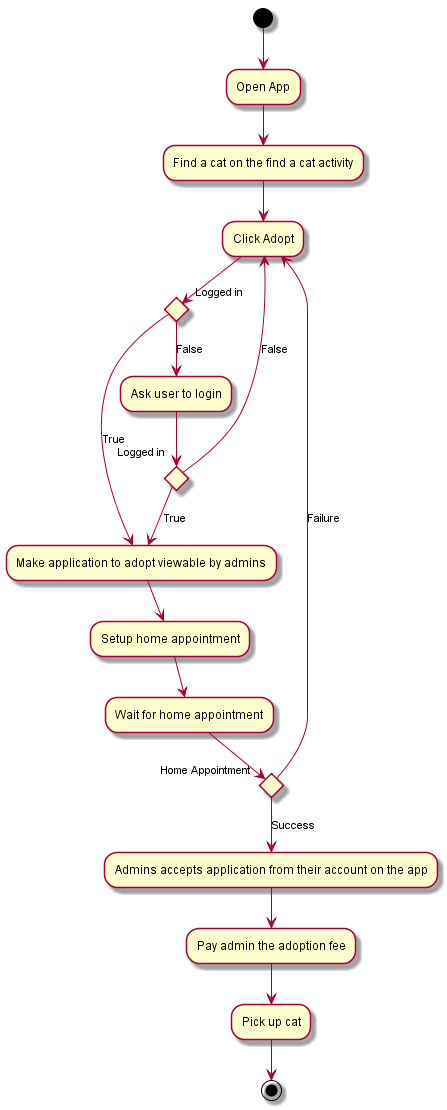
\includegraphics[scale=0.55]{Images/AdoptACat.png}
    \caption{The adoption UML activity diagram, for adopting a cat through the application}
    \label{fig:adoptionProcess}
\end{figure}
%\addcontentsline{toc}{chapter}{Development Process}
\chapter{Design}

This chapter mainly covers the design and processes by which a prototype was designed and implemented. The chapter goes into detail about the intended structure and implementation of the program and UI structure. A significant part of this project consisted of the UI, and its interactions, so much detailed effort is spent on explaining various design decisions and attempting to explain it all goes together into the programming portion of the project.

Firstly, a discussion about the prototype design (Section \ref{PROTOTYPESECTION}), then changes to that design as implementation occurred (Section \ref{DESIGNCHANGESSECTION}), then the code structure and how different parts of the application fit together (Section \ref{CODESTRUCTUREDESIGN}), and finally rounding it up with the design aspects based around accessibility (Section \ref{ACCESSIBILITYDESIGN}).


\section{User Interface Prototyping} \label {PROTOTYPESECTION}
A significant part of the design process in this project was user interface prototyping, it was the main focus of a sprint and was the most significant driving force behind the design of the entire application, so the time spent was justified. I found the process of prototyping to be incredibly valuable when it came to getting my head around what features would make sense, in the context of a native application, against what would not work in the sense of a Material Design based native Android application.

The prototype was created using a web app called Figma \cite{FIGMA}, and my version can be found at this URL \url{https://bit.ly/2xuAvl6}, from here you can see the entire prototype, as well as access a semi-functional version, not all functionality was implemented due to certain limitations with the prototyping software and time limitations. Still, it gives a good idea of how the application was designed and intended to run before any code was written.

\subsection{Colour Scheme} \label{COLOURSCHEME}
In order to stick to Material Design guidelines, I utilised a tool provided by the Material Design website\cite{MATERIALDESIGNCOLOURS} for determining what secondary and aspect colours should be used, given a set of primary colours, that are common across multiple applications. The idea of this colour tool is to promote the idea of applications on Android having similar colour schemes, and a generalised theme across the entire platform. Early on, I liked a darker orange colour as my primary colour (\#ff6f00), I found it looked good in my prototype, and I stuck to it. The colour tool recommended a lighter primary colour (\#ffa040), and a darker primary colour(\#c43e00) for different parts of the application, such as the application navigation bar at the bottom of the phone, or the background of the system bar at the top of the Android phone. The lighter primary colour is often used for accenting or less important parts of the application. With the colour scheme, the text colour of black (\#000000) is recommended.

More modern Android applications, take advantage of a recent trend in UX design, which is the replaceable theme, with a darker version, for night time or general use, these themes use less power and often are easier on the eyes especially in low light environments. With that in mind, with the help of the aforementioned tool for colour picking\cite{MATERIALDESIGNCOLOURS}, I picked a dark variation colour scheme, primary colour (\#424242), primary light colour (\#6d6d6d), primary dark colour (\#1b1b1b), and text colour (white: \#ffffff). The dark theme mostly consists of different variations of the colour grey. To continue the application's theme across both dark and light themes, different parts of the application won't change, such as the title bar's background colour, or the colour of the \gls{Bottom Navigation Bar}'s icons.

The text colour changes based on the background colour, allow users of all abilities to read it easier, for example, white text on a black background is easier to read than a dark blue text on a black background. The same could be said for black text on a white background such as this report if the text were a light yellow, it would be harder to read on this light background.

\subsection{General App Design}

The app design has a few key features shared across multiple screens; this section discusses these key features.

The \gls{Bottom Navigation Bar} is the Material Design inspired navigation method of choice on Android according to the Material Design guidelines (\cite{MATERIALDESIGNGUIDELINES}), the current choice of only allowing navigation to home, cat finder, and saved cats (See Figure \ref{fig:prototype_home}) allows the main actions that users probably want to fulfil, to be the most available to users the moment they open the app. The \gls{Bottom Navigation Bar} allows a user to easily switch between the main screens using only one hand as it is near the base of the phone, is one of the main benefits of it's intended inclusion.

When on one of the main screens (Home, Cat Finder, and Saved Cats), there is the option to access the navigation draw (Section \ref{PROTOTYPENAVIGATIONDRAW}) using the \gls{Hamburger Icon} in the upper left side, featured throughout other Android application designs. However, due to the nature of the app, there are multiple different methodologies for navigation. In Android, there is the \gls{System Bar} and in-app navigation. Material Design has a guideline for navigation draw and navigation, it aims to replace the navigation draw button with an \gls{Up Button}, whenever you are not on any of the main screens, this allows a user to navigate back up the navigation hierarchy in the application quickly, the replacement is done fluidly with an animation. 

If a user navigates to a \gls{Card} from the main screens or a secondary screen, it navigates to either the Adoption Information screen or the Cat Information screen, which allows navigation back using an X button to close the current "pop-up".

It is possible to access the settings from the majority of the app (by clicking the cog icon in the top right of most of the screens in the app). The design is aimed at allowing users to get to the settings as fast as possible from wherever in the app. Quick access to settings is good because of the need to change key settings that may be added in the future for accessibility features or notifications, or if a user just doesn't want to lose their place in the app.

Material design provides a set of icons, the idea of having a single set of defined icons that are supported across multiple devices, applications, and interfaces aim to increase usability, and ease of learning for these devices, applications, and interfaces. The icons are the same across different devices and applications, for example, a settings icon is a cog, or a save icon is the floppy disk. Not only are these icons provided freely under an open license, but they are heavily integrated into the Android Studio integrated development environment.

\subsection{Home Screen}

\begin{figure} [htbp!]
    \centering
    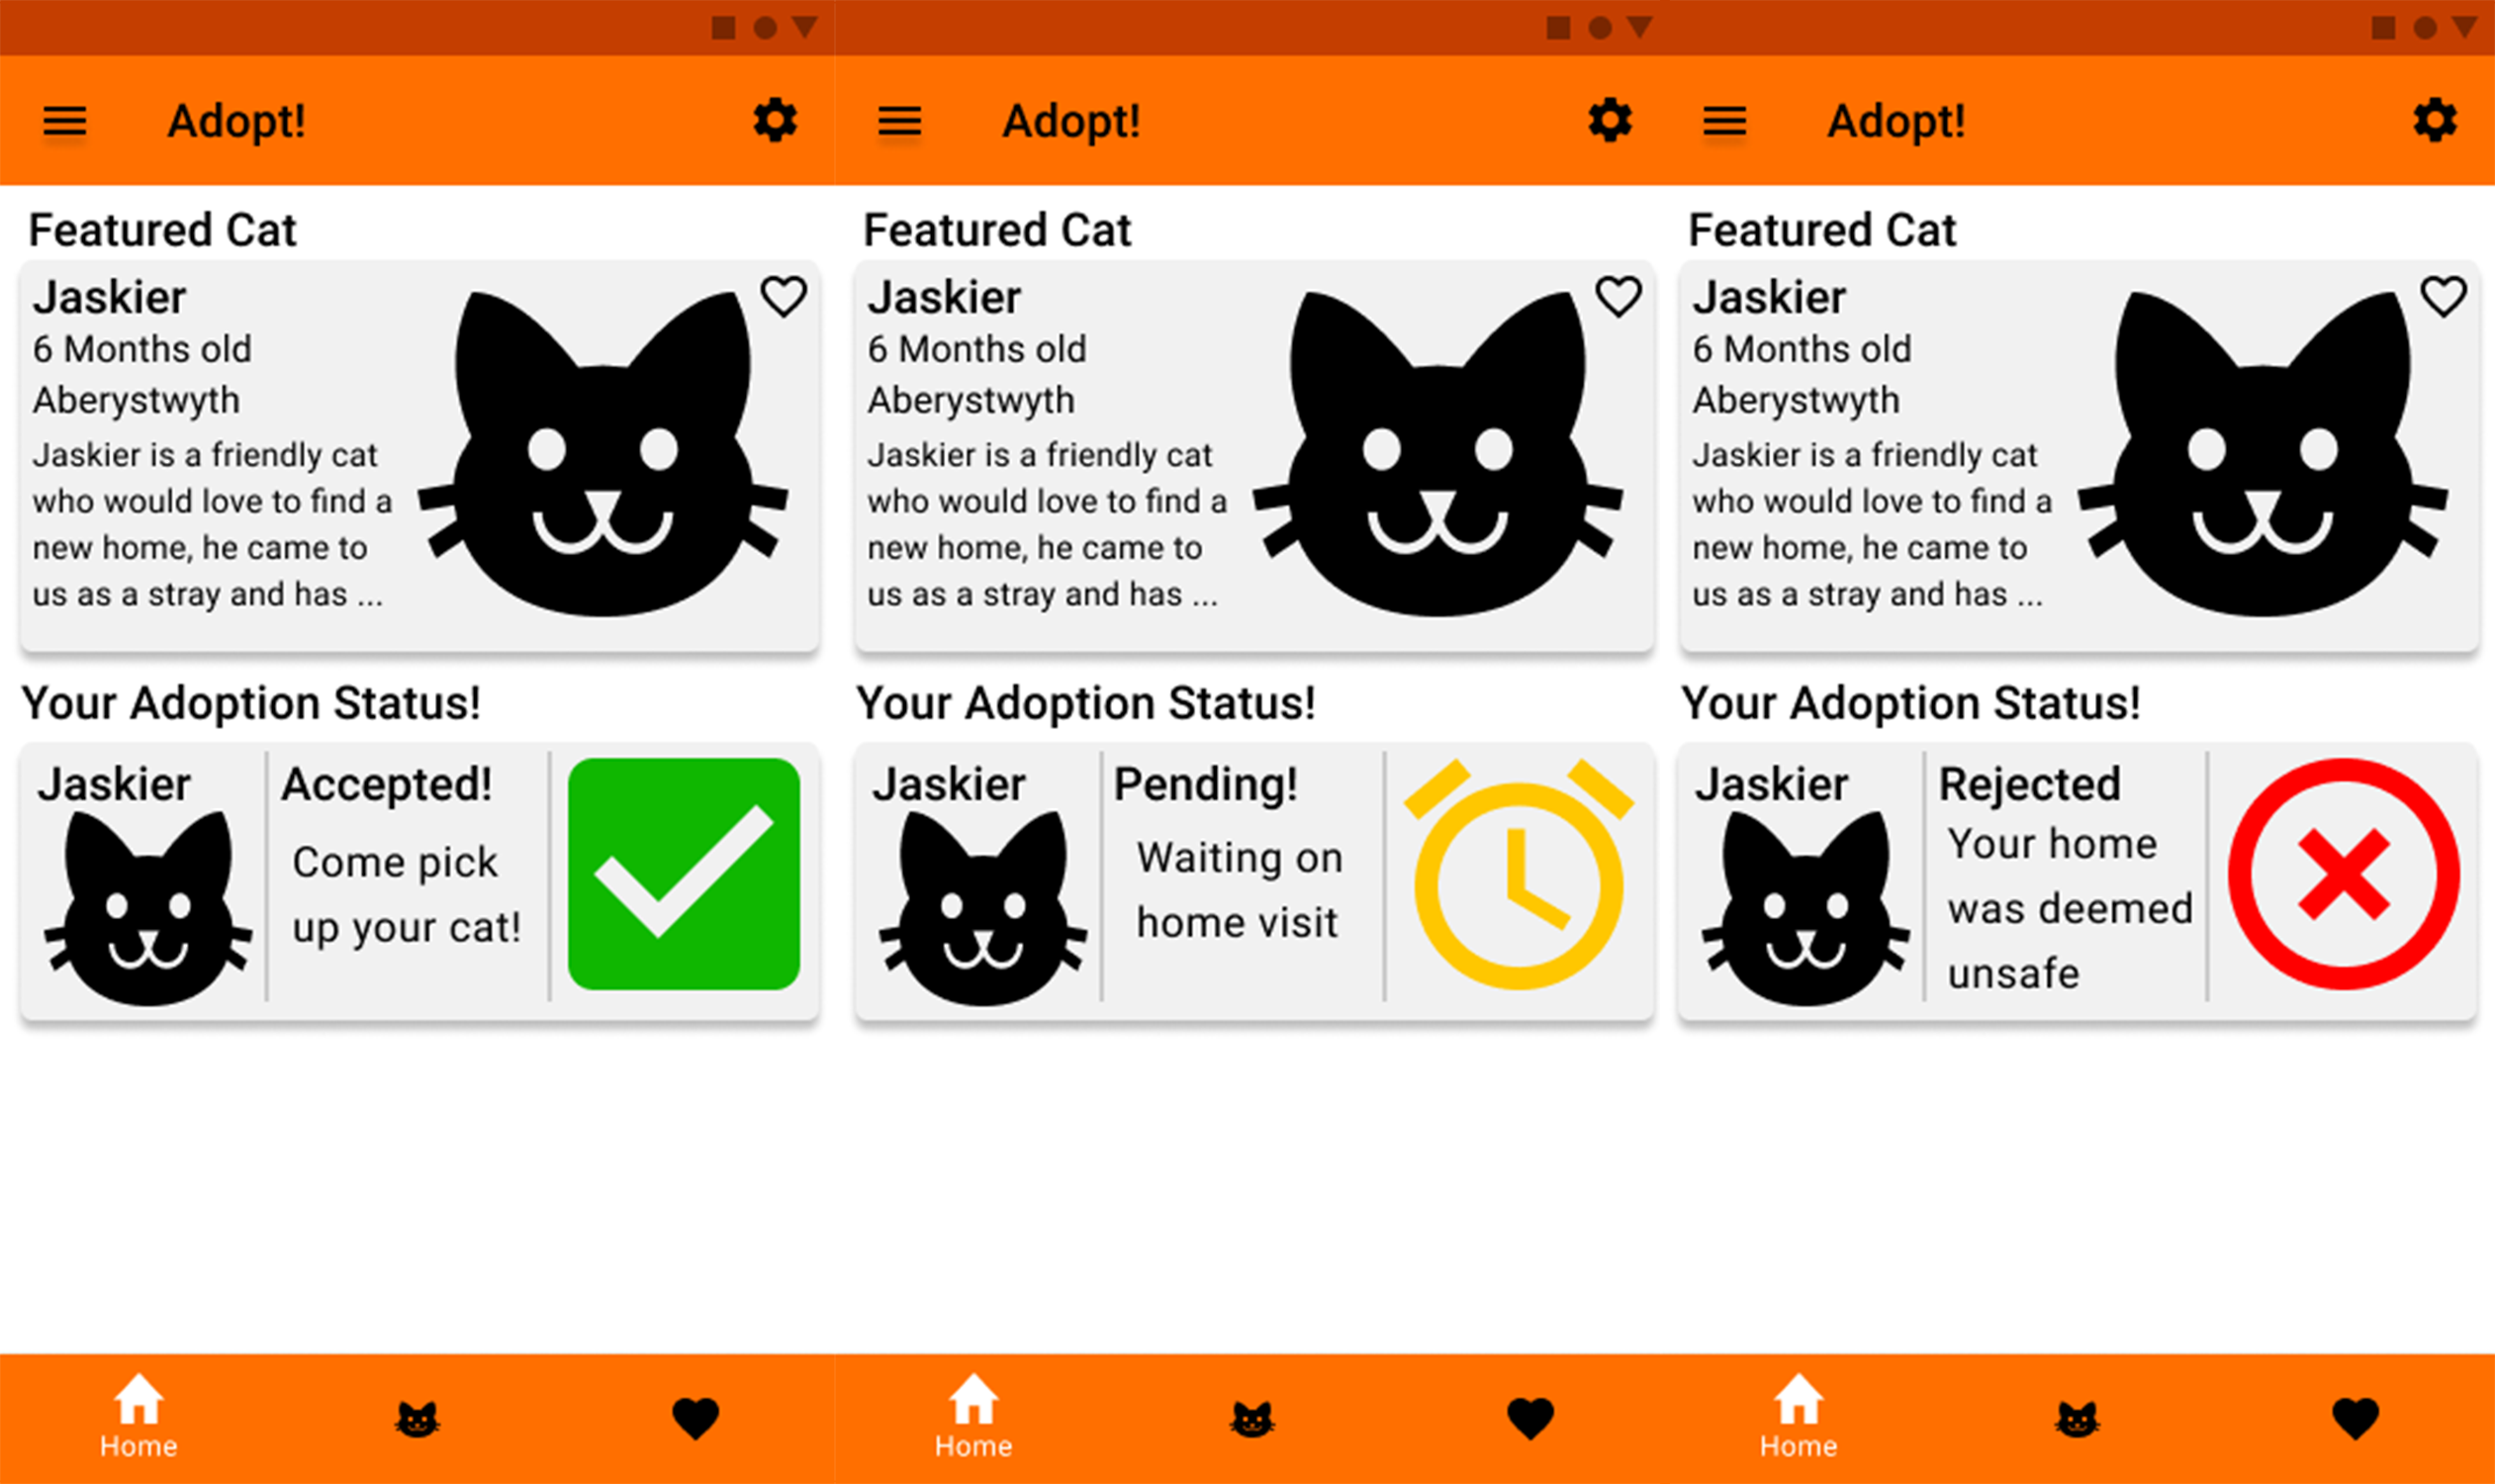
\includegraphics[height=7cm]{Images/PrototypeHomeScreen.png}
    \caption{3 variations of the prototyped home screen}
    \label{fig:prototype_home}
\end{figure}

Figure \ref{fig:prototype_home}, shows the prototype of my home page; it aims to have a randomly picked cat from the back end database showing using a Saved Cat Card (\ref{PROTOTYPESAVEDCATCARD}). On the home page, if logged in, it displays the statuses of your current adoption requests, figure \ref{fig:prototype_home} shows the adoption status cards (\ref{PROTOTYPEADOPTIONSTATUSCARD}) in it's 3 potential states, as there are multiple outcomes from a request if the user is not logged in, then text displays telling them there are not logged in and to login, to use that feature. My thought process with this layout was based around the idea of what people want to see the most, people want to see a cat to adopt, and most importantly users want to see their adoption status as soon as possible.

\subsection{Cat Finder Screen}

\begin{figure} [htbp!]
    \centering
    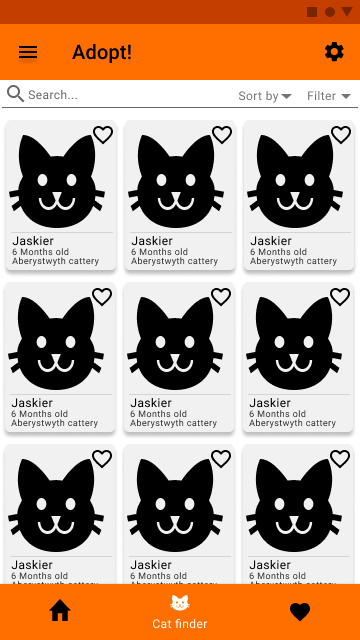
\includegraphics[height=7cm]{Images/PrototypeCatFinder.png}
    \caption{Prototype cat finder screen}
    \label{fig:prototype_cat_finder}
\end{figure}

The Cat finder screen is intended for users to find a cat to adopt, to allow for this it requires cats to be displayed similar to how Amazon or eBay lists products, as they are great inspirations for displaying options. In line with that, I included Search, Sort by and Filter functionality found in many e-commerce implementations, both on mobile and not, it has become a staple and expected feature of many places offering both products for sale and websites advertising cats for adoption, including Cats Protection \cite{CATSPROTECTION}. The prototype intends for up to 3 cats to be shown in a row and the ability to effectively scroll infinitely down to the bottom of all of the cats stored in our systems.

The cats are displayed using a \gls{Card} (Section \ref{PROTOTYPECATCARD}) designed precisely for this purpose. The \gls{Card} shows a scaled-down image of the cat, its name, its age in a transparent manner, and its location of residence. The \gls{Card} allows a user to click on it and have a look at further information, in the Cat Information screen (Section \ref{PROTOTYPECATINFORMATIONSCREEN}). 

\subsection{Saved Cats Screen}

\begin{figure} [htbp!]
    \centering
    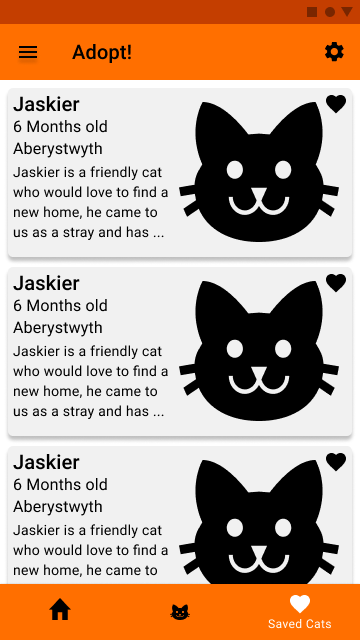
\includegraphics[height=7cm]{Images/PrototypeSavedCats.png}
    \caption{Prototype saved cats screen}
    \label{fig:prototype_saved_cats}
\end{figure}

The saved cats screen is where a user can see (once logged in) all of the cats they have favourited/saved using the heart icon found throughout the application closely associated with a cat. It displays all these cats in its \gls{Card} variation called Saved Cat Card (Section \ref{PROTOTYPESAVEDCATCARD}). Each \gls{Card} has its layer and display every single cat that has been favourited in this format even if that includes every single cat in the system.

\subsection{Saved Cat Card} \label{PROTOTYPESAVEDCATCARD}

\begin{figure} [htbp!]
    \centering
    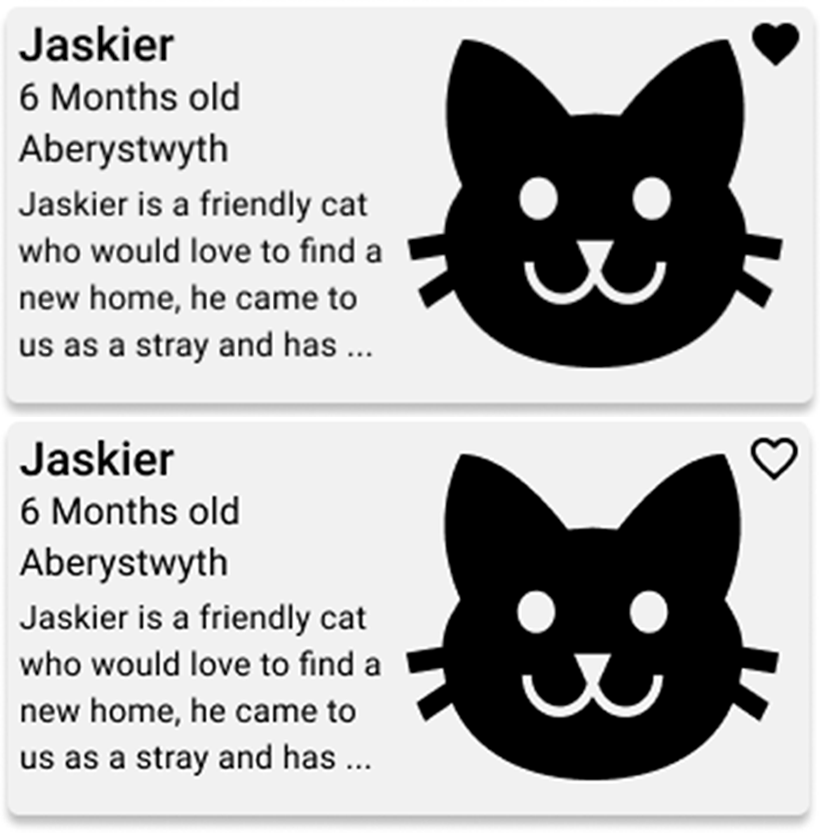
\includegraphics[height=5cm]{Images/PrototypeSavedCatCard.png}
    \caption{Prototype saved cat card}
    \label{fig:prototype_saved_cat_card}
\end{figure}

The Saved cat card is used in multiple parts of the app and is a versatile method for displaying information, it shows the start of the description for the cat, alongside its name, age, and location much like other cat cards. This \gls{Card} also shows a larger version of the cat's scaled-down image, and a favourite button represented by either an empty or full heart, depending on whether the cat has been saved or not, if saved then it is filled, if not saved then it is not filled. This \gls{Card} functions largely the same as the Cat Card (Section \ref{PROTOTYPECATCARD}).

The reason there is a more detailed card for cats of more interest is that they are of a higher interest to potential adopters than the other cats listed in the application. The other cats are not saved or featured for any specific reason, due to the volume of cats more detail can't be shown, but with these more special interest cats, they can have the attention that it requires given with this more detailed \gls{Card}.

\subsection{Adoption Status Card} \label{PROTOTYPEADOPTIONSTATUSCARD}

\begin{figure} [htbp!]
    \centering
    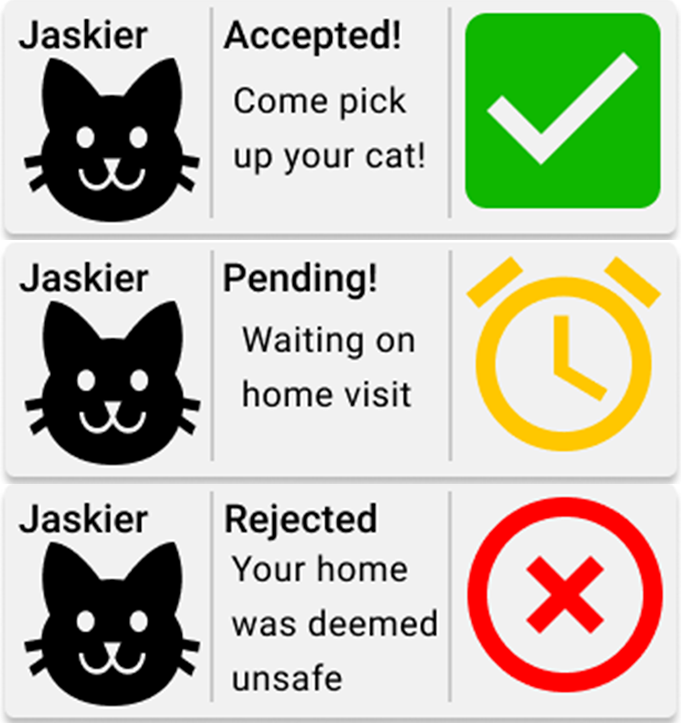
\includegraphics[height=6cm]{Images/PrototypeAdoptionCards.png}
    \caption{Prototype adoption status card}
    \label{fig:prototype_adoption_status_card}
\end{figure}

The adoption status \gls{Card} has 2 purposes, to display the current state of an adoption request, this has 3 major states, accepted, pending/being processed, and rejected. Alongside the major states, there are more nuanced details added to it, at present they are pretty basic, but if a person's application is rejected, then it says why, if a user's application is pending it says why. The \gls{Card} includes the name and picture of the cat, so a user knows which cat this adoption application is related to, as a user may have more than one adoption request, rejected or otherwise.

If you click on this \gls{Card} much like any other \gls{Card} it will expand to show more information, the information it shows is relevant to the adoption status and is discussed in section \ref{PROTOTYPEADOPTIONSTATUSINFOMATION}.

\subsection{Cat Card}\label{PROTOTYPECATCARD}

\begin{figure} [htbp!]
    \centering
    
\includegraphics[height=3cm]{Images/PrototypeCatCard.png}
    \caption{Prototype cat card}
    \label{fig:prototype_cat_card}
\end{figure}

The base-level Cat \gls{Card} is the primary way a user will first see their future cats; it is the primary method from which a user is expected to interact with a cat. It's a small compact area to display essential information related to the cat. The most key information was decided to be, what the cat looked like, the name, its age, and location in that order. The order of importance for information is displayed in this Cat \gls{Card}, as top-down. The cat card does allow for quick saving/favouriting as long as a user is logged in, much like the Saved Cat \gls{Card}, by tapping the button in the top right shaped like a heart, if not filled the cat is not saved, if filled then the cat has already been saved by that user, and can be used to unsaved the cat.

If the Cat \gls{Card} is clicked/tapped then the user will be navigated to the respective cat's Cat Information screen. (Section \ref{PROTOTYPECATINFORMATIONSCREEN})
\subsection{Adoption Status Screen} \label{PROTOTYPEADOPTIONSTATUSINFOMATION}

\begin{figure} [htbp!]
    \centering
    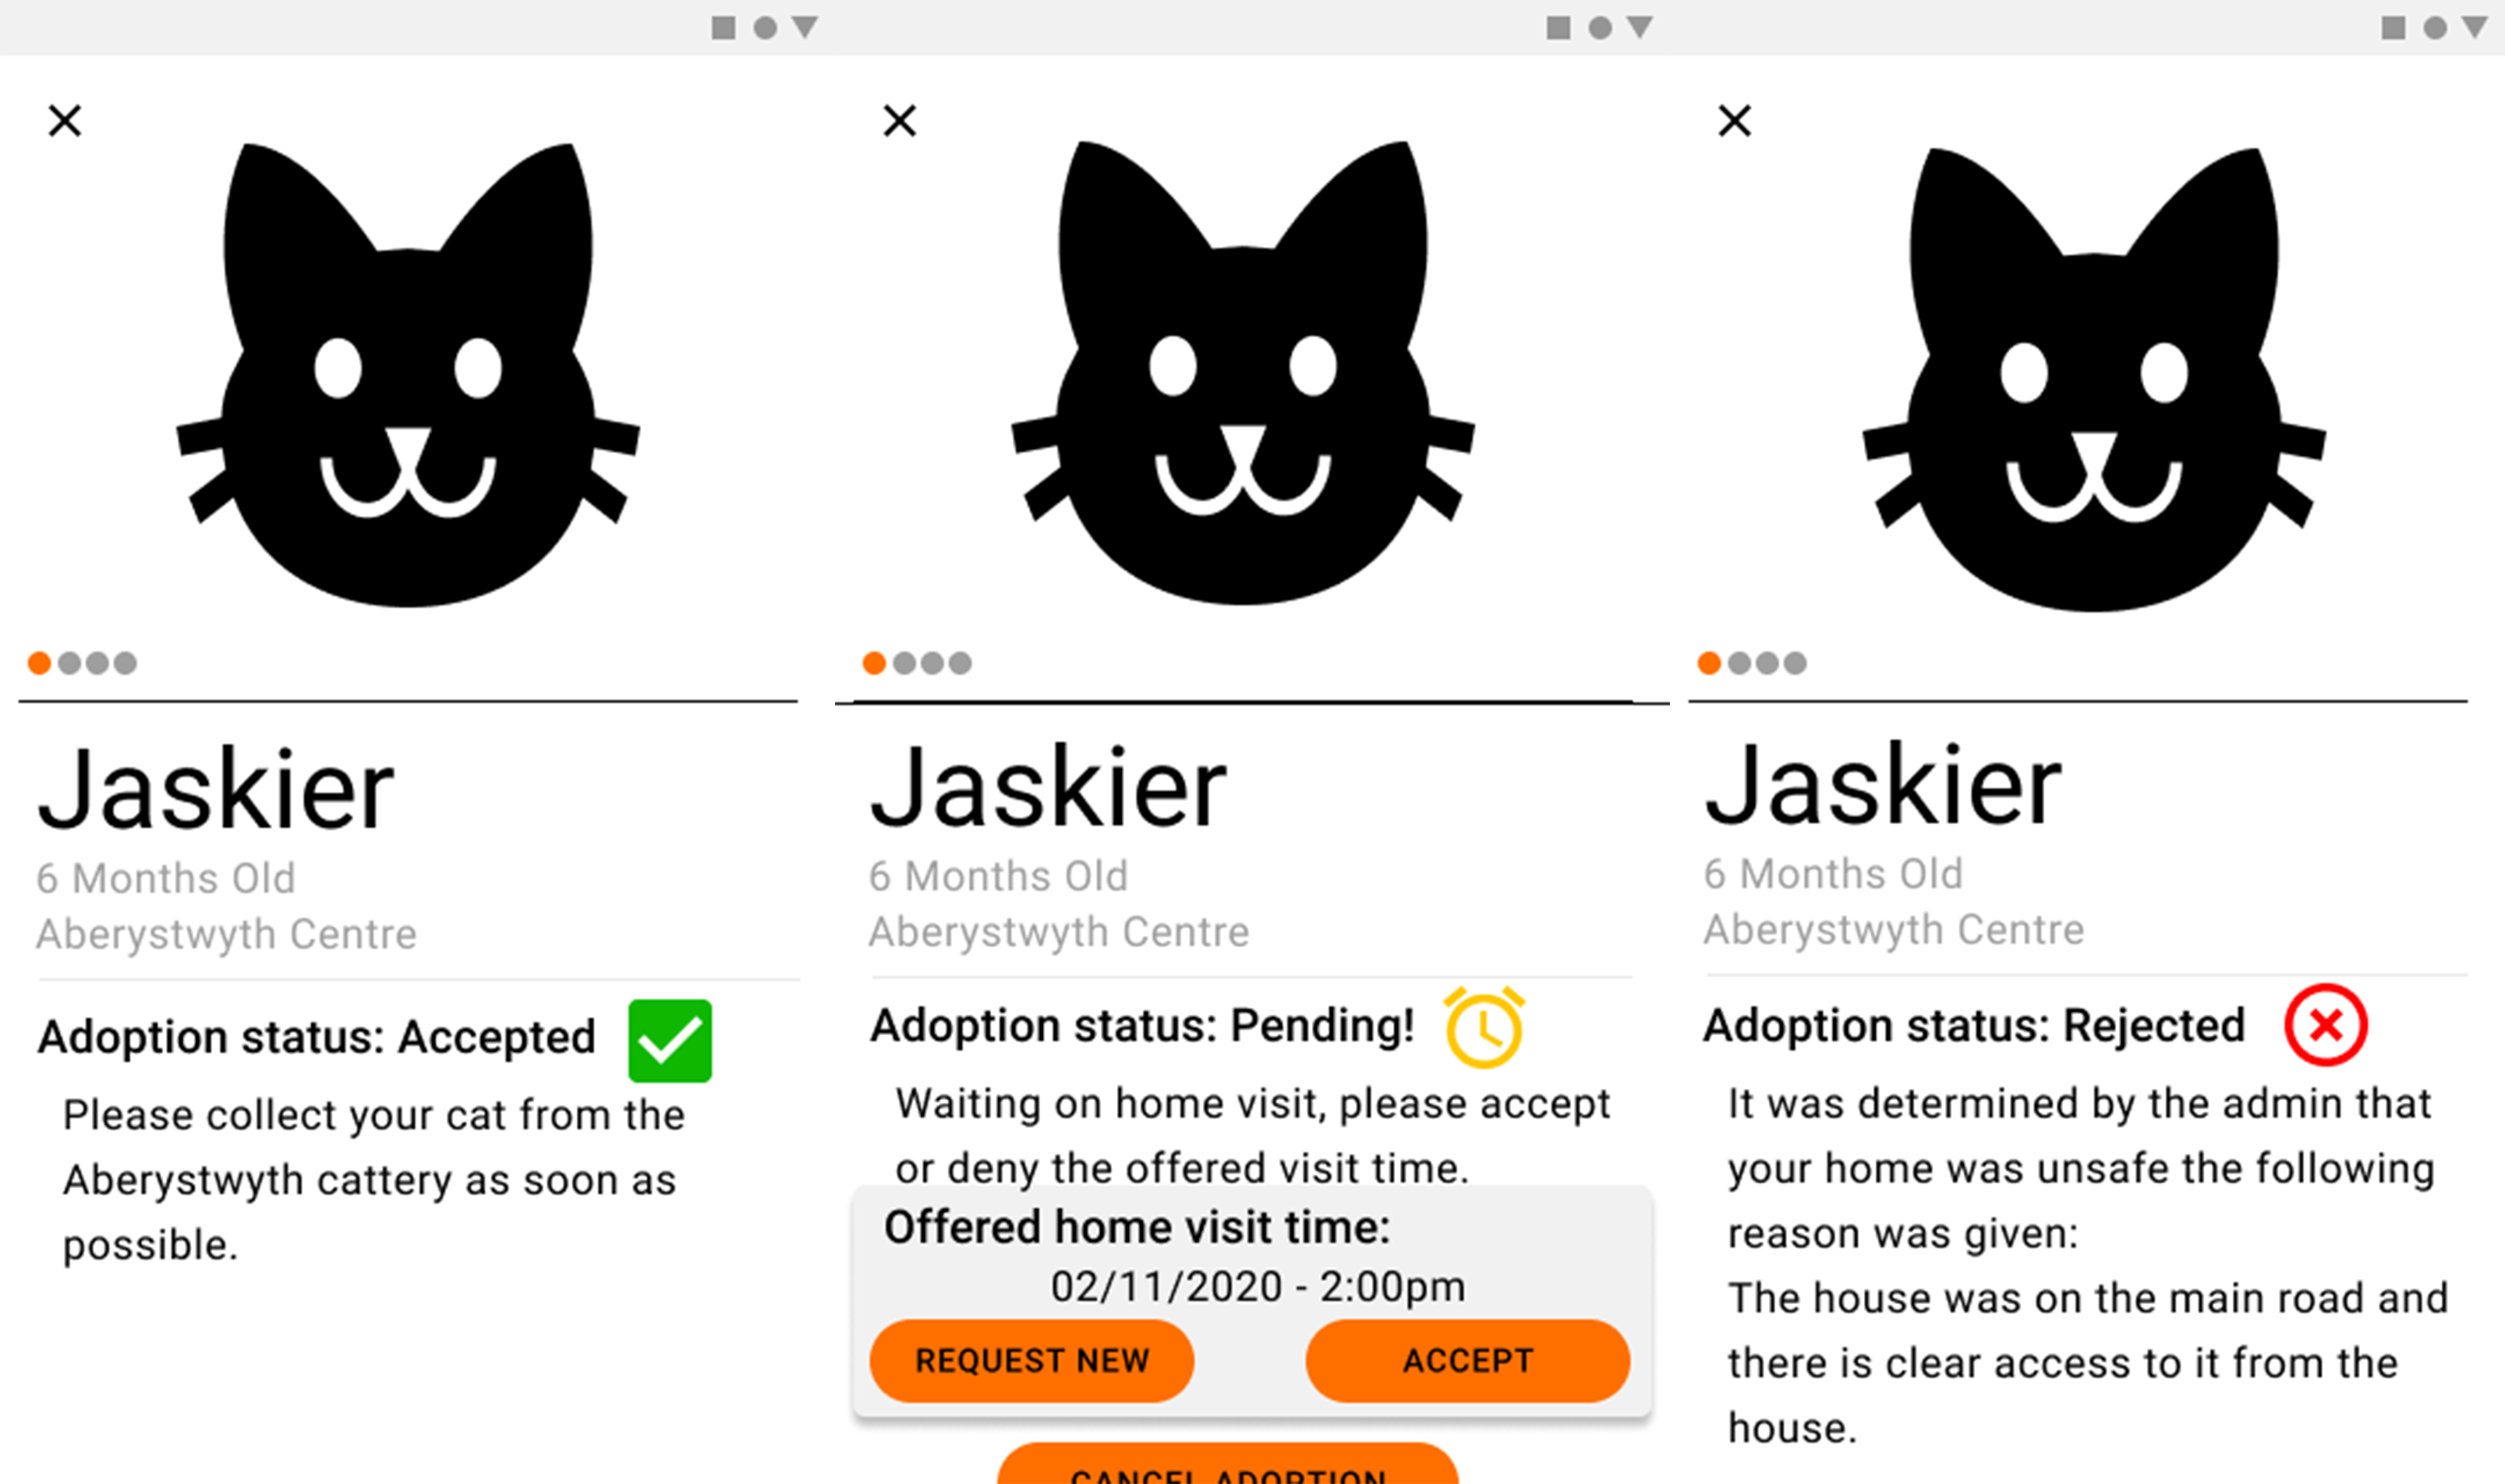
\includegraphics[height=7cm]{Images/PrototypeAdoptionStatusInfomation.png}
    \caption{Prototype more adoption information screen}
    \label{fig:prototype_adoption_status_infomation}
\end{figure}

The design for this screen is mostly the same as the prototype cat information screen (Section \ref{PROTOTYPECATINFORMATIONSCREEN}). A cross replaces the up/navigation draw button as now, and you may want to close the screen and return, it will not strictly be an up navigation as it is technically a pop-up. The cat, name, age and location are shown to reinforce to a user that they are looking at the correct cat's adoption form.

The adoption status screen portrayed in this prototype allows for the acceptance of appointments or requesting of new appointments, further details as to why your application may have been accepted, rejected, or still pending. Finally, it allows for a user to cancel their adoption request if it is still pending. Rejected ones are not removable, and neither are accepted ones, not that a user necessarily wants to do that if so it is possible outside of the application by an administrator.

\subsection{Navigation Draw} \label{PROTOTYPENAVIGATIONDRAW}

\begin{figure} [htbp!]
    \centering
    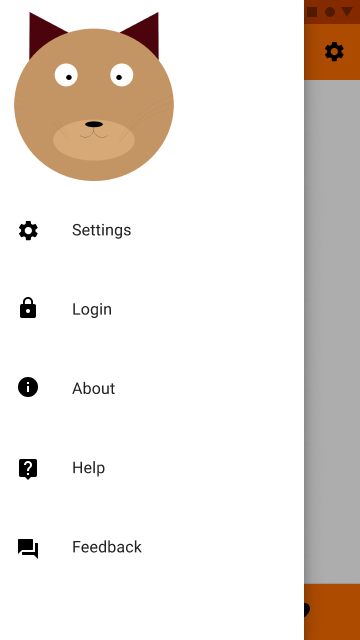
\includegraphics[height=7cm]{Images/PrototypeNavDraw.png}
    \caption{Prototype navigation draw}
    \label{fig:prototype_nav_draw}
\end{figure}

This is a prototype bare-bones navigation draw (Figure \ref{fig:prototype_nav_draw}) to allow navigation to more rarely visited parts of the app, here you can access your login/my account, about, help, and feedback screens in the application. These are not used regularly, but they do allow users access to more information from the app, the navigation draw was added in conjunction with the \gls{Bottom Navigation Bar} to allow the user to navigate to these but more hidden than the Bottom Navigation Bar.

The idea is to have the navigation draw, include a logo and below that the actual navigation locations.

\subsection{Login Screen}

\begin{figure} [htbp!]
    \centering
    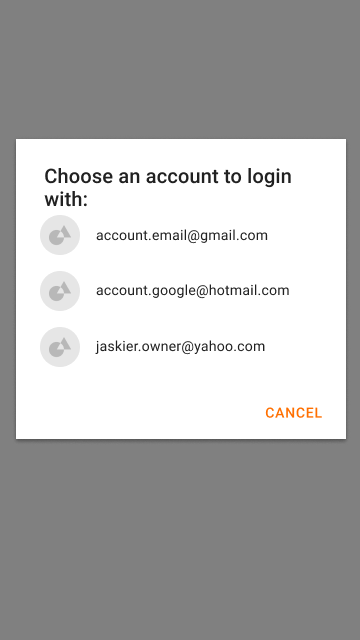
\includegraphics[height=7cm]{Images/PrototypeLoginScreen.png}
    \caption{Prototype login screen}
    \label{fig:prototype_login_screen}
\end{figure}

The screen here is a place holder (Figure \ref{fig:prototype_login_screen}). I expect this to change with the implementation of technology, at the time of designing the specific technology has not been chosen. The intention is to allow a user to login, using at least google if not different accounts.

\subsection{My Account} \label{PROTOTYPEMYACCOUNTPAGE}

\begin{figure} [htbp!]
    \centering
    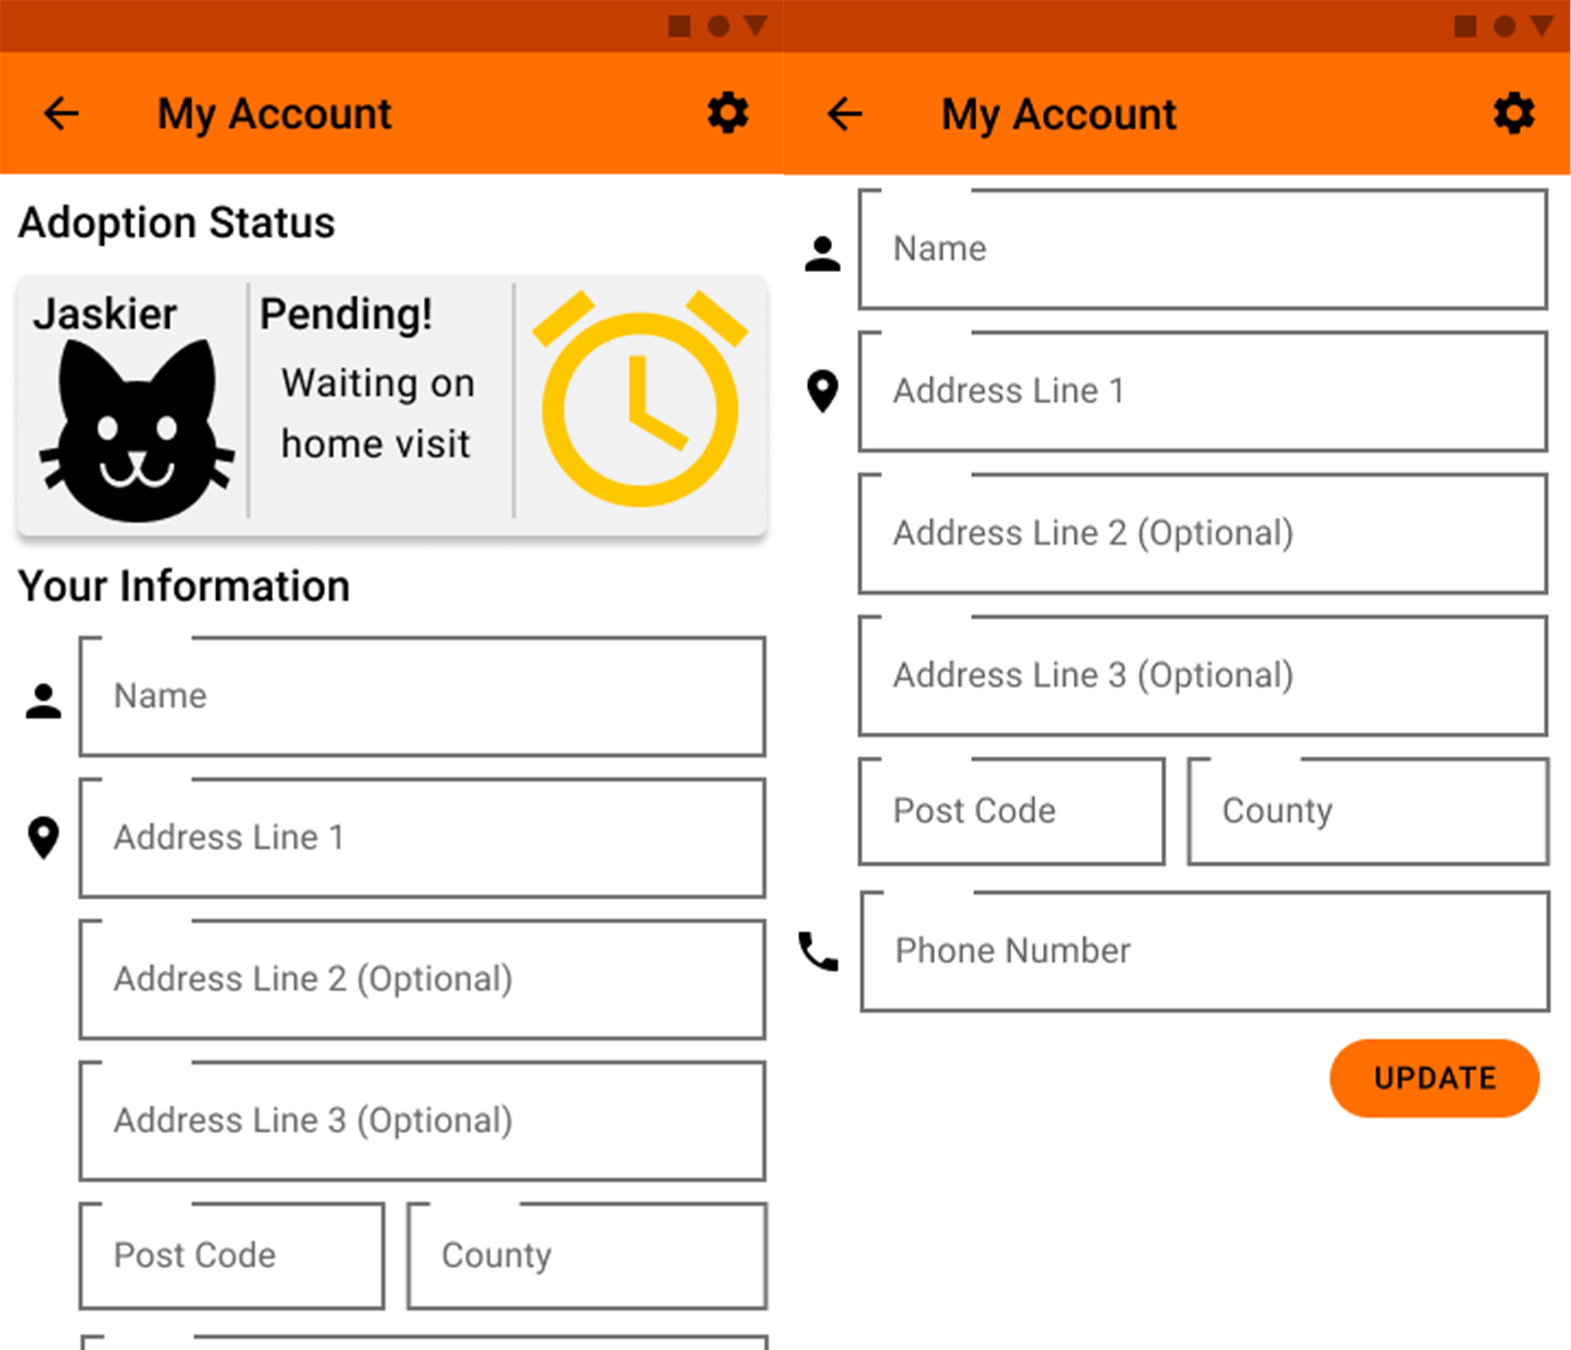
\includegraphics[height=7cm]{Images/PrototypeMyAccount.png}
    \caption{Prototype account screen}
    \label{fig:prototype_account_screen}
\end{figure}

The account screen shows current adoption statuses using the Adoption Status Cards (Section \ref{PROTOTYPEADOPTIONSTATUSCARD}), and all of them are shown in the account, even if that is not clear from the prototype. 

From this screen the users can also update their current details so an administrator can call or arrive on time to inspect the premises, these details can be updated by filling in the text fields and clicking update, it is also auto-filled by data from the database should it already be there to avoid overwriting the same data.

Ideally, there would be a place to logout here; this is done during implementation and is not shown in the prototype as it was an oversight.

\subsection{Settings}

\begin{figure} [htbp!]
    \centering
    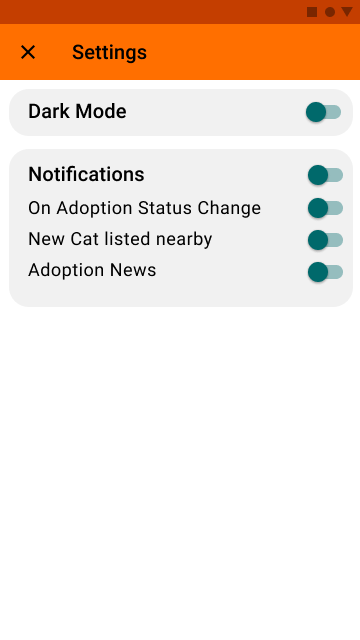
\includegraphics[height=7cm]{Images/PrototypeSettings.png}
    \caption{Prototype settings screen}
    \label{fig:prototype_settings_screen}
\end{figure}

The settings tab here is bare-bones, also it is up for debate whether or not the notifications should be in the application or not, based on the fact that Android 10 requires all of these settings to be in the system settings for this application anyway. Dark Mode is potentially system level as well but is currently only expected to work at the application level. 

Other settings can easily be added or removed based on future expansion, and this is only implemented to a basic level.

\subsection{About}

\begin{figure} [htbp!]
    \centering
    
\includegraphics[height=7cm]{Images/PrototypeAbout.png}
    \caption{Prototype about screen}
    \label{fig:prototype_about_screen}
\end{figure}

The About section is a section aimed at giving the appropriate notice and thanks inside of the software for the use of software, font, and icon licenses and explicitly thanks the creators of the fonts and icons made by others in accordance with their licensing. The about page also gives the location of the distributed open-source code of the project, alongside appropriate mention of its open-source license under Apache 2.0 (\cite{APACHE2LICENSE}), this is a static page and does not change, unless via version update.

\subsection{Help}

\begin{figure} [htbp!]
    \centering
    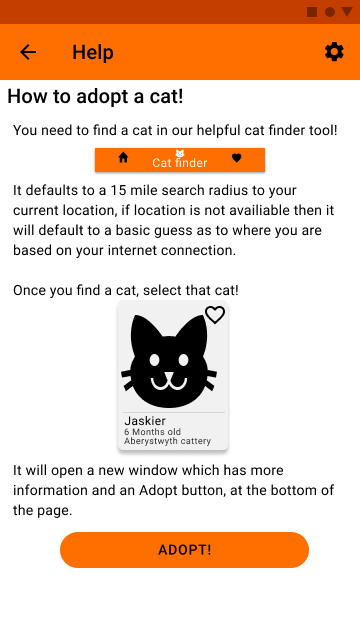
\includegraphics[height=7cm]{Images/PrototypeHelp.png}
    \caption{Prototype help screen}
    \label{fig:prototype_help_screen}
\end{figure}

The help page is another static page, and this page is intended to offer guidance to the user on how to adopt a cat and provides a basic guideline using static images and static text that should assist in the adoption of a cat.

\subsection{Feedback}

\begin{figure} [htbp!]
    \centering
    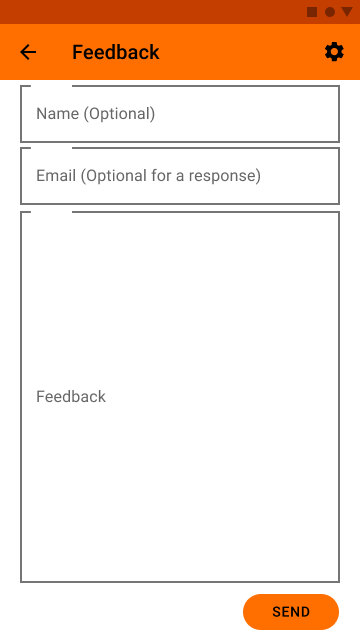
\includegraphics[height=7cm]{Images/PrototypeFeedback.png}
    \caption{Prototype feedback screen}
    \label{fig:prototype_feedback_screen}
\end{figure}

Feedback allows a logged-in user to give feedback on the application straight to the developers, and feedback can help with the applications development, a developer's awareness of bugs etc. Requiring a user to login before providing feedback is a spam avoidance mechanism, where feedback is tied to a user's identifier, meaning if they are spamming feedback from them can be easily removed and blocked from further spam.

\subsection{Cat Information Screen} \label{PROTOTYPECATINFORMATIONSCREEN}

\begin{figure} [htbp!]
    \centering
    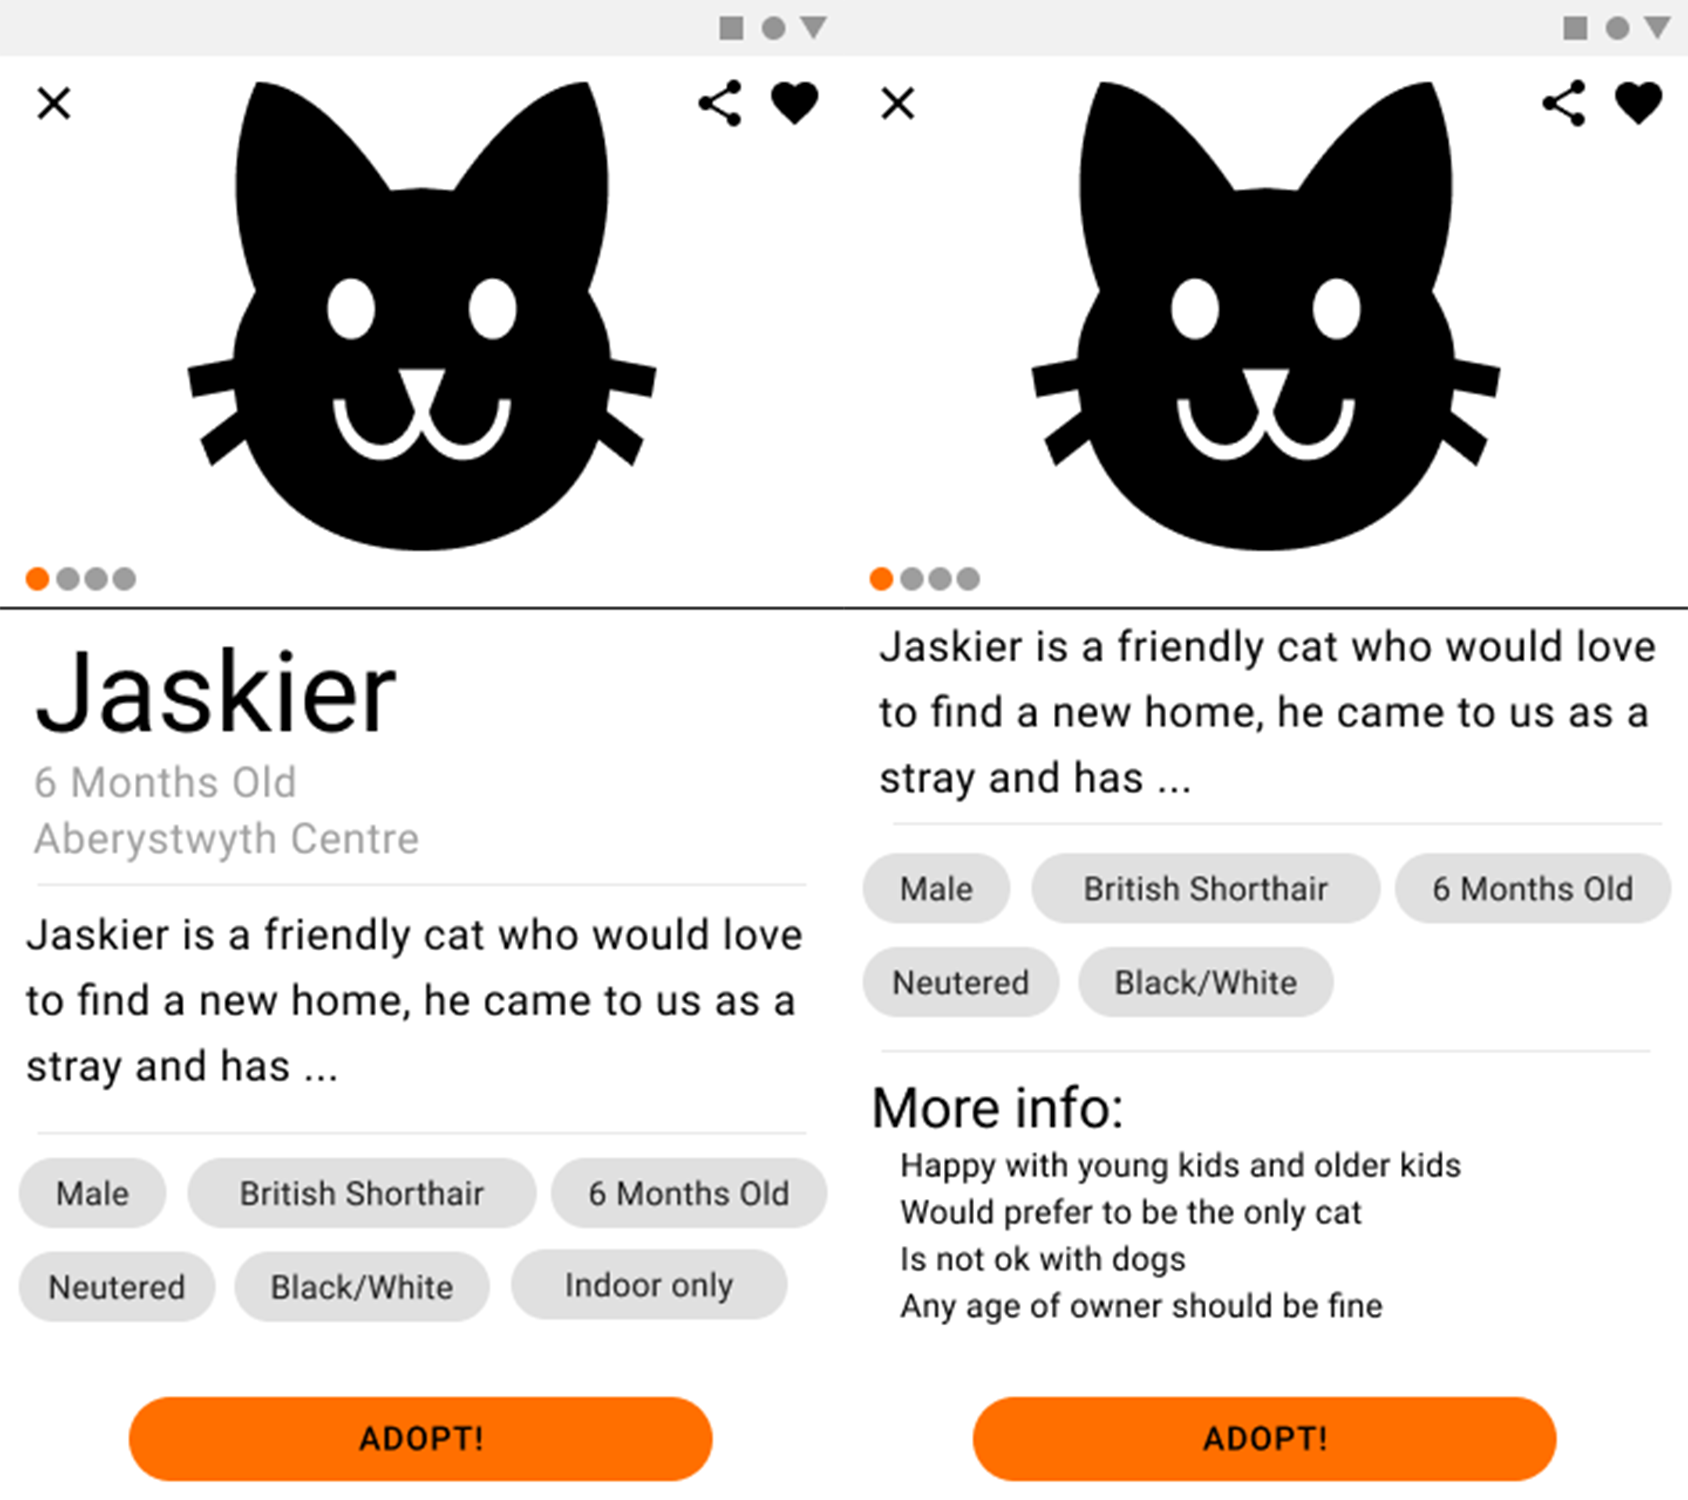
\includegraphics[height=7cm]{Images/PrototypeCatInfo.png}
    \caption{Prototype cat information screen}
    \label{fig:prototype_cat_info_screen}
\end{figure}

The cat information screen is key to showing more details to a user about a specific cat, it was inspired by Material Design Guidelines \cite{MATERIALDESIGNGUIDELINES}, for its theme and layout. It informs a user if the cat likes other cats, dogs, children of multiple different age ranges, whether it is disabled, indoors only or outside, neutered or not, breed, sex, and colour. The screen allows you to adopt the cat, as well as save or share the cat with your friends. The screen also has a description that is written by a volunteer or Foster carer that cares for the cat, and this adds some personality and more adopt-ability to the cat. 

This prototype includes multiple pictures of this one cat, and this may be infeasible later due to the fact that most freely available cat photos under creative commons or other open licenses are of individual cats and not collections of photos of one cat. The process for adding more than one cat picture should not be laborious, the limiting factor is actual images.

The screen does show the same information from the Cat \gls{Card} but it is more prominent as to follow Material Design guidelines for showing more information after interacting with a Material Design \gls{Card}.

\subsection{Adoption Form}

\begin{figure} [htbp!]
    \centering
    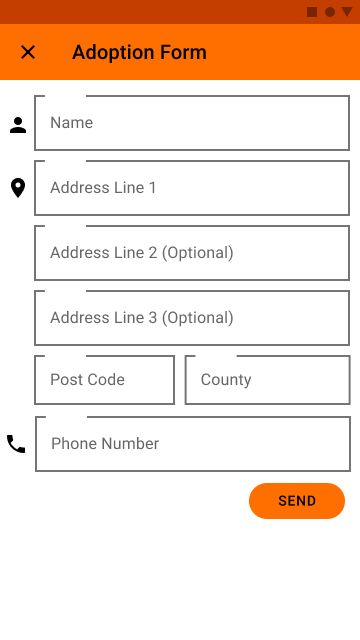
\includegraphics[height=7cm]{Images/PrototypeAdoptForm.png}
    \caption{Prototype adoption form screen}
    \label{fig:prototype_adoption_form_screen}
\end{figure}

The user must update the information in this page before adopting, before getting to this page, a user must be logged in, so the data on this page is synced with the My Account page (Section \ref{PROTOTYPEMYACCOUNTPAGE}). The reason this page must be updated is that an administrator will either ask for an appointment from the most local cattery/centre or a user should be contacted via phone, email, or mail to confirm details of the application etc. This information will be crucial to the adoption process.

\section{User interface design changes during implementation} \label{DESIGNCHANGESSECTION}
Some parts of the application have changed since the initial prototyping, and these features are detailed below in the relevant subsections. Different parts of the application prototype did not either feel right or align well with Material Design, as the project went on I reviewed and updated the designs as I implemented, reviewing the Material Design guidelines with each feature implementation \cite{MATERIALDESIGNGUIDELINES}. Some changes are not discussed here because of the nature of implementing design as an actual application and how things perform on certain devices.

\subsection{Addition of a Dark Mode Scheme}

\begin{figure} [htbp!]
    \centering
    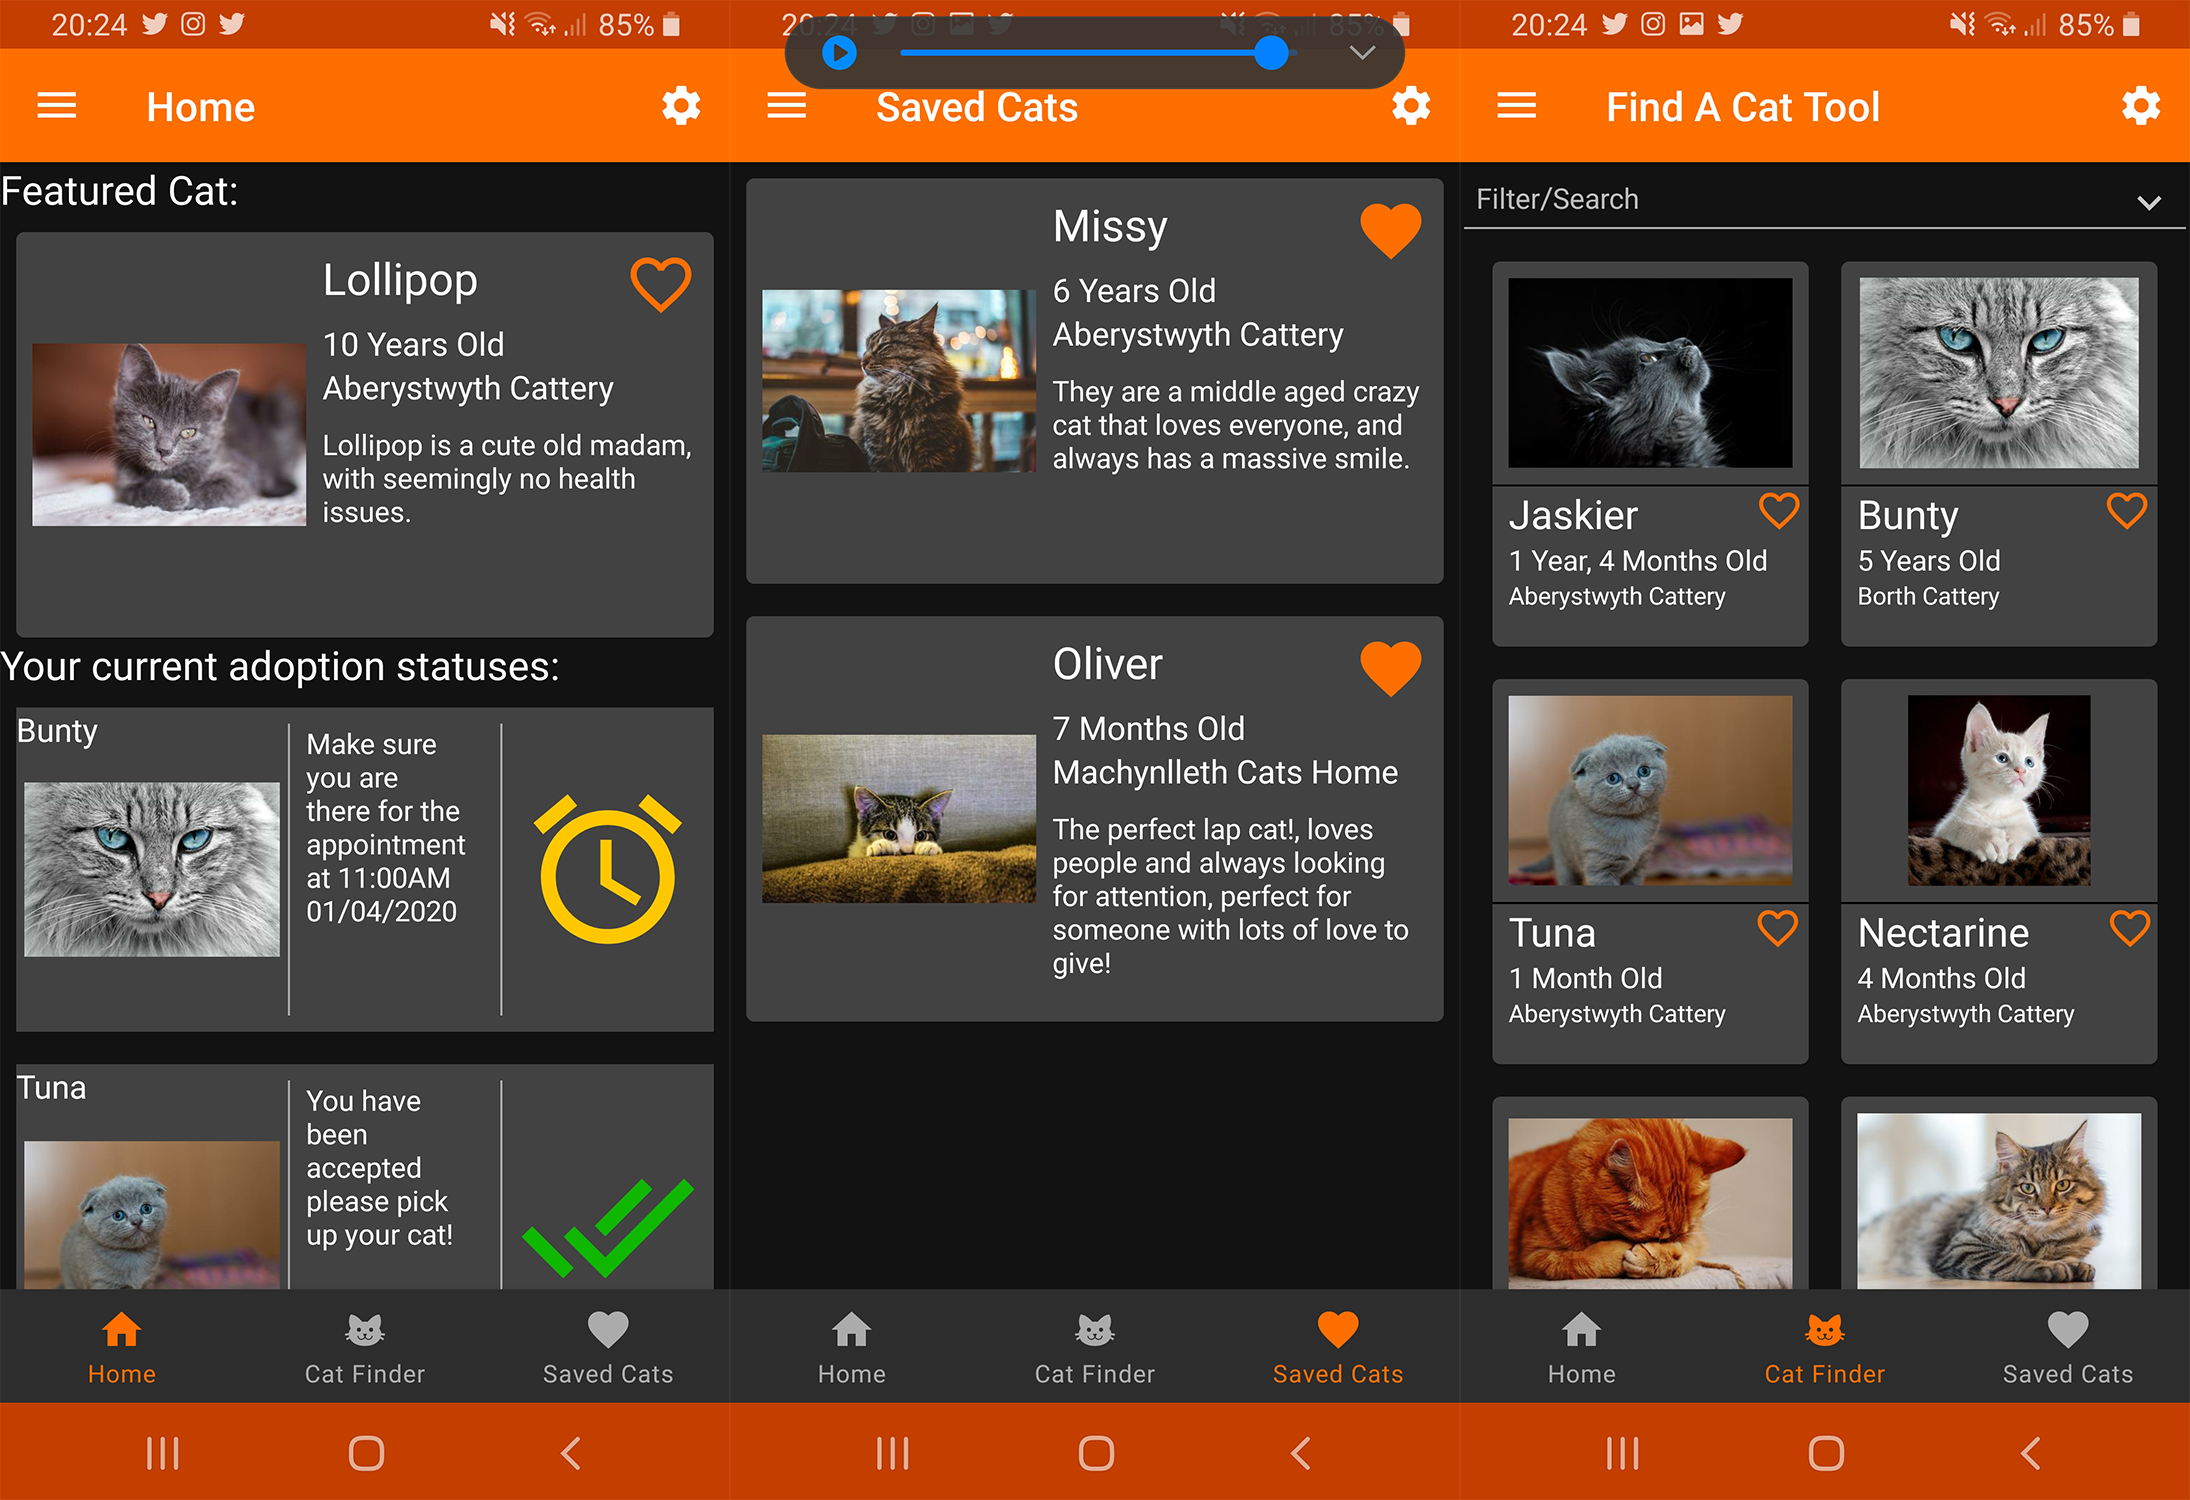
\includegraphics[height=7cm]{Images/DarkMode.png}
    \caption{Example of dark mode changes}
    \label{fig:dark_mode}
\end{figure}

During implementation it became apparent that Android developers are moving to dark mode being integrated into their application, this was addressed early in the prototype, and I believe that a darker variation of an application is often easier to use. Dark mode has been implemented using the colour scheme discussed earlier in the report in Section \ref{COLOURSCHEME}. The reason this differs from the prototype is that this was not explicitly designed in the prototype.

Dark mode is discussed in the Material Design guidelines as a feature that reduces battery drain while maintaining the same level of colour contrast. Dark themes also assist with eye strain, lowering required brightness, and allowing a user to use your application in dark areas.

\subsection{Global Navigation Structure}

\begin{figure} [htbp!]
    \centering
    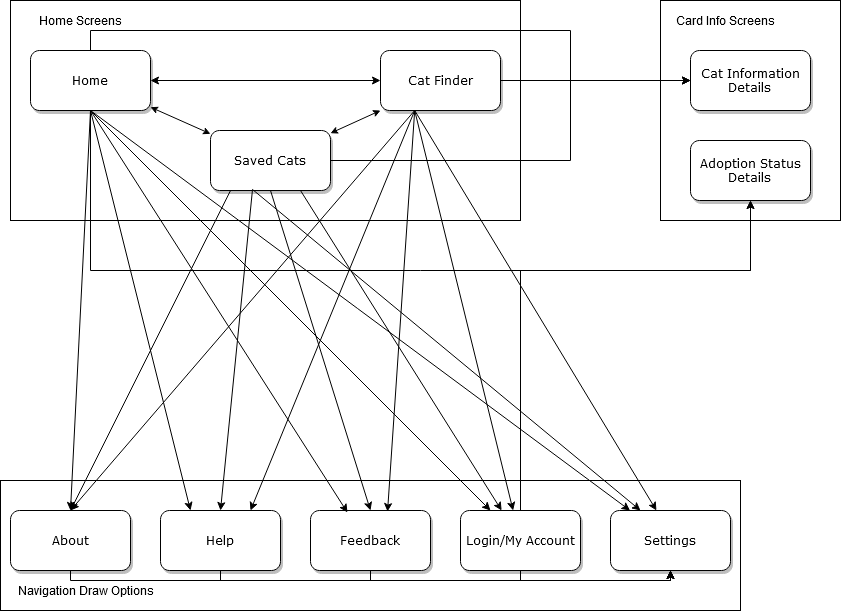
\includegraphics[width=\textwidth]{Images/Navigation Web.png}
    \caption{Theoretical navigation structure}
    \label{fig:global_structure}
\end{figure}

The global navigation structure is centred around the HomeFragment, and for usage, with the NavigationUI all screens are technically navigated to via the HomeFragment screen. However, the actual structure is designed slightly differently, for example, each \gls{Card} navigates to their respective extra information screen, not the HomeFragment, as most cards are not on the HomeFragment screen but, Cat Finder, Saved Cats, or My Account screens. You can see the theoretical navigation web at figure \ref{fig:global_structure}.

\subsection{Bottom Navigation Bar Colour Change}

\begin{figure} [htbp!]
    \centering
    
\includegraphics[height=2cm]{Images/BottomNavigationBar.png}
    \caption{Implementation of Bottom Navigation Bar}
    \label{fig:bottom_navigation_bar}
\end{figure}

In an attempt to stick strictly to Material Design guidelines with colour, the original \gls{Bottom Navigation Bar} from the earlier prototype versions that can be seen in multiple figures throughout this chapter, we have to change the design in order to portray a light and dark theme accurately. The bottom navigation bar was changed to a white background, with the primary colour as the way of determining which navigation location has been selected. All other icons from the one that is selected are greyed out. This is visible in Figure \ref{fig:bottom_navigation_bar}.

\subsection{Cat Finder Layout and Cat Card}

\begin{figure} [htbp!]
    \centering
    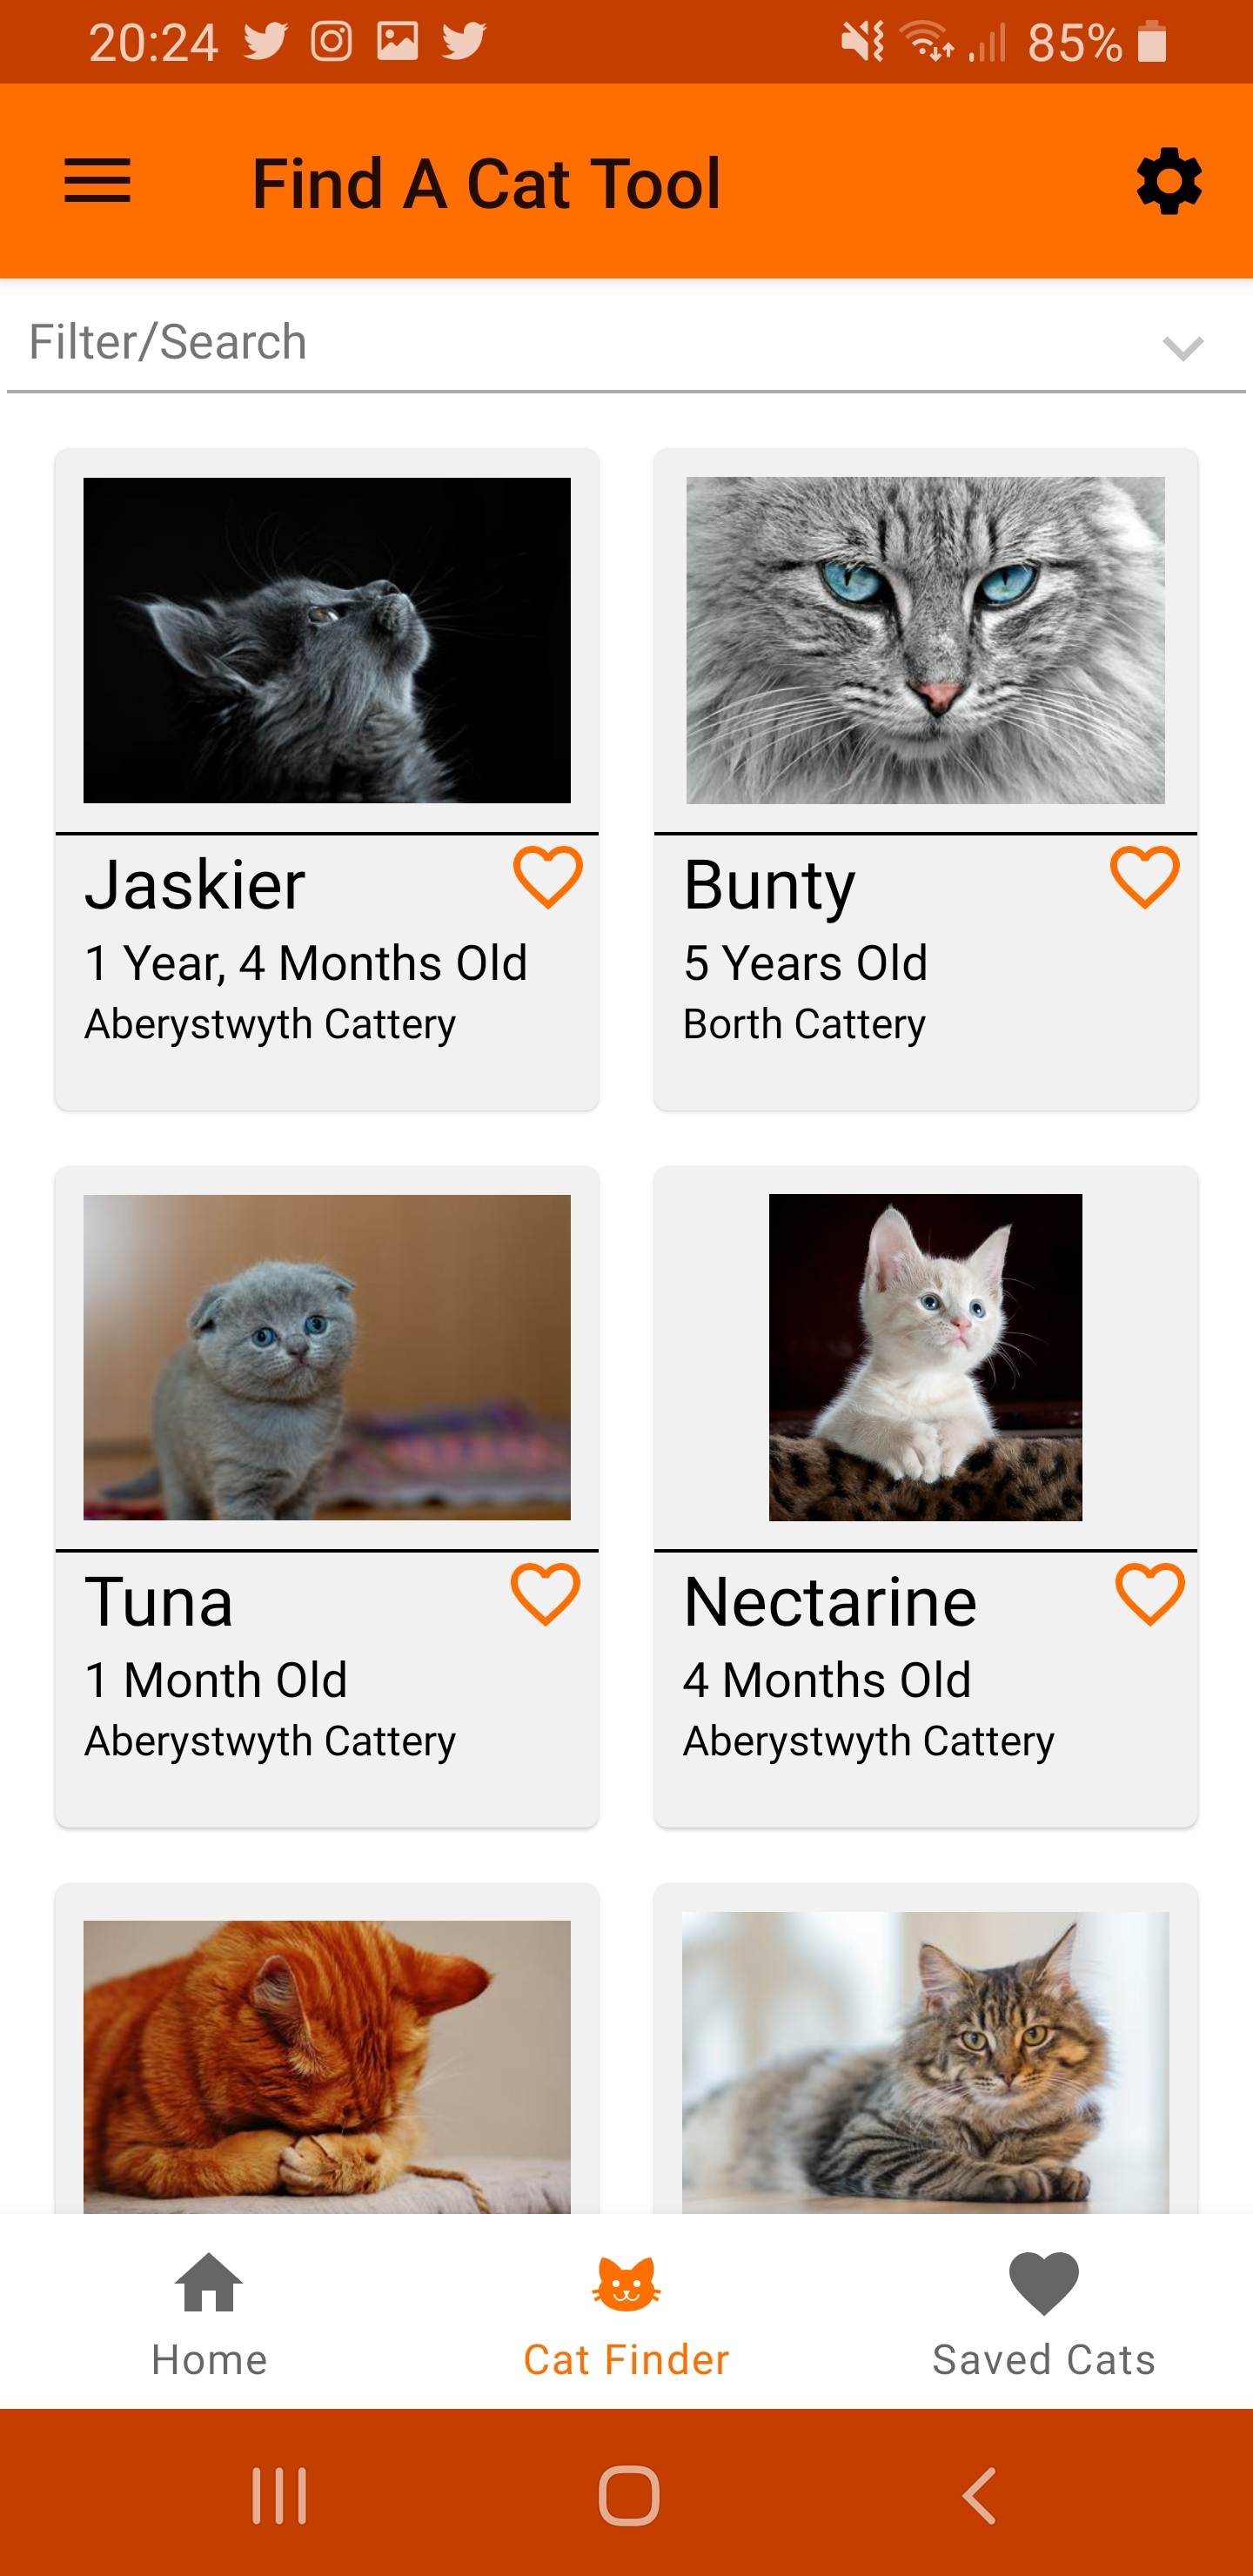
\includegraphics[height=7cm]{Images/CatFinderScreen.jpg}
    \caption{Implementation of Cat Finder}
    \label{fig:cat_finder}
\end{figure}

\begin{figure} [htbp!]
    \centering
    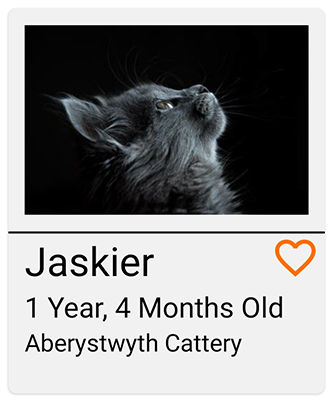
\includegraphics[height=3cm]{Images/CatCard.png}
    \caption{Cat card}
    \label{fig:cat_card}
\end{figure}

When implemented onto an actual phone the original prototype design didn't work, the text on the Cat \gls{Card} was too small, which made the layout unusable. To fix this, the Cat Card was enlarged, and it's content with it. The number of cat cards shown in a row was reduced to 2 to allow for the larger \gls{Card}s.

The Cat \gls{Card} layout also did not work very well in practice, in the prototype the favourite button was in the top right of the card over the image, this works if all images are white or transparent. Without a white or transparent background the icon could become invisible or hard to see, this lead to the slight redesign where it is on parallel with the name of the cat, it works the same as it did in the prototype.

\subsection{Saved Cats Card}

\begin{figure} [htbp!]
    \centering
    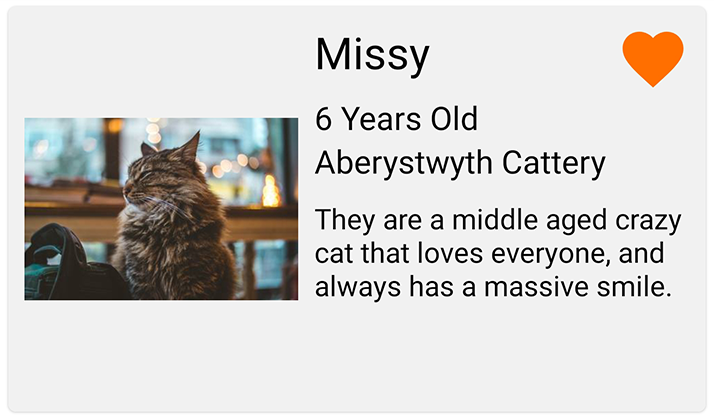
\includegraphics[height=3cm]{Images/SavedCatCard.png}
    \caption{Saved cat card}
    \label{fig:saved_cat_card}
\end{figure}

During implementation, it became apparent that the card was not designed to Material Design guidelines \cite{MATERIALDESIGNGUIDELINES}, the typical \gls{Card} in the guidelines has the image on the left, with the primary information and maybe a bit extra smaller near the bottom on the right side. To keep to this general guideline, I redesigned the Saved Cat \gls{Card}. This new layout should be quicker to glance at due to only needing the image to recognise which cat is which. This design flips if the user is using a right to left layout on Android.

\subsection{Adoption Confirmation Screen}

\begin{figure} [htbp!]
    \centering
    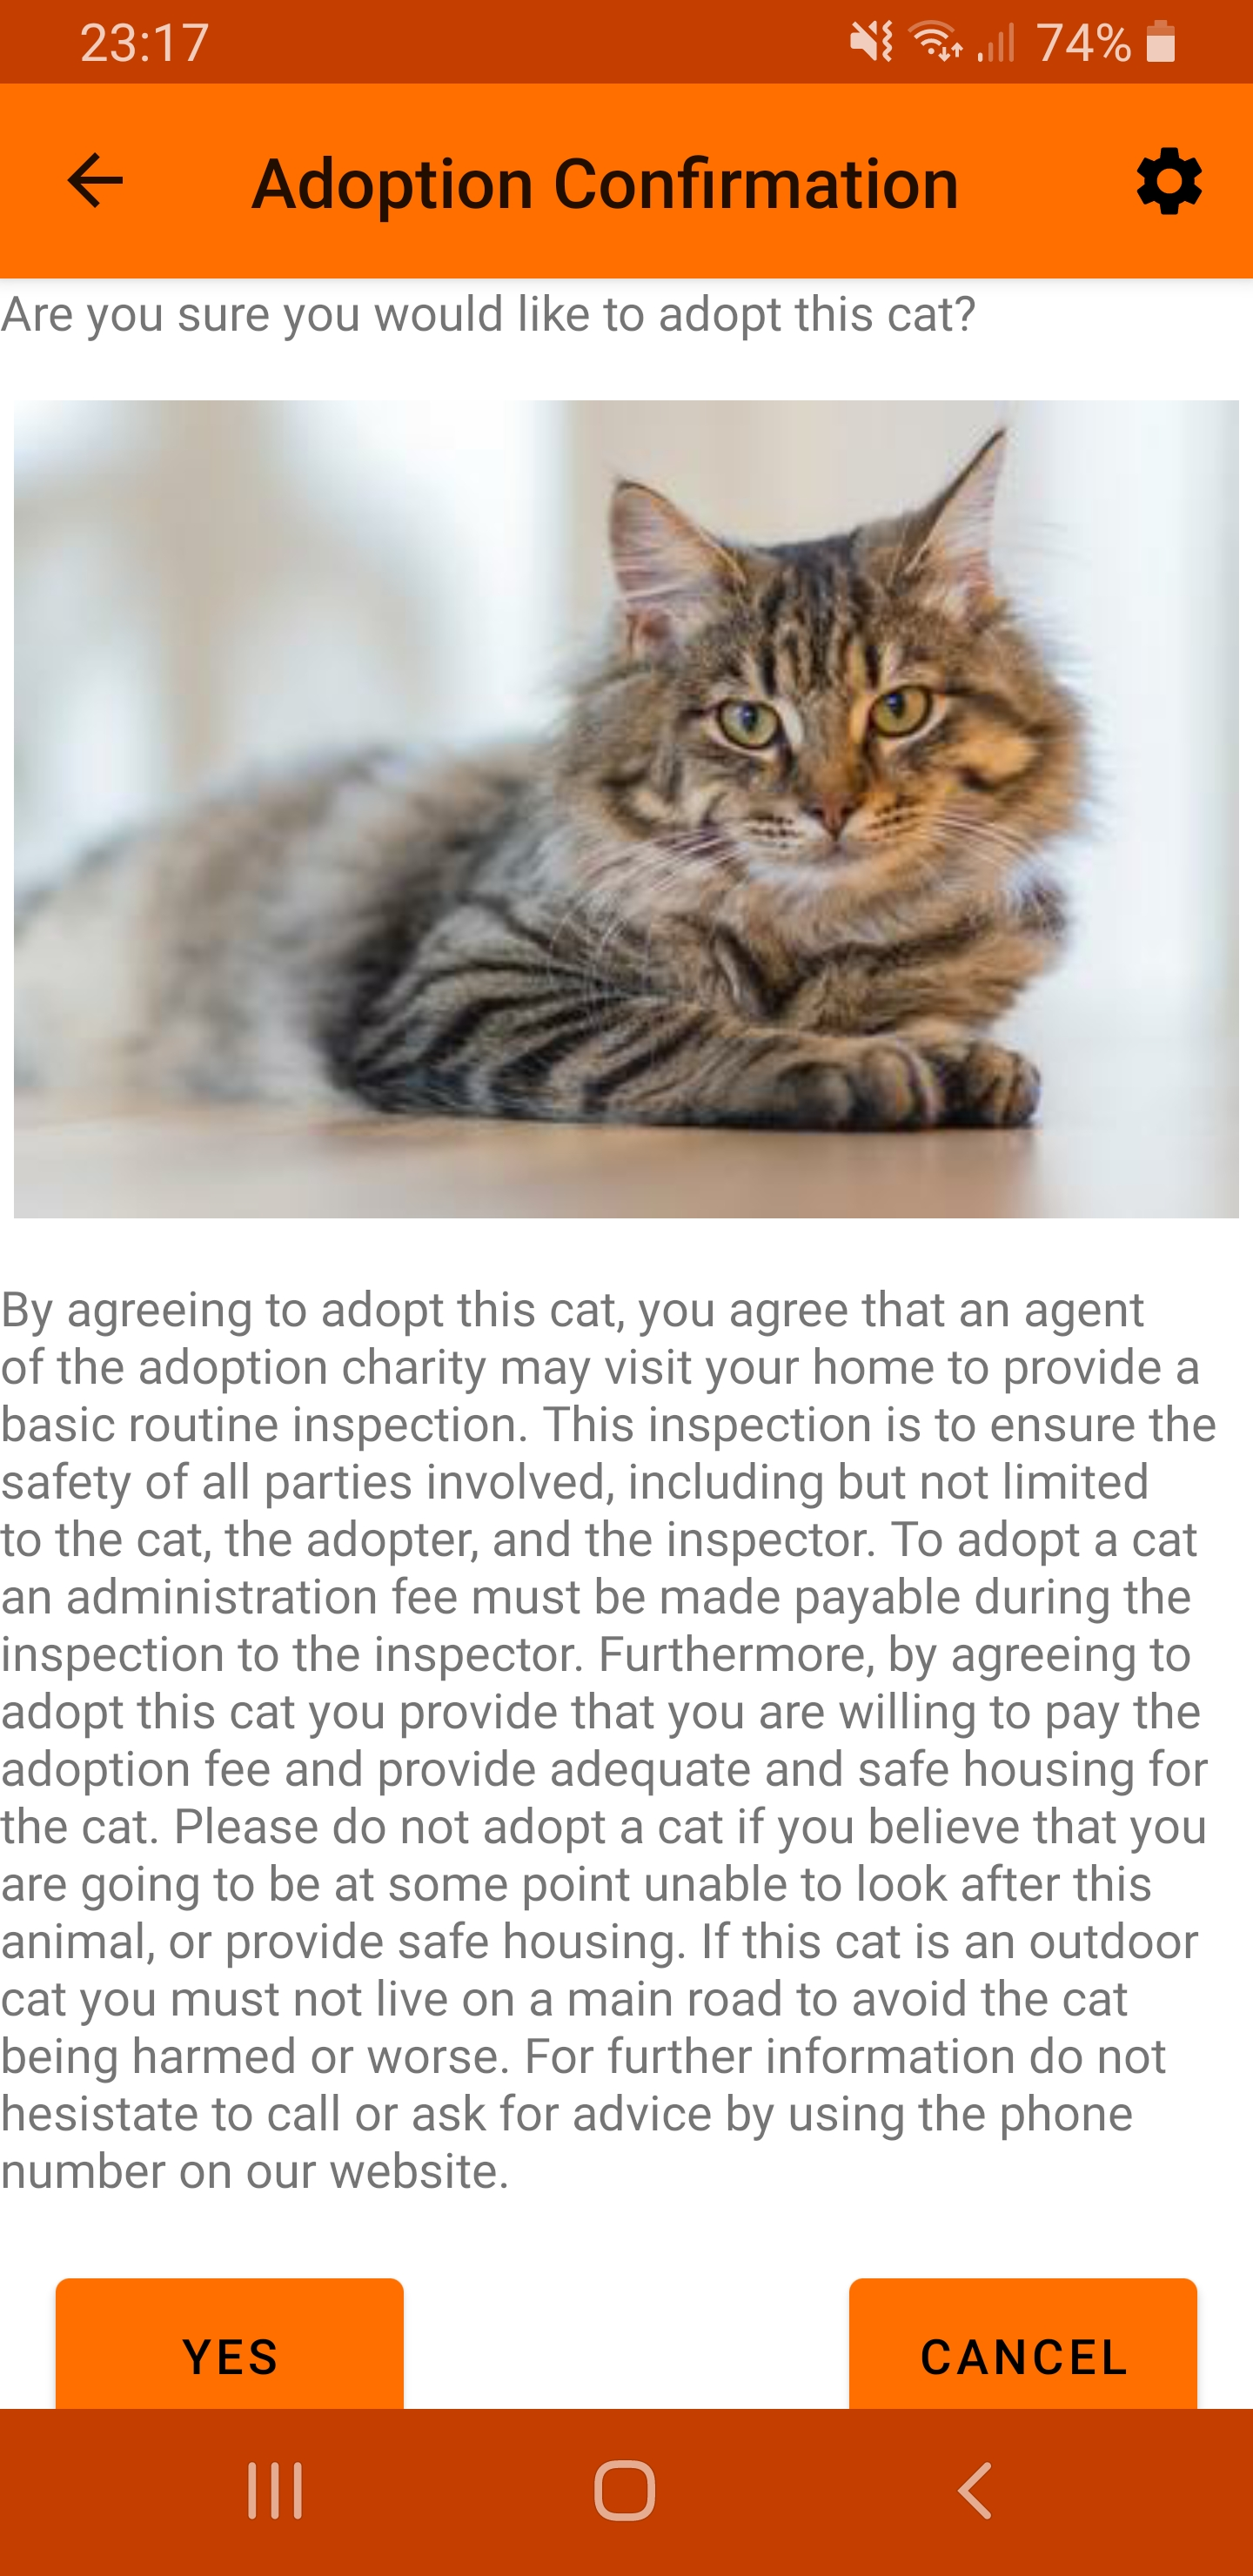
\includegraphics[height=7cm]{Images/AdoptionConfirmationScreen.jpg}
    \caption{Adoption confirmation screen}
    \label{fig:adoption_confirmation_screen}
\end{figure}

The adoption confirmation screen was added as a necessity to make sure a user is sure they want to start the adoption process. It was added later in the development process because of when clicking update on the information form that appears after being logged in and clicking adopt, it isn't apparent to a user that they have started the process necessarily. This screen adds some much-needed clarity, as once you click that yes button, you start the process, or by clicking the cancel button effectively cancelling the process.

\subsection{Settings}

\begin{figure} [htbp!]
    \centering
    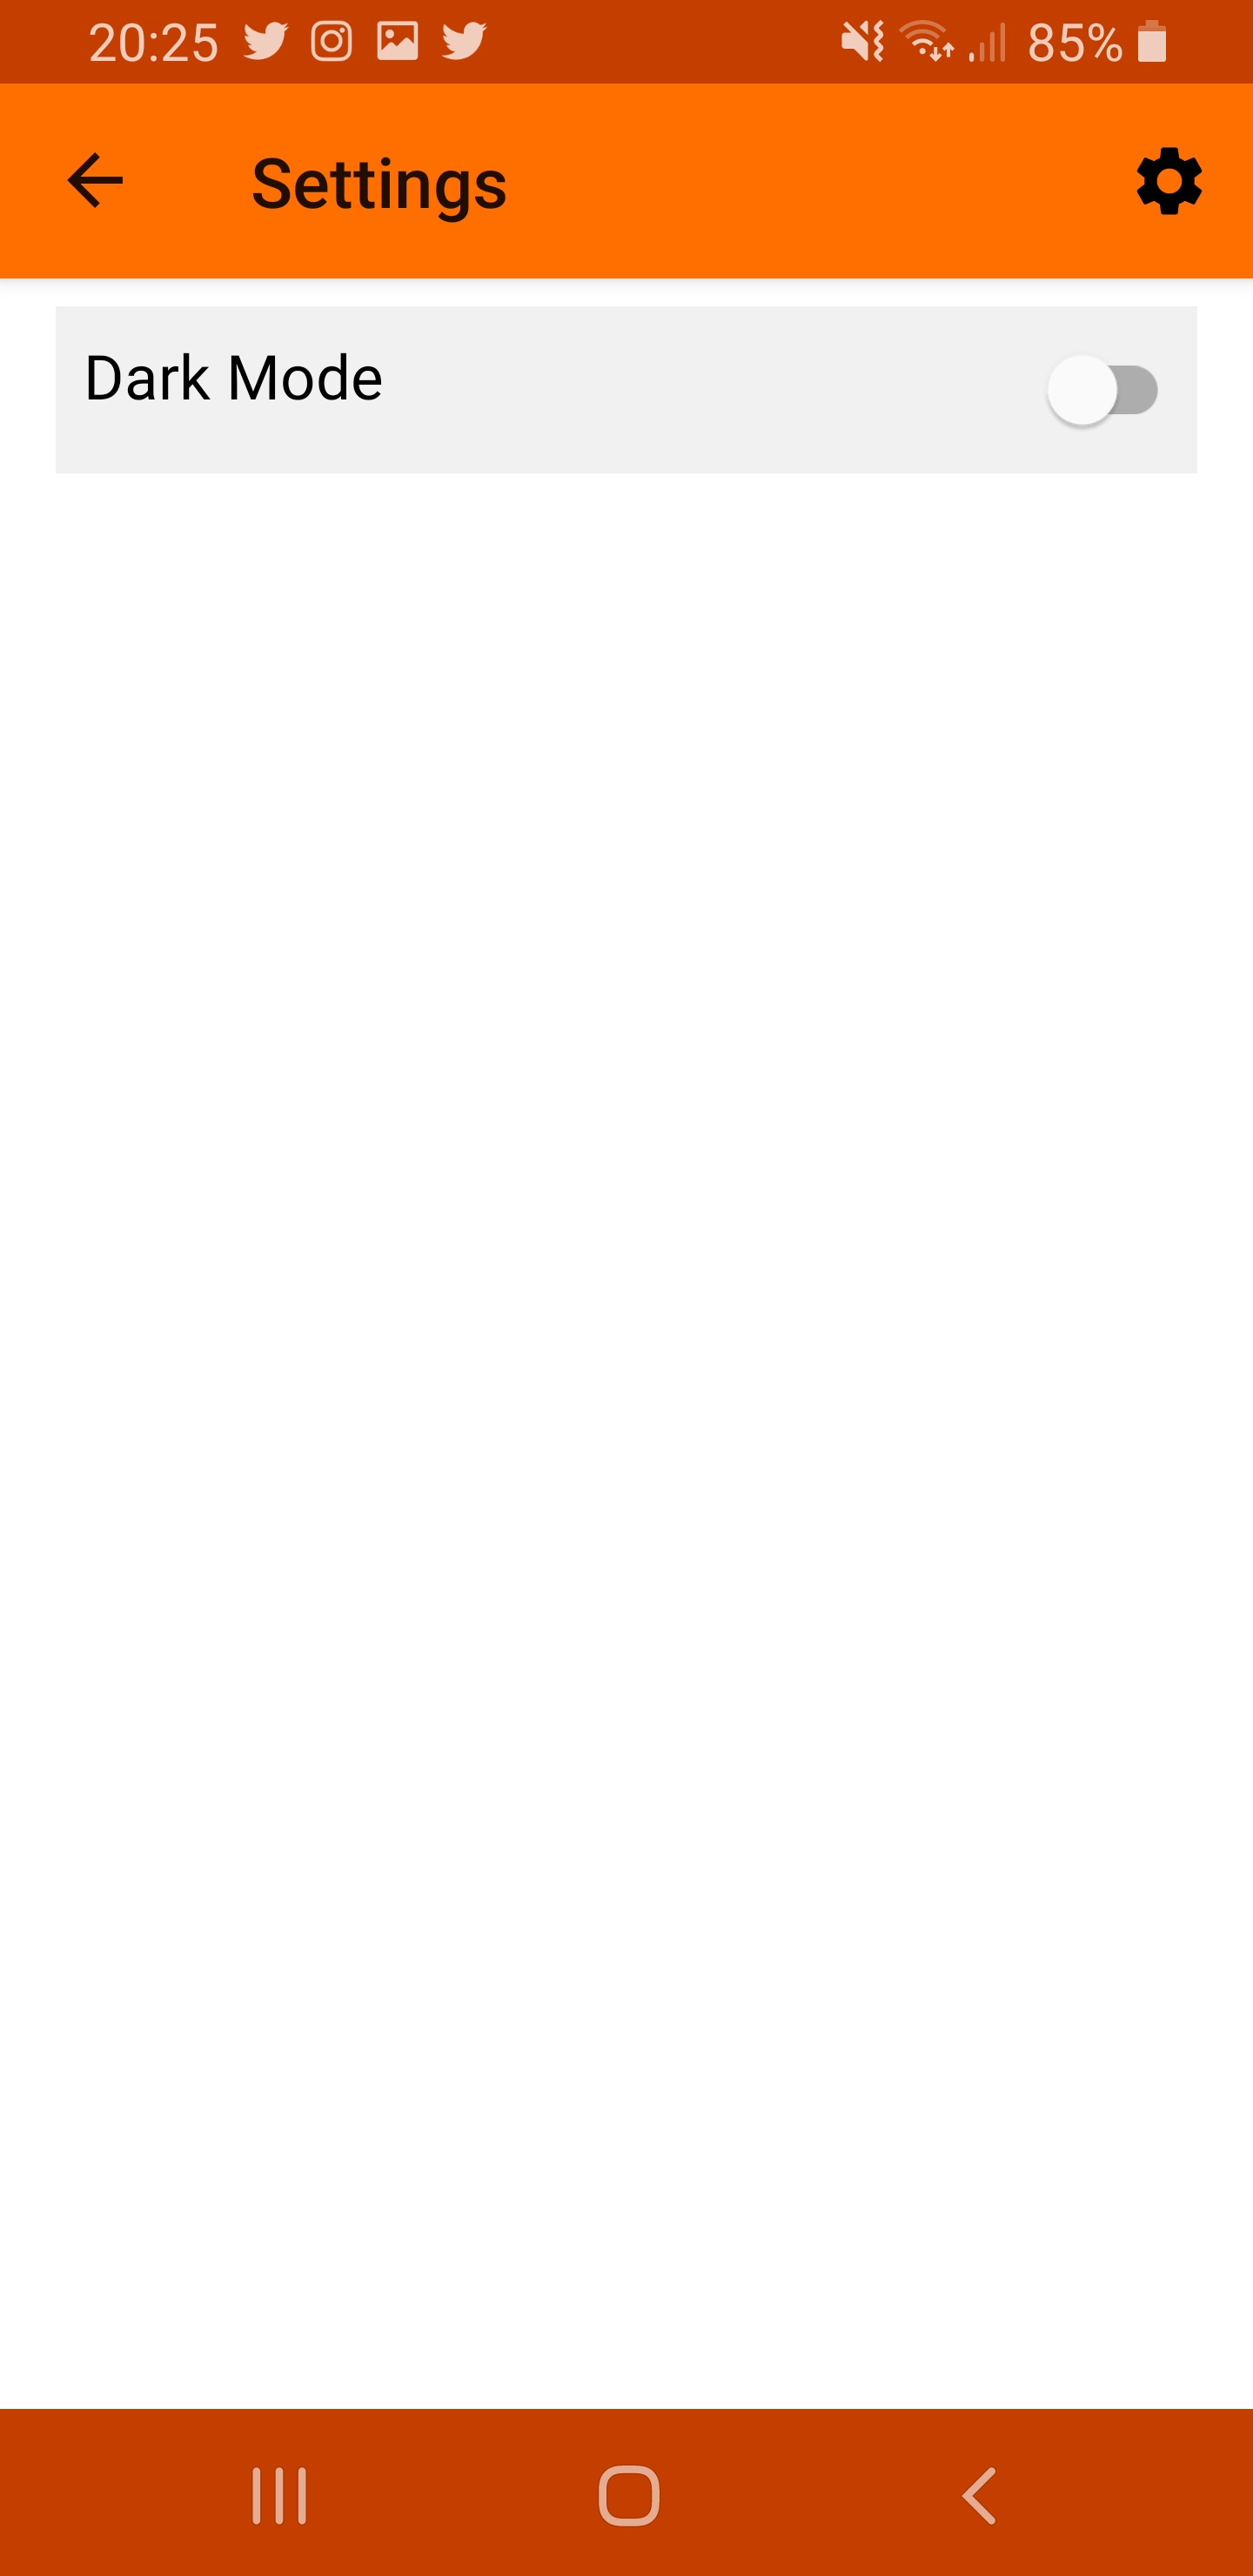
\includegraphics[height=7cm]{Images/SettingsScreen.jpg}
    \caption{Settings screen}
    \label{fig:settings_screen}
\end{figure}

The prototype settings menu contained a section for notifications, the final settings do not for two reasons, due to time constraints the notifications while present is not changeable from inside of the settings screen of the application. The second reason is, in more recent versions of Android it is possible to change these exact settings in the App info, it is also possible in all versions of Android to reject notifications from an application. 

While the prototype had green buttons, this did not follow the Material Design guidelines and was an oversight, so they were replaced to follow the guidelines with the correct colouring to represent the different states of the switches. The original prototype also had a cross instead of the up button on the upper left corner of the app while in the settings, this was switched to an up button in line with the Material Design guidelines for navigation.

\subsection{Navigation Draw}

\begin{figure} [htbp!]
    \centering
    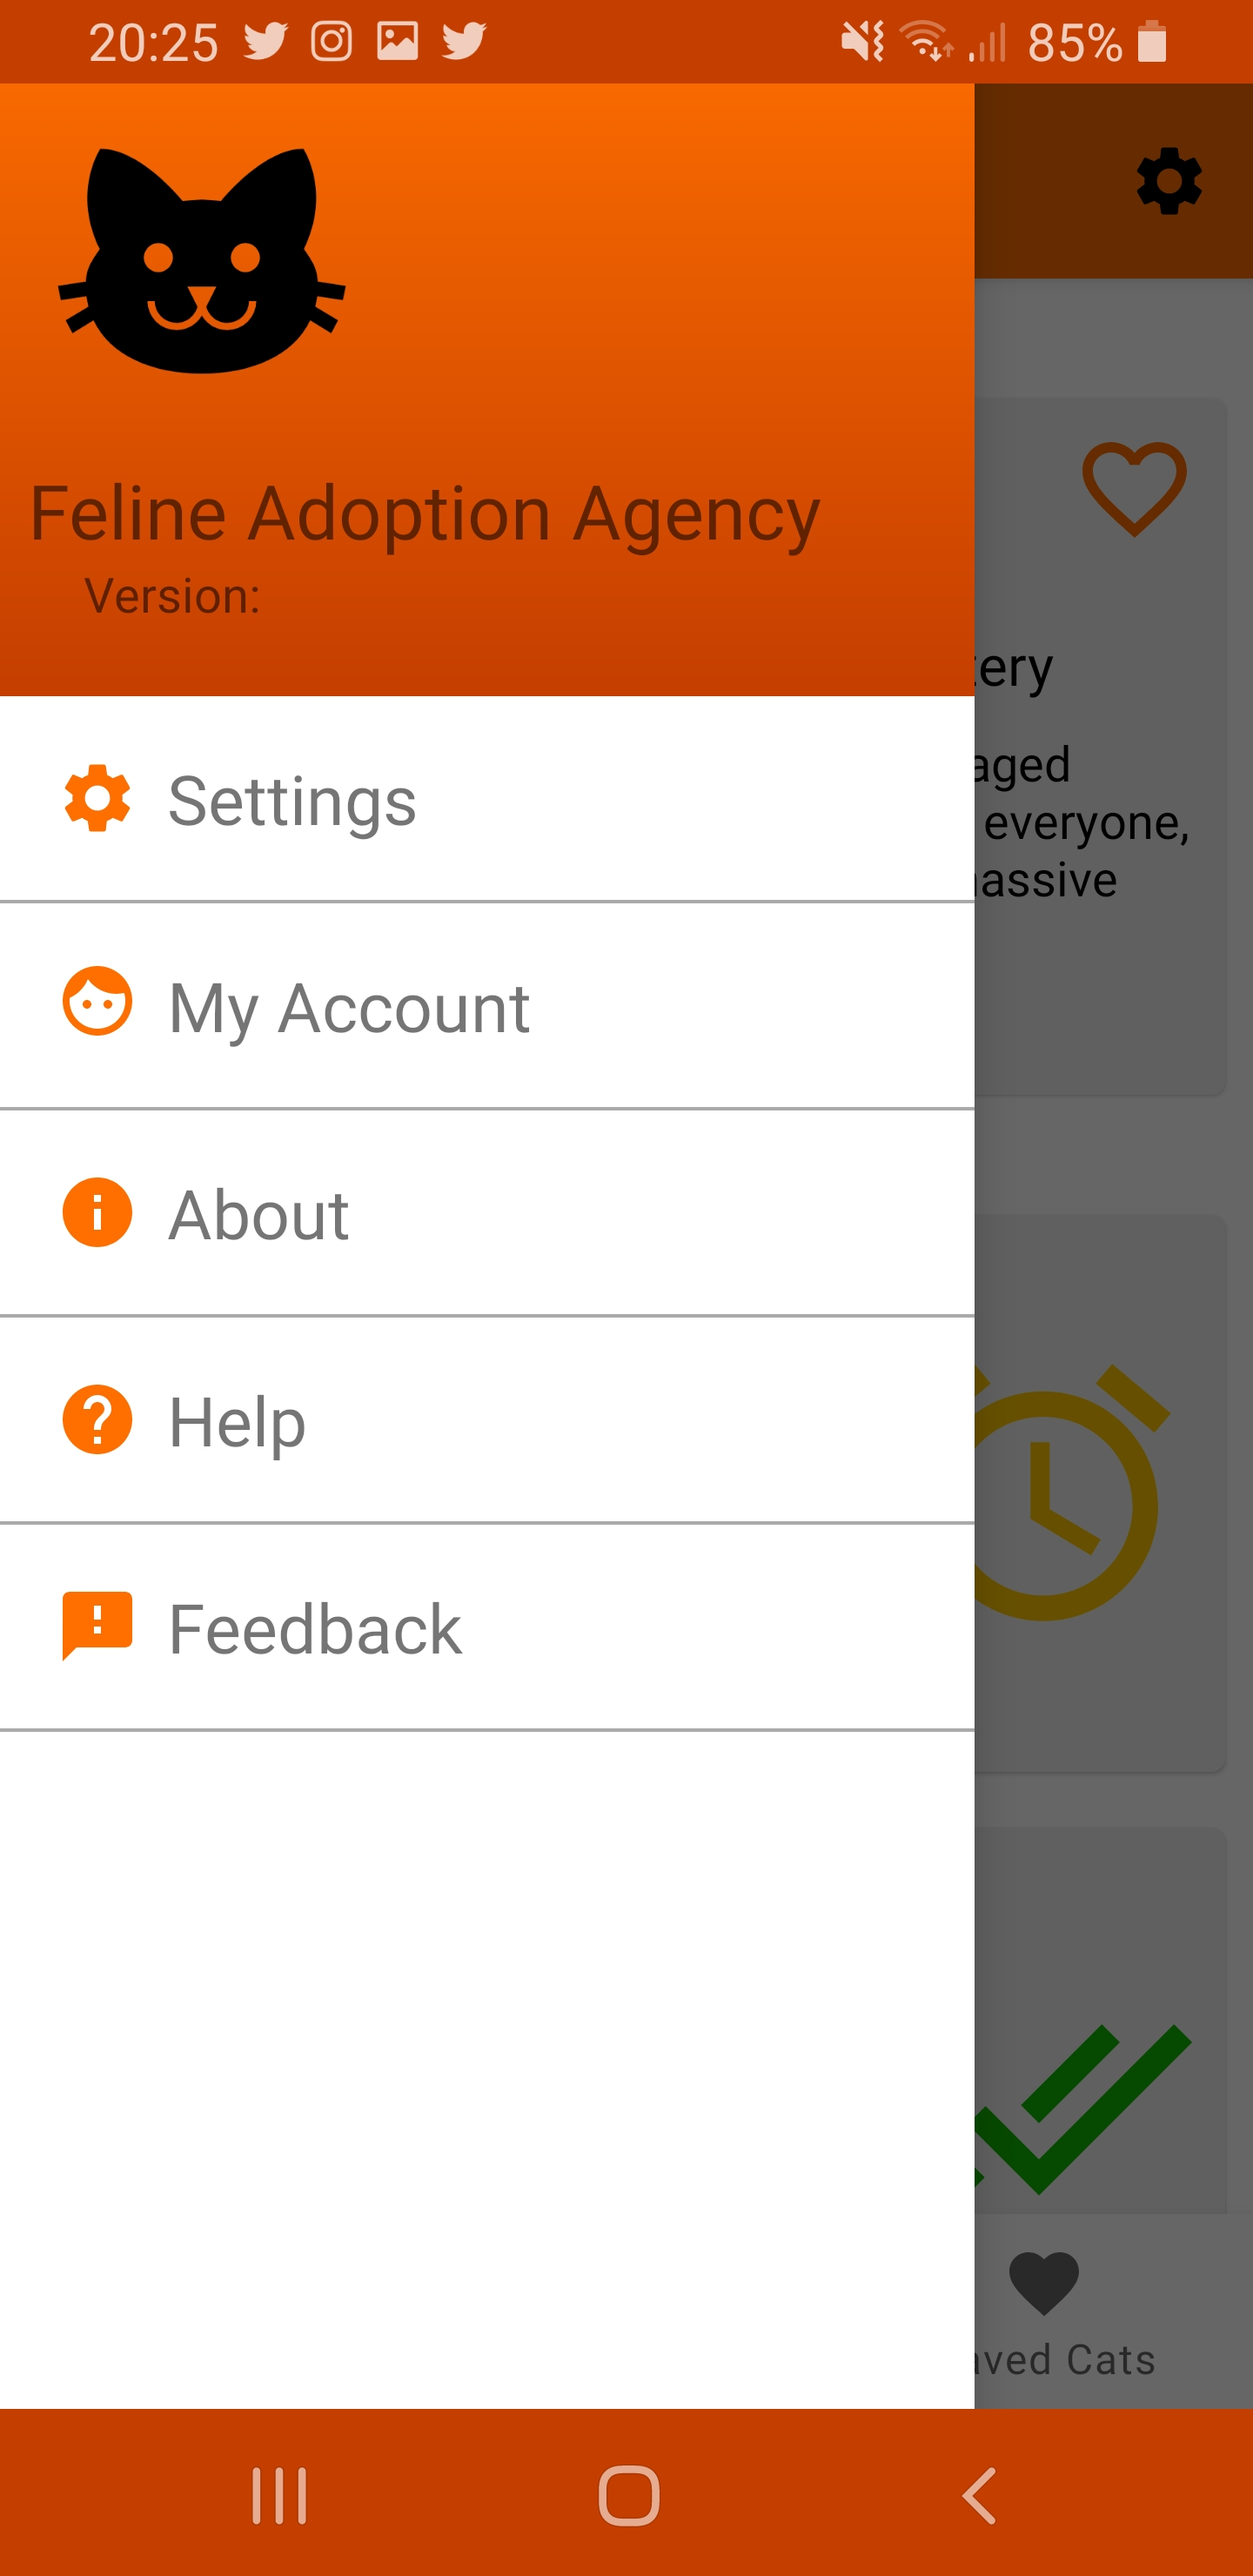
\includegraphics[height=7cm]{Images/NavigationScreen.jpg}
    \caption{Navigation draw}
    \label{fig:navigation_draw}
\end{figure}

The prototype navigation draw (Section \ref{PROTOTYPENAVIGATIONDRAW}) was never intended to be a final product or close to the final product. The final navigation draw (Figure \ref{fig:navigation_draw}) is a far superior design for multiple reasons, including the fact it makes more use of the primary colour scheme, it is interactive based on the state of the application (Login being replaced with My Account and a picture provided by the account logged in with), and it has a nicer header than just the logo that is shown in the prototype.

\subsection{Notifications}

\begin{figure} [htbp!]
    \centering
    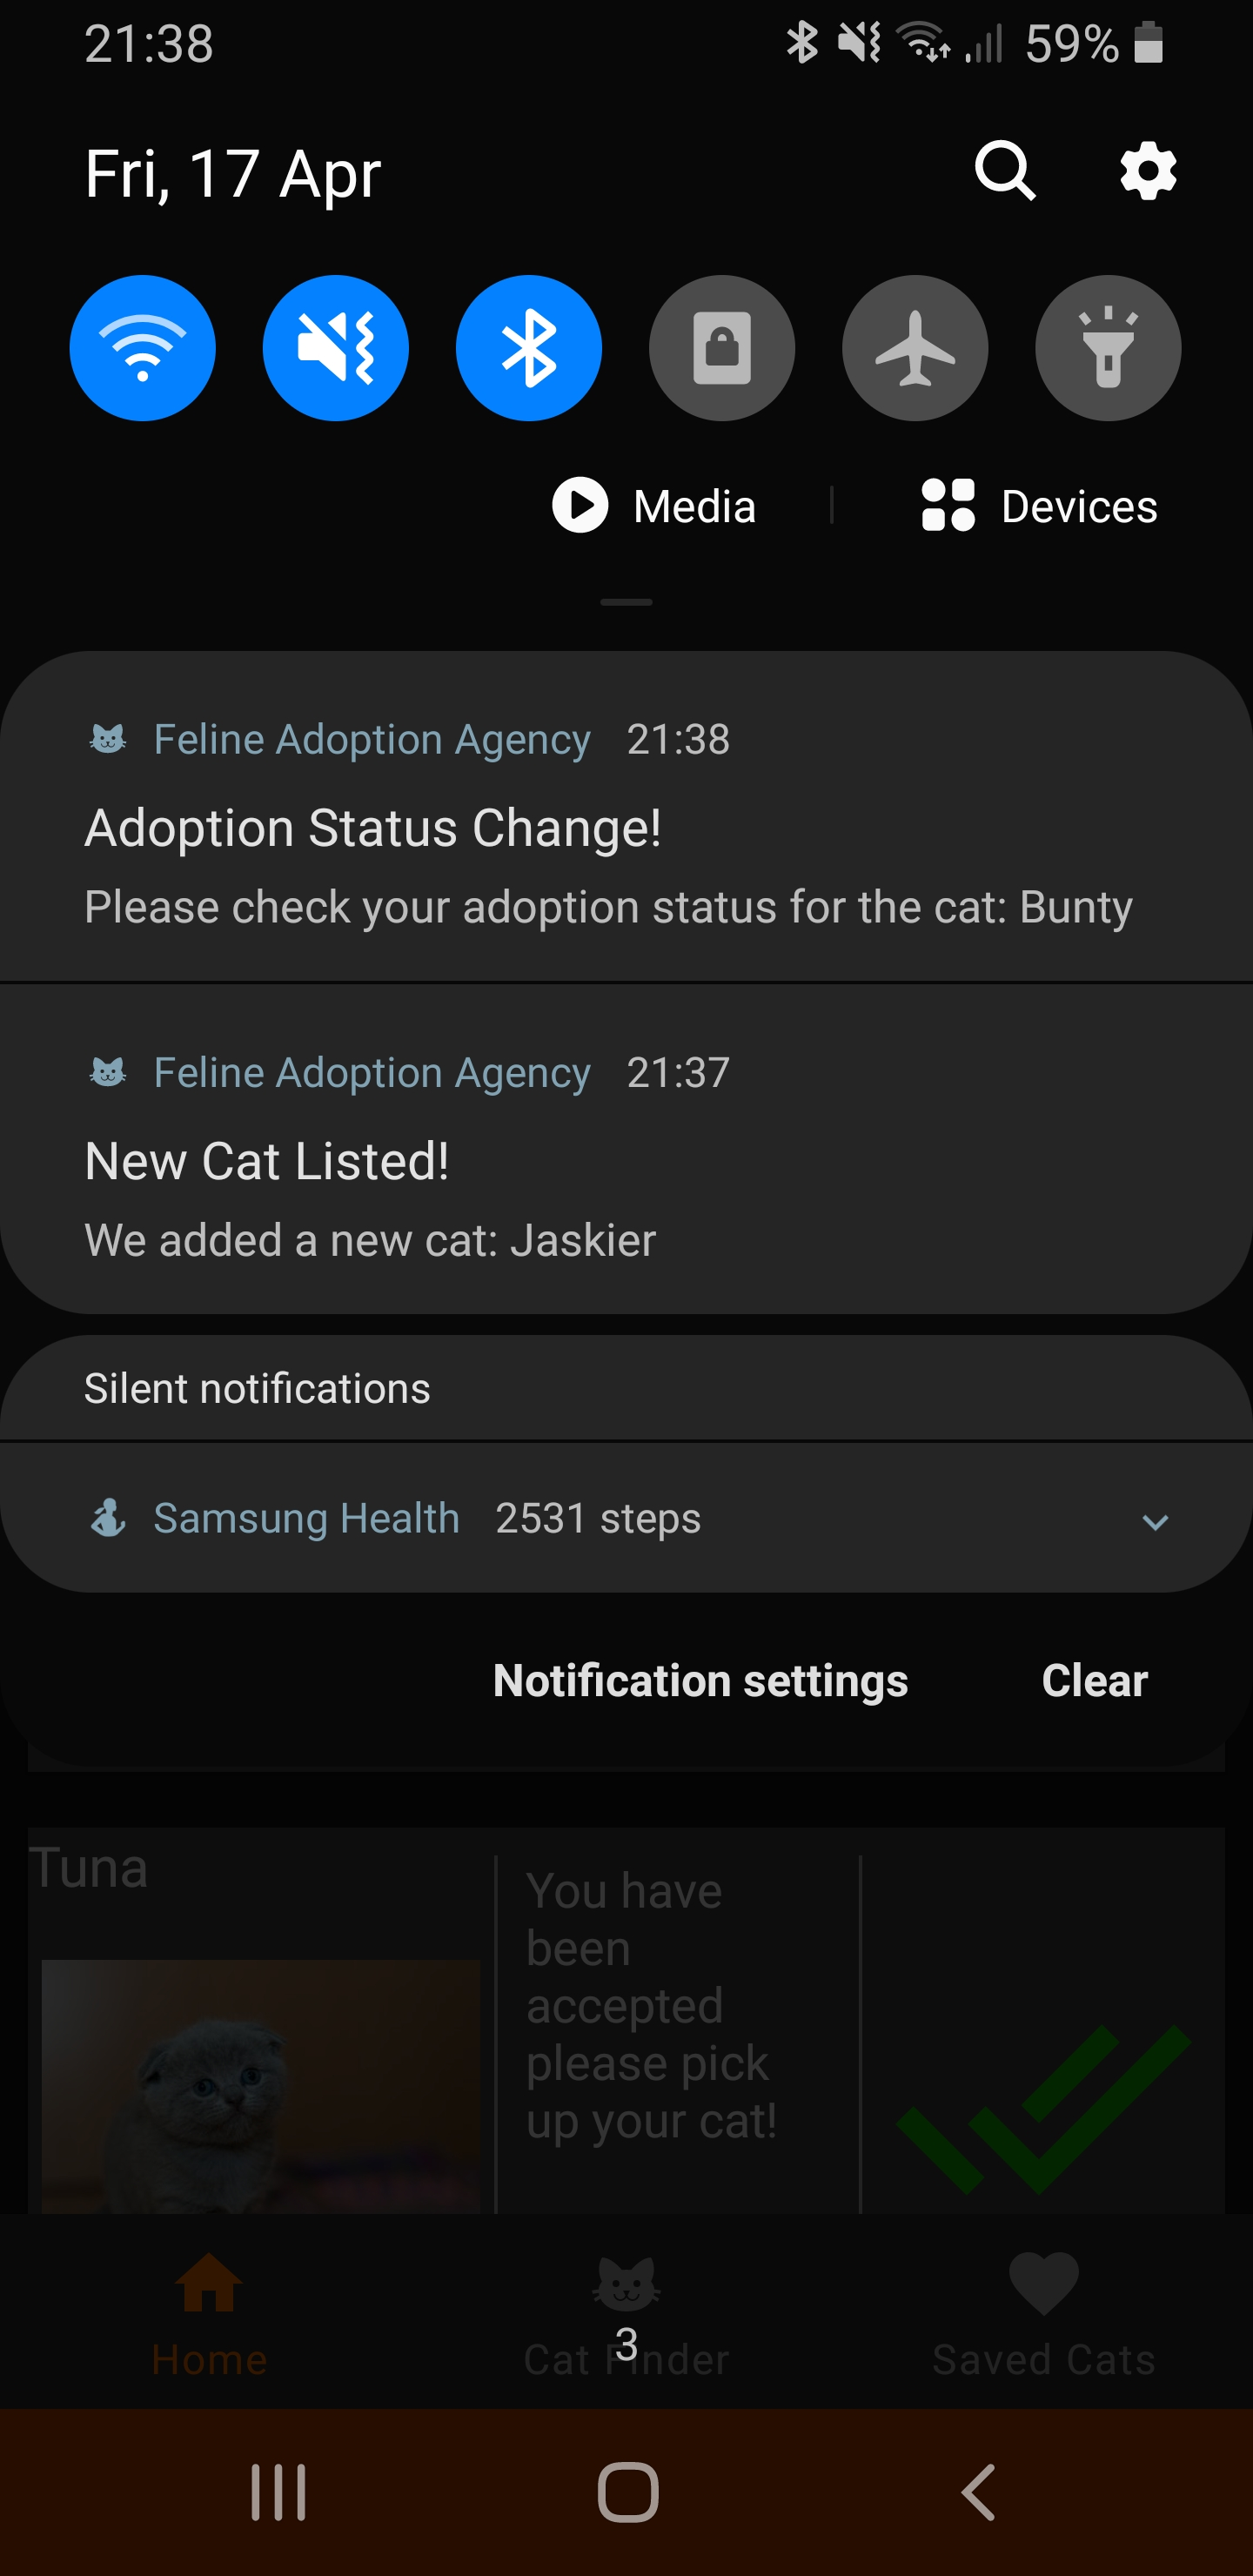
\includegraphics[height=7cm]{Images/Notifications.jpg}
    \caption{Notifications from the Feline Adoption Agency}
    \label{fig:notifications}
\end{figure}
The prototype never discussed how notifications would appear on a user's phone, and the basic Android notification pops up with a small image and with text,
 that is the exact implementation design that was completed, as shown in Figure \ref{fig:notifications}. Notifications pop up when a user's adoption status changes, a new cat is added, and some news from the agency is announced.

\section{Architecture} \label{CODESTRUCTUREDESIGN}

This section is an attempt at explaining to the reader how the UI Design and the code inside of the application fit together. Furthermore, this chapter goes into detail about how different components of the application fit together and what components there are.

\subsection{Overall Architecture}

The overall architecture of the application revolves around the theory of one activity, many fragments, this is the preferred method of application implementation \cite{SINGLEACTIVITYAPP}. The main application relies on Android Jetpack NavigationUI \cite{NAVIGATIONUI}, to navigate between fragments in the application. It is possible to pass a Java Parcelable object between fragments for data transfer, during navigation.

    \begin{figure} [htbp!]
        \centering
        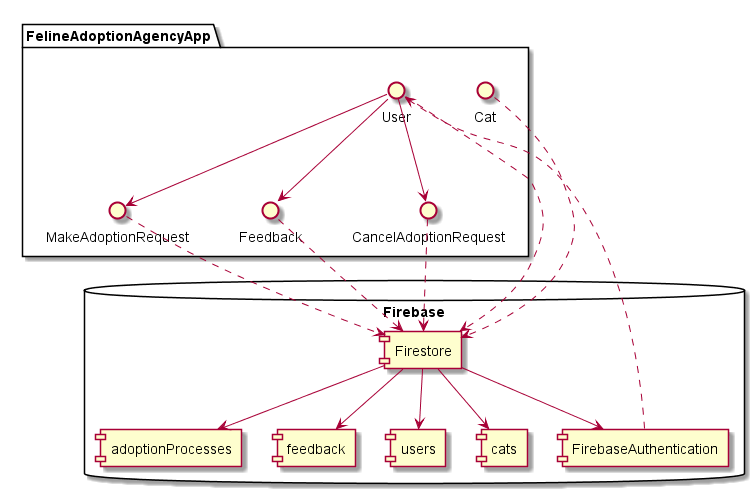
\includegraphics[width=\textwidth]{Images/ComponentDiagram.png}
        \caption{UML Component Diagram}
        \label{fig:component_diagram}
    \end{figure}
    
So far, we have not thought about how data gets to and from the application. For this, I intended to use Google's Firebase Firestore for databases using a NoSQL structure with JSON files, Firebase Authentication for authenticating a user's identity and storing of user account identifiers, and Firebase File-storage for storing pictures of cats at a URL location so the application over the internet can load them. Figure \ref{fig:component_diagram} displays the rough interactions between the app and the Firebase, inside it has the Firestore, which is the database, and the authentication of users.

    %Sequence Diagram should be added
    \begin{landscape}
        \begin{figure} [htbp!]
            \centering
            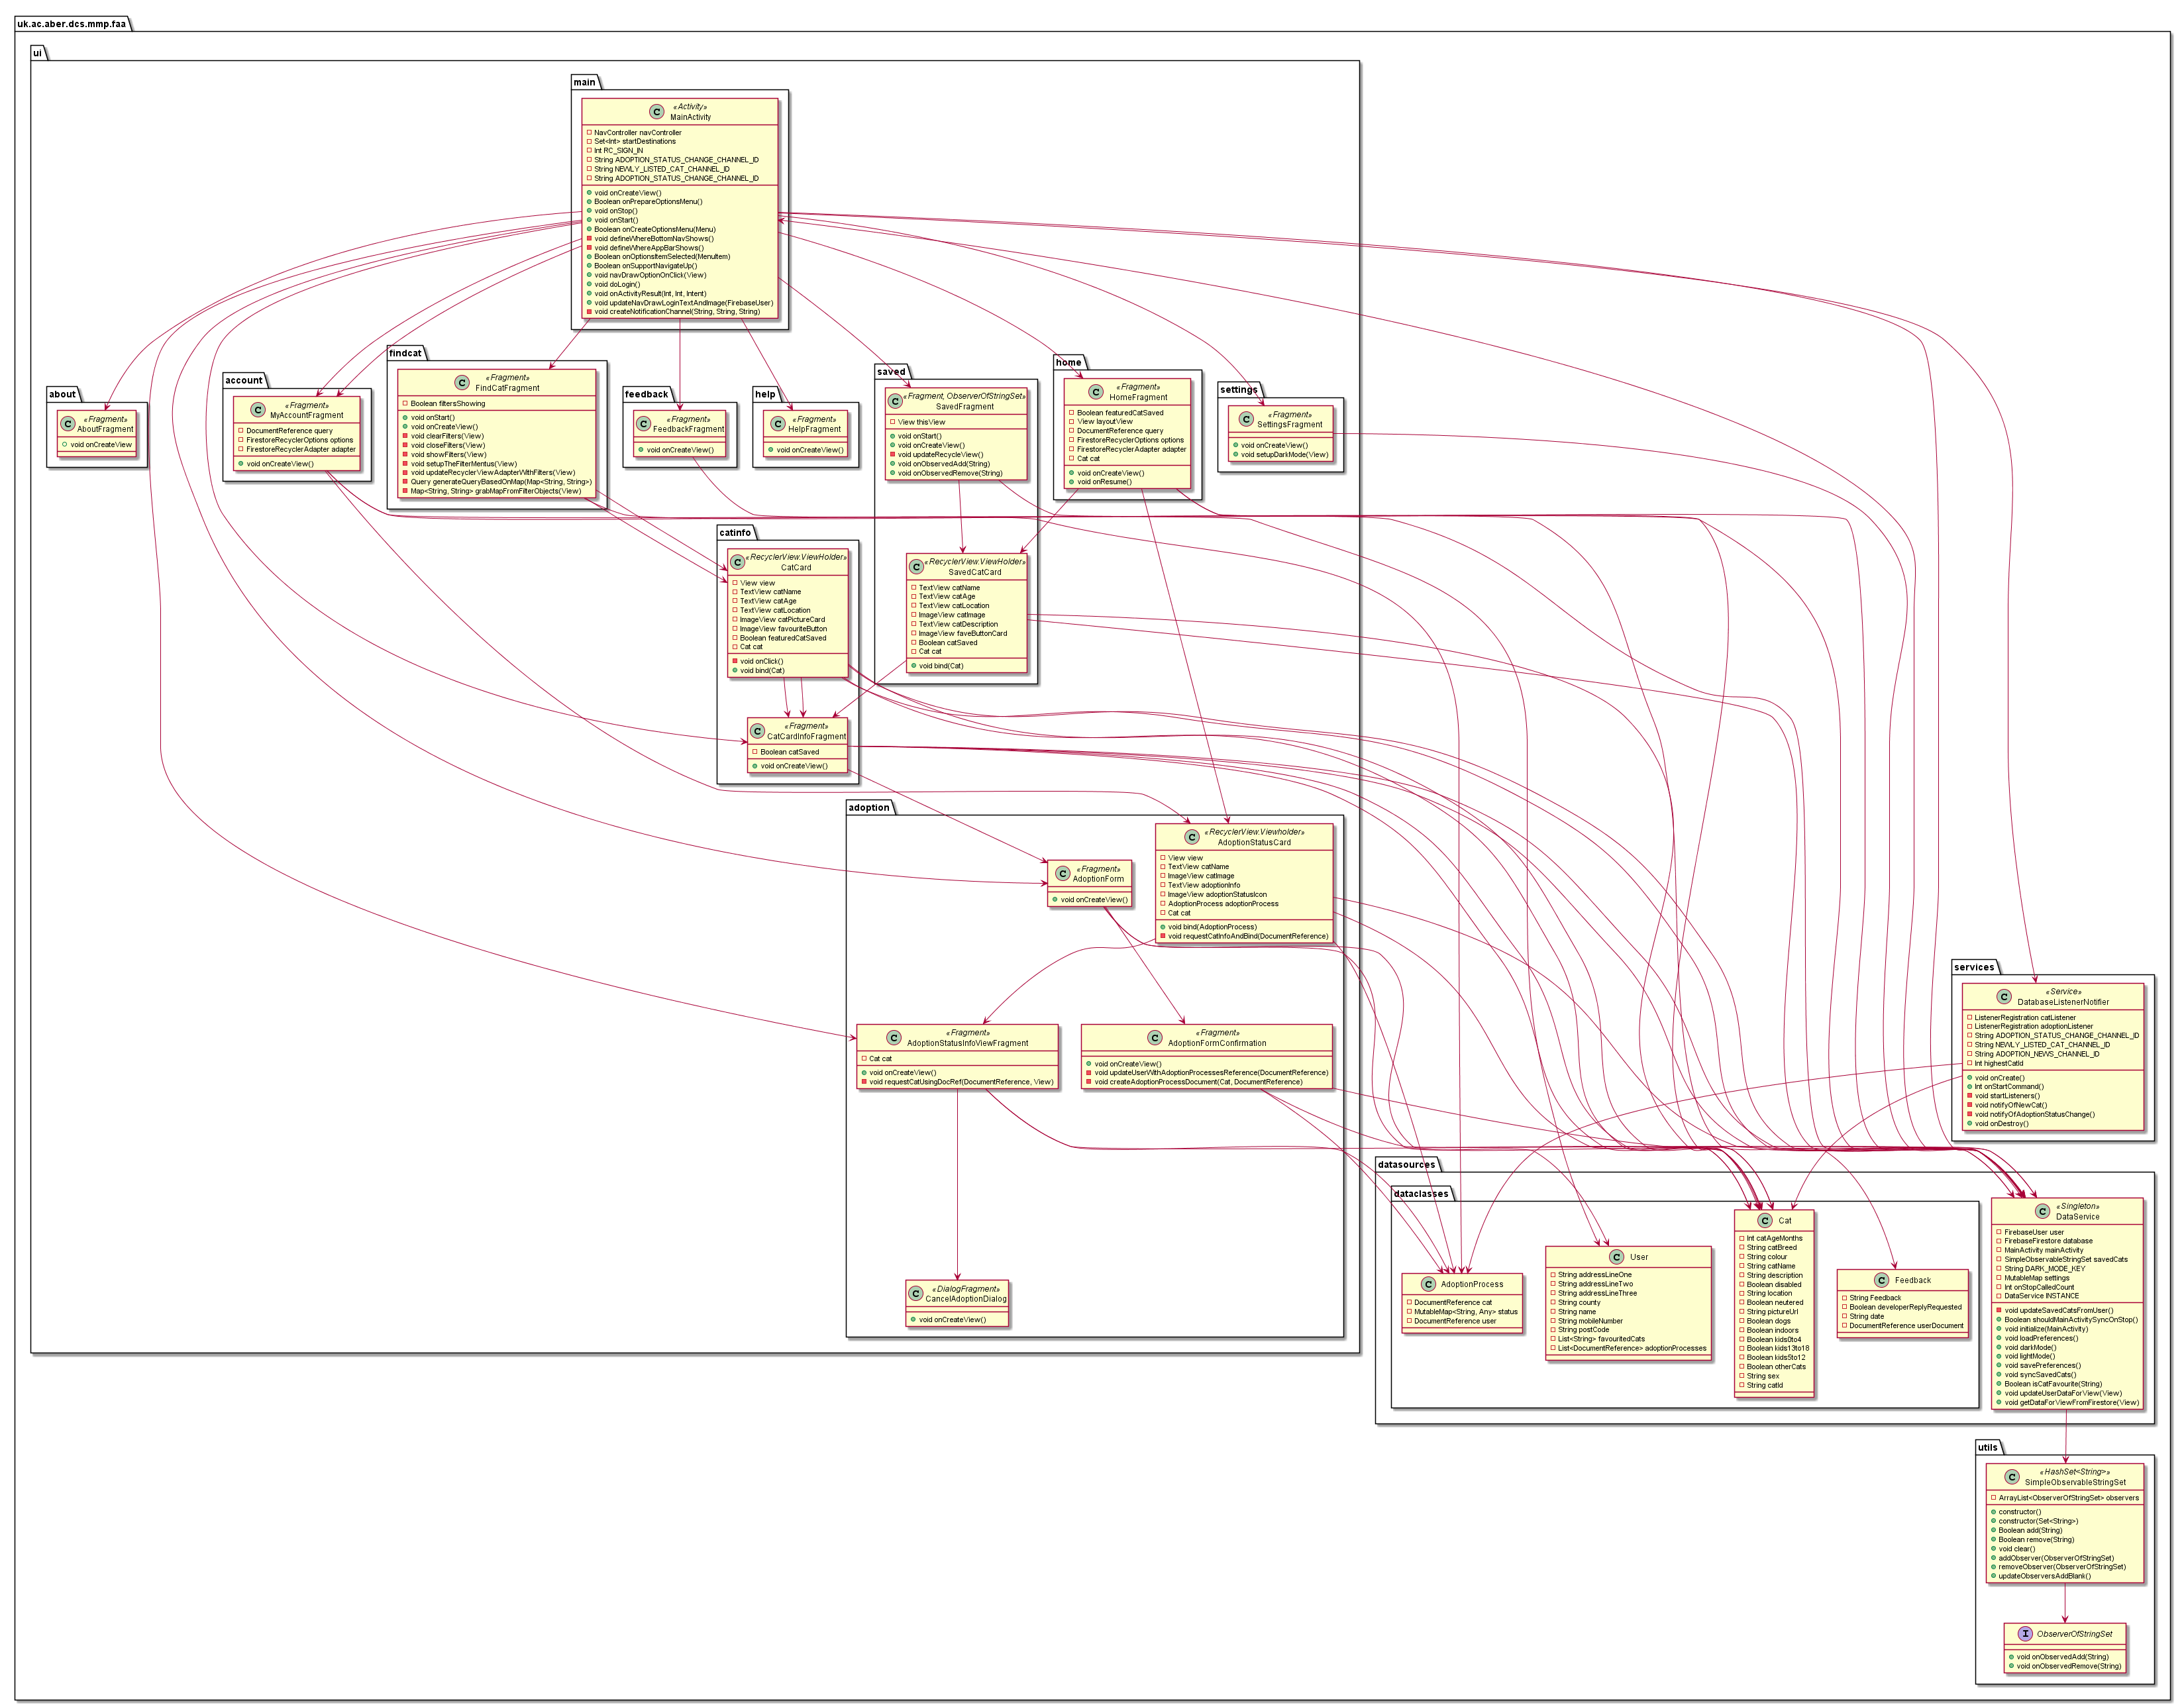
\includegraphics[scale=0.18]{Images/ClassDiagram.png}
            \caption{UML Class Diagram}
            \label{fig:classDiagram}
        \end{figure}
    \end{landscape}
    \subsection{Code structure}
    
    To show how the application's various classes fit together, I created the UML class diagram shown in Figure \ref{fig:classDiagram}. The application has various classes that all interact with each other, while classes are separated into packages ensuring more straightforward navigation in the project and separation of classes that have less in common with each other. To demonstrate the separation of packages look at the package under UI called adoption, it contains all UI elements that are concerned with the adoption process. 
    
    Many classes make use of the data classes which contain Cat, AdoptionProcess, User, and Feedback classes, where possible these classes are based on a Kotlin Data class, where it's explicit purpose is just for data storage, there is no particular need for these classes to do anything but that, it may be required however for some dataclasses to implement the Java Parcelable interface. Parcelable is required to transfer these data classes to the fragment that is being navigated to.

\subsection{DataService}

The DataService is a crucial part of the application, I have found through personal experience that using a central place for data retrieval throughout the application's UI elements allows me to cut down on spaghetti code and replace it with an interface that allows the UI to be interchangeable; This allows the data provider to be interchangeable, it's aim is to implement the role of the Presenter in a Model-View-Presenter relationship in GUI design \cite{MODELVIEWPRESENTER}. Due to the nature of the project, Google Firebase became a more vital interface and such in the project we have 2 DataServices, the local version for all data tracking not done with FirebaseFirebase, and the database reliant parts were done with the Firebase Firestore equivalent.

The DataService can be used by any of the parts of the application to call for a login request, and this is due to the nature of the DataService being initialised and owning a reference to the MainActivity, this is used throughout the application where being logged in is required to perform specific actions. The depth to which the DataService class is used is highlighted during the sequence of events that take place in the adoption process shown in the UML Sequence Diagram in Figure \ref{fig:sequenceDiagram}.

The DataService functionality is primarily inspired by the AnalysisDataService, which is an implementation of a DataService \cite{MANTIDDATASERVICE} class from the project I worked on during my Industrial Year, which held application-wide data for retrieval by individual interfaces.

        \begin{figure} [htbp!]
            \centering
            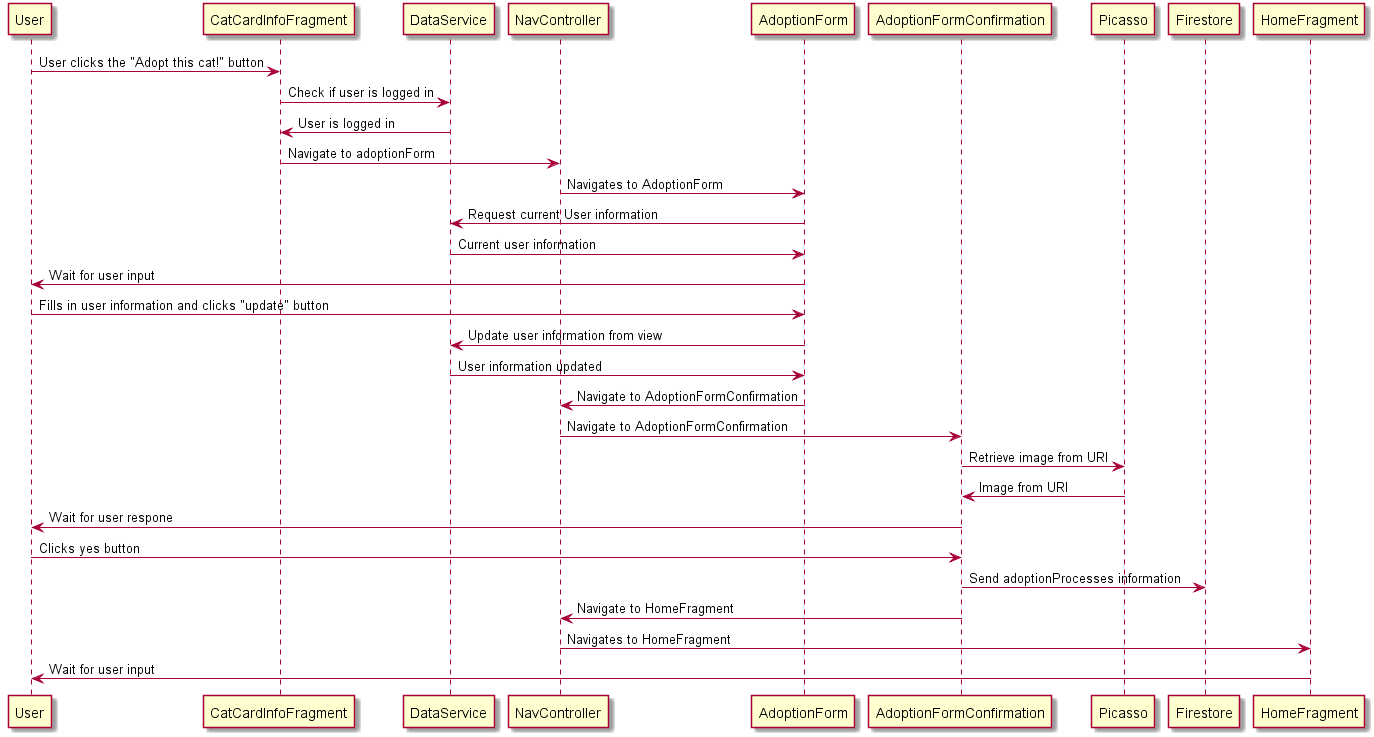
\includegraphics[width=\textwidth]{Images/Sequence Diagram Adoption Button Click.png}
            \caption{UML Sequence Diagram for adoption button being clicked}
            \label{fig:sequenceDiagram}
        \end{figure}
\subsection{MainActivity}

Due to the nature of a one Activity many fragment Android application, some significant functionality must be implemented in the aptly named MainActivity. The name is accurate as it is my only Activity. It is not the only Activity in the application, but the only one directly created by the project as Firebase Authentication runs in a separate activity. 

The MainActivity handles, the creation of the Navigation Draw, \gls{Bottom Navigation Bar} and it's configuration, Navigation Controller, Logging in, Notification Channel creation, and the application bar and its configuration. Parts of the MainActivity where it handles configuration is where these items are displayed, for example, the \gls{Bottom Navigation Bar} is only shown in main locations of the app, these are the HomeFragment, CatFinderFragment, and SavedCatFragments.

All Activity related Android lifecycle elements and primary setup and initialisation must occur in this one class, to stick to the One Activity, Many Fragments \cite{ONEACTIVITYMANYFRAGMENTS} methodology that is implemented in so many modern applications. 

Multiple activities require in some cases up to 2x CPU usage. On mobile devices, CPU is a limited resource and thus reducing CPU usage is key to a fast and smooth running device and application. The reason multiple activities require increased CPU usage is due to the nature of Activity creation and destruction on Android as data is regenerated un-necessarily when creating more Activities \cite{ONEACTIVITYMANYFRAGMENTS}. This decreased CPU usage is at the cost of a small increase to memory usage; almost all modern phones have enough memory for this not to be noticeable. With the added benefit for a developer having greater control over the application, with simple interfacing with the navigation controller using NavigationUI \cite{NAVIGATIONUI}, it is a superior method of Android application implementation.

\section{Accessibility} \label{ACCESSIBILITYDESIGN}
In the modern-day, it is increasingly hard to socially interact and perform specific tasks without a mobile device; this, however, is not accessible to a large portion of the population without particular adaptations. For example, if someone is unable to see the smaller text on a small device, they may use a tablet, having your interface increase in size to that of a table would allow a user to see things that they couldn't otherwise. In this section, a discussion takes place for the design decisions that have been taken to adhere to the accessibility of people to this application across need barriers. Android already has many accessibility features built-in, and there is a set of guidelines to follow to best assist in their functionality \cite{ACCESSIBILITYPRACTICES}.
    \subsection{Text Size}
    The size of text should scale to the size of the screen using it, and this doesn't inherently happen in Android applications. Historically developers would use point size to discern the size of the text in their layouts; however as Android has been updated, it has introduced scale-independent pixels which scale with the size of the screen a user is using, alongside layouts that are designed to do the same. It is planned to implement scale-independent pixels for all text in the application. It is currently not completed.

Android offers the ability however to enlarge all text across all applications inside of its accessibility settings, so this feature was pushed down the road, as it is possible without specific support to users who understand the features available in the settings.
    \subsection{Layout Scalability - Tablet Support}
    I have tested that the app works on a tablet, it is functional however it does not look as sleek as on a mobile phone for which this application was designed, but it is functional and combined with built-in Accessibility features in Android such as display scaling looks much sleeker. There is a plan to support this more extensively without the need to utilise Accessibility features built into Android as people may struggle to find those in the first place, however, the breadth of this implementation is time-limited.
    \subsection{Start to End support throughout}
    To support many locations across the globe, modern Android has implemented start to end layout opposed to left to right, and this provides support for people in areas that use right to left in literature as it may make it easier for users from these areas to more easily adopt Android. To support start to end layouts, all layouts in the application are created using Start to End implementation instead of left to right implementation. To increase user base and usability for users with a right to left layout, this accessibility is both easy to implement and vital.
    \subsection{Content Description for images}
    For people who are blind or hard of sight, it is important to provide a content description for all images, this is encouraged in Android Studio and is also simple to implement in multiple languages for internationalisation using strings. Content descriptions are read using computer-generated voices to users who are blind or hard of sight, much like the text is read, this is a feature baked into Android itself, but the application has added extra support for this in the form of the Content-Description for images.
\chapter{Implementation} \label{IMPLEMENTATION}

\section{Firebase Configuration} \label{FIREBASECONFIGURATION}
    \subsection{Firestore Structure} \label{DATAIMPLEMENTATION}
    Each of the 4 data classes in this application is represented by a JSON file in the file structure of the Firestore. The 4 data classes are represented in the application by either a Kotlin Data Class \cite{KOTLINDATACLASS}, or a data class like a class with some additional methods for Parcelable functionality. The files are set up in a certain structure for the data to be retrievable using these classes. The idea is that each of the fields in the JSON files is represented by 1 variable in the data classes if the JSON file has a string, then a string with the same name as the JSON variables key is used in the data class. For example, a JSON file that looks like this:
    
\begin{verbatim}
    {
    "name": "MyName"
    "age": "MyAge"
    "location": "Location"
    }
\end{verbatim}
    
    Is accessible as a data object in Kotlin formulated like this:
    
\begin{verbatim}
    data class user(
        var name: String? = "",
        var age: String? = "",
        var location: String? = ""
    )
\end{verbatim}

    Data class examples can be found in the Appendix Section \ref{DATACLASSEXAMPLE}, while only one is strictly a Data Class this is due to the limitations; however, the outwards API of the classes shown the in the Appendix Section \ref{DATACLASSEXAMPLE} are the same when interacting with them as a Data Class.
    
    The Firestore consist of collections, each collection consists of documents, each document can have a field which contains a collection so that the Firestore can hold nested file structures. The top-level collections for this app are:
    
    \begin{itemize}
        \item adoptionProcesses
        \item cats
        \item feedback
        \item users
    \end{itemize}
    
    \subsubsection{AdoptionProcesses Collection}
    The documents in the adoptionProcesses collection are named after the UID of the user that is adopting the cats. Each document then has a collection inside of it called adoptionProcesses. The nested field collection of adoptionProcessed contains documents named the catId of the cat the user wants to adopt, each document in this nested collection contains DocumentReferences (A Firestore data type) that point to the user's document in the user's collection (Section \ref{USERSCOLLECTION}) and the cat's document in the cat's collection (Section \ref{CATSCOLLECTION}), and the status of the current adoption. The status of the adoption is in the form of a key-value pair map object, which contains 5 fields, accepted (Boolean), rejected (Boolean), pending (Boolean), pendingReason (String), and rejectedReason (String). To see what it would look like, look at Figure \ref{fig:adoptionProcessFileStructure} which describes the adoptionProcesses collection using UML Class diagram as a basis for the JSON files.
    
\begin{figure} [htbp!]
    \centering
    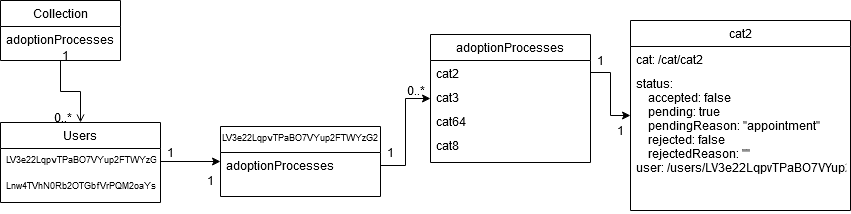
\includegraphics[width=\textwidth]{Images/adoptionProcesses file relations.png}
    \caption{Adoption Processes collection structure}
    \label{fig:adoptionProcessFileStructure}
\end{figure}

    
    \subsubsection{Cats Collection} \label{CATSCOLLECTION}
    The documents in the cat's collection are named after the Cat ID by concatenating the word cat with the id. This is to avoid it just being numbers and being harder to read. The contents of the documents are all of the information the application requires for the cat information displays, and all information is displayed in the app that is stored in these documents. An example of the file structure is given in the form of a UML class diagram representing the JSON files in Figure \ref{fig:catsCollectionFileStructure}
    
\begin{figure} [htbp!]
    \centering
    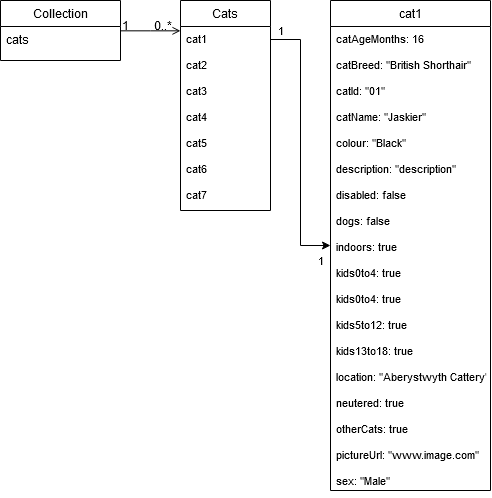
\includegraphics[width=\textwidth]{Images/CatsCollectionFileStructure.png}
    \caption{Cats Collection File Structure}
    \label{fig:catsCollectionFileStructure}
\end{figure}
    
    \subsubsection{Feedback Collection}
    The feedback collection is a collection of the feedback given by users from the app. The feedback documents are small; they contain the date, developerReplyRequested, the feedback, and a reference to the user's document. The feedback document names are a concatenation of their user Ids and the date-time. An example of feedback collection JSON structure is shown in Figure \ref{fig:feedbackCollectionFileStructure} as a UML Class diagram.
    
 \begin{figure} [htbp!]
    \centering
    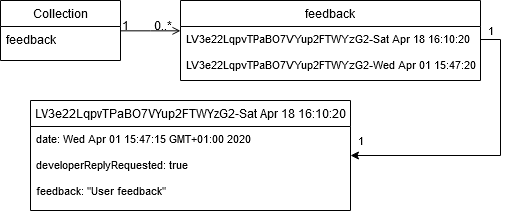
\includegraphics[width=\textwidth]{Images/FeedbackCollectionFileStructure.png}
    \caption{Feedback collection file structure}
    \label{fig:feedbackCollectionFileStructure}
\end{figure}  
    
    \subsubsection{Users Collection} \label{USERSCOLLECTION}
    The user's collection is the collection of user data, and each document has the name of the user's ID; the user ID is gained from the Firebase Authentication implementation (Section \ref{FIREBASEAUTHENTICATION}). The user documents contain the user's address, county, favouritedCats, mobileNumber, name, and postCode. An example of the users collection JSON file structure is found in Figure \ref{fig:usersCollectionFileStructure} as a UML Class diagram.
    
 \begin{figure} [htbp!]
    \centering
    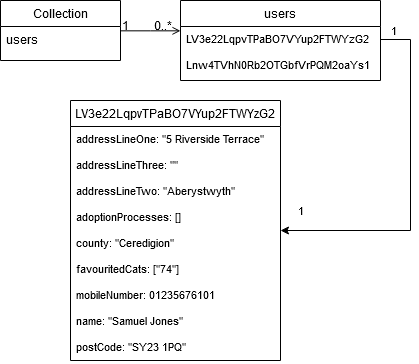
\includegraphics{Images/UserCollectionFileStructure.png}
    \caption{Users collection file structure}
    \label{fig:usersCollectionFileStructure}
\end{figure}   
    
    \subsection{Security Rules}
    The rules have been implemented in a way that restricts access to the database, for everything to some degree. A user must provide an authenticated user id for read or write operations in the user's collection. It is not possible to write to the cat collection, but anyone using a correctly connected application can read cat data. adoptionProcesses data can only be written or read by a correctly authenticated user liked user data. Feedback is unreadable by applications but writable by technically any authenticated application, but the app requires a login.
    
    When a collection is un-readable, or un-writeable by an application connected to the Firestore, this does not include the Firebase console, which allows administrator access to change any values, and read anything.
    
    Security rules for Firebase are easy to update and propagate within 5 minutes across all of the Firebase servers. It provides heavy adaptability at a moments notice so temporary changes could be done if needed like when the Server Scripts are run.
    
    The security rules in use by the Firestore are as follows:
    
\begin{verbatim}
rules_version = '2';
service cloud.firestore {
    match /databases/{database}/documents {
    match /users/{userId} {
        allow read, write: if request.auth.uid == userId
    }
    match /cats/{documents=*}{
        allow read: if true;
        allow write: if false;
    }
    match /adoptionProcesses/{userId}/adoptionProcesses/
                                    {documents=**}{
        allow read, write: if request.auth.uid == userId
    }
    match /feedback/{documents=**}{
        allow write: if true
        allow read: if false
    }
  }
}    
\end{verbatim}

    
    \subsection{Server Scripts} \label{SERVERSCRIPTS}
    The Server Scripts were created when I need to generate a lot of data fast, and I used them with some made-up data in JSON files to create 90 new cat objects. The script for creation was made with the intention to be scale-able, for example, if there was a need for 1 or 1000 extra cats that could be done, the script might get repetitive due to the lack of extra data, but if extra data were added to the JSON files, then it would use it accordingly.
    
    The second script that was made to interact with the server is the remove a certain number of cats script. After the first version of my creates a cat script was created, I realised that 90 cats had been generated incorrectly. The script deletes the cats between 2 numbers input into it in this scenario 10 and 90 was required.
    
    Both scripts required API keys for the Firestore, and these are not available to the public as they are privately linked to my Firestore account. The code in Appendix Sections \ref{CREATECATSCRIPT} and \ref{REMOVECATSSCRIPT}.
    
    Both scripts also use the Cat Class (Appendix Section \ref{CATCLASSSCRIPT}). It makes sense to separate shared code between the scripts, to reduce code duplication, increase stability, and maintainability.

\section{Technologies Used}
This section will talk about how the technologies that have been chosen are implemented in this project. The technologies in question are, Firebase Authentication, Firebase Firestore, Firebase File Storage, Firebase UI Integration Tests, Picasso, Kotlin, Material Design, Android X
    \subsection{Firebase}
    Google Firebase is a set of tools for application developers to integrate into their applications, that are easy to plug in and can quickly implement significant functionality with little effort. While, some features of Firebase make a lot of sense to be implemented on an application going to an audience, since this application is not destined for that path I did not add them, these features include Analytics and Cloud Messaging. This subsection talks about the libraries from Google Firebase that were used and go into detail about their implementation.
        \subsubsection{Authentication and Authentication UI} \label{FIREBASEAUTHENTICATION}
        Firebase Authentication is crucial to the functionality of the application; a large portion of the app is locked behind a login screen. Adoption, Feedback, My Account, and Cat Saving all require correct authentication for all or partial functionality. Authentication can be completed using many 3rd party authentication methods, including Google, Facebook, Twitter, Apple ID and more \cite{FIREBASEAUTHTYPES}. The application only allows for the use of google sign in, which is incredibly easy on Android and most users will have this, and an application-specific email and password. The mentality behind only using the two authentication methods is because it keeps things simple, it reduces chances for users to become confused as to what they signed in with, and it was the two easiest methods to implement.
        
        Firebase Authentication has a support library called Firebase Authentication UI which allows an application to drop in an activity which handles authentication. To do this you "build" the methods that you want to use and pass it to the Activity, when the Activity returns it will return either success or not, with success you are logged in. Firebase Authentication UI is a very nice and easy to use implementation of a login screen, with minimal implementation requirement.
        
        Firebase Authentication UI launch code for Google and Email/password logins:
        \begin{verbatim}
// Choose authentication providers
val providers = arrayListOf(
    AuthUI.IdpConfig.EmailBuilder().build(),
    AuthUI.IdpConfig.GoogleBuilder().build()
)

// Create and launch sign-in intent
startActivityForResult(
    AuthUI.getInstance()
        .createSignInIntentBuilder()
        .setAvailableProviders(providers)
        .setIsSmartLockEnabled(false, true)
        .build(),
    RC_SIGN_IN
)
        \end{verbatim}
        
        It is possible to check the Activity results another way, by calling checking if \newline "FirebaseAuth.getInstance().currentUser" returns a FirebaseUser object, if so there was a successful login for this application, and it has yet to be logged out (This includes if you have just started the application and had previously been logged in), or null if a login has not been performed or the user logged out.

        \subsubsection{Firestore}
        Firebase Firestore is google's latest attempt at providing real-time database support for application development, and it replaced their earlier attempt called Realtime Database, it has simplified security rules and more straightforward implementation on the firebase console. Firestore represents a scalable database implementation in the form of a NoSQL file structure utilising JSON files. Firestore can be interacted with in many ways in multiple languages including, JavaScript, Swift, Objective-C, Java, Java Android, Kotlin Android, Python, C++, Node-JS, GO, PHP, Unity, C\#, and Ruby.
        
        Most of the Firestore configuration and implementation is discussed in section \ref{FIREBASECONFIGURATION}.
        
        \subsubsection{File Storage}
        Google Firebase Storage is a cheap, scalable, secure, and easy to use storage medium in the cloud. In the aspect of this project, it is used to provide storage for cat images. The cat images are easily accessible where anyone can read them from a given URL, these URLs are used in the Firestore (Section \ref{FIREBASECONFIGURATION}) cats collection. 
        
        The security rules are much more basic, this time it is true for all read, and false of all write on all paths in the storage, as it is only storing the cat pictures:
        
        \begin{verbatim}
rules_version = '2';
service firebase.storage {
  match /b/{bucket}/o {
    match /{allPaths=**} {
      allow read: if true;
      allow write: if false;
    }
  }
}
        \end{verbatim}
        
        \subsubsection{UI Integration Tests}
        Google Firebase offers UI Instrumentation tests, which have been used in this project as Integration tests. The project does not make direct use of the Firebase functionality but rather indirectly via Bitrise. The way these tests work is via compiling a test APK using the Android Instrumentation tests and sending it to Firebase to be run on a matrix of testing devices, and the APK can then be run on many types of devices and all Android API levels.
        
        \subsubsection{Firestore Recycler Adapter}
        The FirestoreRecyclerAdapter is used with the RecyclerAdapter, it works using a Firestore query. It will asynchronously populate the RecyclerView and bind the data retrieved by the query to the RecyclerView.ItemHolder. It has been used for all adoption statuses, cat finder tools, and saved cat scrollables. An example of the adapter being setup and given to a RecyclerView is as follows, the adapter needs a FirestoreRecyclerOptions object which first is constructed using the query:
        
\begin{verbatim}
val query = FirebaseFirestore.getInstance()
    .collection("adoptionProcesses")
    .document(DataService.INSTANCE.user!!.uid)
    .collection("adoptionProcesses")
    .limit(10)

val options = FirestoreRecyclerOptions
    .Builder<AdoptionProcess>()
    .setQuery(query, AdoptionProcess::class.java)
    .setLifecycleOwner(this)
    .build()

val adapter =
    object : FirestoreRecyclerAdapter<
    AdoptionProcess, AdoptionStatusCard>(options) {
        override fun onCreateViewHolder
            (parent: ViewGroup, viewType: Int): 
            AdoptionStatusCard {
            val localView = LayoutInflater.from(parent.context)
                .inflate(R.layout.adoption_status_card,
                        parent, 
                        false)
            return AdoptionStatusCard(localView)
        }

        override fun onBindViewHolder(
            holder: AdoptionStatusCard,
            position: Int,
            model: AdoptionProcess
        ) {
            holder.bind(model)
        }
    }
\end{verbatim}

        \subsubsection{Filter Functionality using Queries}
        A key part of the function of the application's cat finder fragment is the implementation of the Firestore query. You can use a Firestore query to filter only specific types of data. This was used to great effect for the cat finder filter functionality, and it boils down to checking if the user wants to filter certain aspects, it is also possible to sort the list in a specific way in reverse orders based on how a user wants. The filter and sort functionality are supported directly by the queries. The cat finder implementation for the query generation is available in Appendix Section \ref{FIRESTOREQUERYIMPLEMENTATION}.
        
        \subsubsection{Adding Packaged APK UID to Firestore}
        In the firebase console, you need to add the SHA Certificate fingerprint, that relates to the bundled APK so that it can send requests to Google Firebase, in order to achieved this, inside Android Studio, you need to run 
        \begin{verbatim}
keytool -exportcert -list -v -alias <your-key-name> /
-keystore <path-to-production-keystore>
        \end{verbatim}
        According to the Firebase Documentation \cite{CLIENTAUTH}, you must add the SHA-1 or SHA256 key that is printed to the terminal to your firebase project settings for the application to interact correctly, this includes the debug, and release versions of the application made on each computer used to compile it unless the key is transferred between each.
        
    \subsection{Picasso}
    Picasso is a Library for Android, to load pictures into an ImageView from a URL, for example over the internet or on the local file system. It is straightforward to use, one line: Picasso.get().load("www.imageUrl.com/image").into(imageView). Picasso asynchronously downloads and inserts the image into the URL, it will cache the images for some time, meaning loading is much faster next time. Every image in the application that is not a Material Design icon is loaded using Picasso. Picasso allows other features such as transformation, use of placeholders, and Debug indicators.
    \subsection{Kotlin}
    Kotlin is a development language that works interchangeably with Java on the Java Virtual Machine. Its main features involve providing concise and easier development in a Java environment. It is the sole language in use for Android development in this project. Kotlin changes the classes and adds subsets such as the Data Classes which are used in this application.
    
    Throughout development, I made heavy usage of the lack of requirement for strong typing for local variables and instance variables that can have their type discerned before compile time. Kotlin boasts heavy co-routine support, and I was unable to utilise this in my project, as most asynchronous parts of the project are handled by 3rd-party libraries, as there is no use to reinvent the wheel.
    
    There are a few features of Kotlin that became very valuable when producing easy and concise code, these are Safe Call and Elvis Call operators. These were used to great effect in the following code excerpt:
\begin{verbatim}
val user = document.toObject<User>()
name.setText(user?.name ?: this.user!!.displayName)
addressLineOne.setText(user?.addressLineOne ?: "")
addressLineTwo.setText(user?.addressLineTwo ?: "")
addressLineThree.setText(user?.addressLineThree ?: "")
postCode.setText(user?.postCode ?: "")
county.setText(user?.county ?: "")
phone.setText(user?.mobileNumber ?: this.user!!.phoneNumber)
\end{verbatim}
    
    \subsection{Material Design}
    While most of Material Design's point, is the guidelines, to assist with the implementation of these guidelines, many of the functionalities suggested have a respective implementation for Android. While some of the guidelines have no implementations, and this application utilises the Material Design implementation of the \gls{Bottom Navigation Bar}, \gls{Card}, \gls{Up Button}, Switches, Text fields, Button, and Navigation Drawer. Material design components are implemented throughout my application, and I believe that they all improve the functionality, look, and general feel of the application.
    \subsection{AndroidX and Jetpack}
        AndroidX is the successor to AndroidCompat as a library, and it aims to support modern features in legacy APIs. Even though features may be in the Android Standard now, that doesn't mean they were previously, and to support these features in earlier APIs we use AndroidX. AndroidX is used so commonly throughout this application that the list would be too long to put in, but some features include ConstraintLayouts, GridLayouts, and the NestedScrollViews.
        
        Android Jetpack is a suite of libraries and tools that are aimed at helping developers write quick and high development applications. Jetpack aims to improve the way developers implement best practices. Android Jetpack is in the namespace of AndroidX; therefore, as a part of AndroidX, Jetpack is discussed as part of the same section.
        \subsubsection{NavigationUI} \label{NAVUI}
        NavigationUI is a relatively new methodology for navigation implementation inside of an Android Application. It utilises a Navigation Graph; the one used in the project is available in Appendix Section \ref{NAVIGATIONGRAPH}. The Navigation graph shows the hierarchy of the application; however since the navigation through this application is relatively simple, it requires only a flat hierarchy of navigation, with HomeFragment being the base of all navigation.
        
        NavigationUI offers the ability to add transition animations, and this application does not currently use them. The reason behind not using them is due to the lack of time, and the idea was to get navigation working before polishing the application later. NavigationUI also handles the animations and up to stack navigation in the app bar between Navigation Draw. NavigationUI is usable throughout the application by calling "findNavController().navigate(fragmentId)".
        
        When you navigate somewhere, it adds this destination to the navigation stack, and when the \gls{Up Button} is pressed then it navigates up the navigation stack to where you previously were in the program.
        
        \subsubsection{Legacy Support for UI Elements} \label{LEGACYUI}
        Grid Layout is a layout that provides an easy to use the grid, and it often is not clear that a grid is used because these items can easily. It's a feature of AndroidX and the current modern Android API, but older versions of the Android SDK do not work with the Grid Layout as it was not implemented, in the case of this application 21-23 did not support Grid Layout, so the AndroidX version was used instead.
        
        Constraint Layout is a performance-friendly easy to use layout for simple and slightly more advanced layouts. It utilises constraints to reduce time spent determining layout sizes dynamically by the CPU, each element or component is placed within relation to another element or the parent using constraints based on their current positions, working from the top of the file downwards, Constraint Layouts are used throughout the project for simple screens that can easily be made as a Constraint Layout, for example, the settings, home, and adoption info view fragment all use the Constraint Layout.

\section{Notable Bugs}
In this section, the notable bugs are discussed as they have significantly impacted development or extra time was needed to source the problem looking at older APIs or discovering the issues, especially with the continuous integration.

    \subsection{Gridlayout - AndroidX}
    As discussed in section \ref{LEGACYUI}, the Grid Layout is not supported in earlier versions of Android. Some functionality used in the My Account screen and user information update screens, are not available in Android 21, 22 or 23. This was evident from the Continuous Integration UI tests, but it was hard to discover precisely what the issue was as it was stating Grid Layout did not inflate as it couldn't be found correctly. The functionality required was the "layout\_columnWeight" and "layout\_rowWeight" which is not supported on these lower APIs.
    
    \subsection{writeBoolean and readBoolean pre API 29}
    Parcelable is an interface implementation that allows a developer to implement it, and it is used quite extensively by the Data Classes in the application (Appendix Section \ref{DATACLASSEXAMPLE}). The data classes required these to be passed between fragments using the NavigationUI navigate methods (Section \ref{NAVUI}). Early on these methods were implemented using a rather new feature writeBoolean and readBoolean, in the UI Integration tests that were running every single device one test ran on, failed except API 29, this was because these two methods had not been implemented until very recently and were not available in a legacy package, so some alternate implementation had to be used.
    
    The alternate implementation was translating a Boolean into a String and back. These are my implementations to facilitate this:

\begin{verbatim}
fun boolToString(bool: Boolean) : String{
    return if (bool) "true" else "false"
}


fun stringToBool(string: String) : Boolean {
    // If not true then assumed false
    return string == "true"
}   
\end{verbatim}
    
    \subsection{Large Image Files Over the Internet}
    
    When the Cat \gls{Card}s were first added to the cat finder tool, it was noticed there was extreme lag, I was concerned this could have been caused by the database being slow or the FirebaseRecyclerAdapter having inefficiencies. However, it ended up being caused by the loading of images; this was because these images were rather large in resolution but being crammed into small ImageViews and processing and download times were causing stuttering and lag. The fix for this was to format and compress the images from their current state without diminishing their quality. I utilised a program called jpegoptim \cite{JPEGOPTIM}, to perform compression, optimisations, and resizing to drop the size of the image from multiple megabytes to below 50 kilobytes, yet still keeping a good enough quality for display on mobile phones.
    
    \subsection{Infinitely Adding to the Navigation Stack in Settings}
    When navigating to the settings screen it was possible to navigate to that screen infinitely from inside of the settings screen, this means that you could in theory infinitely navigate to the settings screen increasing the size of the navigation stack. Whilst not strictly a major problem, it did make it hard to use the \gls{Up Button} to navigate up the navigation stack. The settings navigation button was added to the application's app bar, which means that it is present on every screen, it is possible to remove but required more work to fix correctly than was left in the project. The way this was fixed was by disallowing navigation to the settings destination if already at the settings destination. This code is given in the example:
    
\begin{verbatim}
when (item.itemId) {
    R.id.actionSettingsButton -> {
        if (navController.currentDestination?.id 
                != R.id.settingsFragment){
            navController.navigate(R.id.settingsFragment)
            true
        }
        else
            super.onOptionsItemSelected(item)
    }
    else -> {
        super.onOptionsItemSelected(item)
    }
}
\end{verbatim}

\chapter{Quality Assurance}
This chapter will cover the overall effort of the project to ensure a quality result. This involved automated testing, manual testing, and utilising adequate coding standards to ensure good maintainability.

\section{Overall Approach to Testing}
The overall approach with testing should revolve around ensuring all main features are tested, it is understood that some features are less testable than others, but a best effort attempt must be made to this effect. Most of the program should be tested, so that when a developer changes something or uses something that is not available in earlier APIs it shows up during testing, this was invaluable whilst attempting to ensure that the application works between the all versions of Android it is aimed at, 21+.

\section{Automated Testing}

Ensuring that any change to your code base, that causes a regression in application functionality is sometimes crucial in tracking down exactly what code causes the error, as a stack trace may not be enough. To achieve automated testing it is possible to cause Android Studio to test a target which includes Instrumentation, and Unit tests, whenever a code change is made, this disadvantageous on anything but the most basic project because it will not only take a long time up to 10 minutes per change, but also slow your computer down. 

Bitrise is the solution, it is a cloud based free to open source projects platform specialised in phone development and testing for Android and iOS. It is discussed in detail earlier in the report in Section \ref{CI}. What was looked for in a Continuous Integration solution, was an easy to use, expandable and ability to test not only unit tests, but UI Integration tests on every single API, and language the application supports. Bitrise fits all of the requirements for a Continuous Integration platform set forth in this section, as long as the project is open-source, which it is.

The Automated tests are completed on Bitrise and for the repository can be shown with a green tick as all tests are passing that are conducted automatically, shown in Figure \ref{fig:bitriseBuilds}.

 \begin{figure} [htbp!]
        \centering
        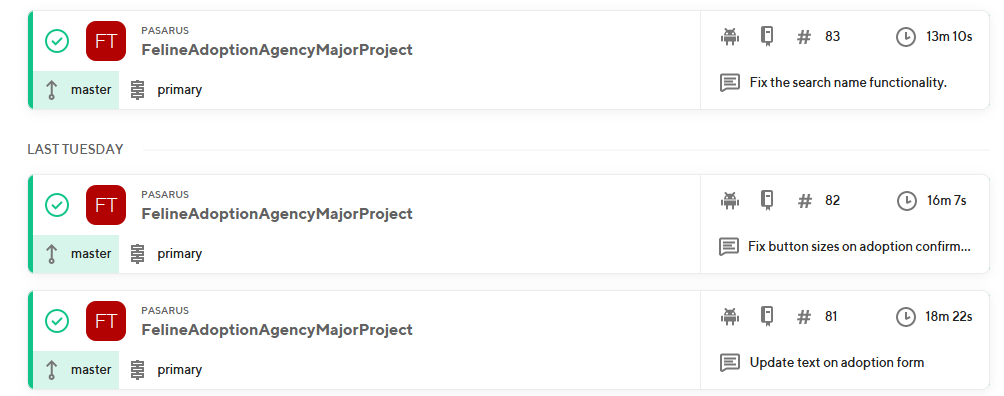
\includegraphics[width=\textwidth]{Images/Bitrise Repo Builds.PNG}
        \caption{The 3 most recent builds of the repository on Bitrise}
        \label{fig:bitriseBuilds}
    \end{figure}

\section{Test Implementations}

This project had a heavy emphasis on testing, where possible tests were implemented quickly and effectively. In some areas of the code base there is no testing, this revolves around the requirement for a user to log in, the main aim, was to provide testing not only on the Continuous Integration platform but locally, getting a Firebase Authenticated User and local Firebase database seemed challenging and thus was pushed to a later sprint, for when development of key user features had been completed, this was not possible given time constraints. Currently there is a lack of testing on any feature revolving around a user logging in, so manual testing must step in to fill this void.

The project implements 3 main areas of testing, manual testing, unit tests and user interface integration testing, the latter 2 of which is performed on every iteration of the code base that is committed to the GitHub repository.

    \subsection{Unit Tests}
    Unit Tests are currently in use for 2 files 1 class and 1 utilities file, this is because these are the parts of the system that can be tested without UI elements present. Meaning that the functionality and operation does not partially or completely require a Android Activity to be present in order to operate functionally. If a class or function is implemented separately from a Fragment or Activity. Every aspect of the classes and functions that are implemented should be tested to ensure guaranteed functionality, therefore every branch of code execution should be tested during testing with Unit Tests, this should be very possible and the test example shows this in Appendix Section \ref{Unit Test Example}. The Unit tests are ran on both Debug and Release testing sets during Continuous Integration builds, the completed tests on Bitrise are shown in Figure \ref{fig:UnitTestsStatus}.
    
    \begin{figure} [htbp!]
        \centering
        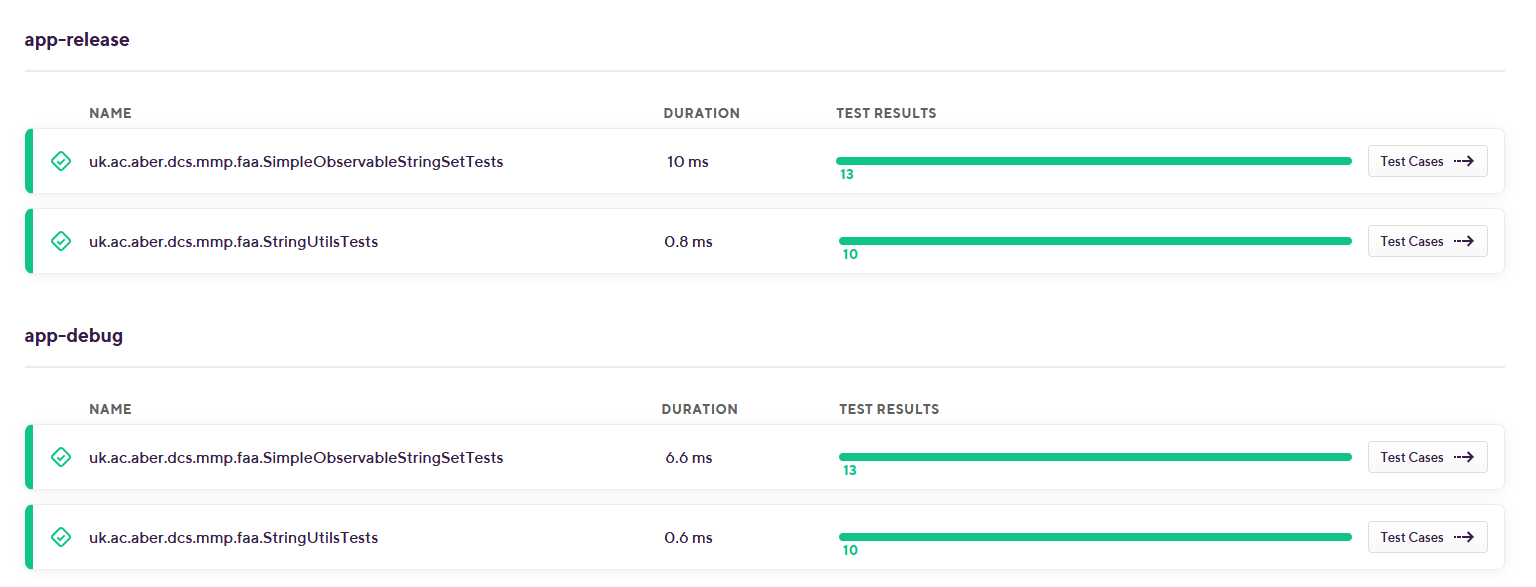
\includegraphics[width=\textwidth]{Images/UnitTestsBitrise.PNG}
        \caption{Unit Tests completion on most recent Bitrise Build}
        \label{fig:UnitTestsStatus}
    \end{figure}
    
    \subsection{User Interface Integration Testing}
    The project makes heavy use of UI Instrumentation tests in the form of Integration tests. Currently the project tests every UI aspect, to test that it is appearing correctly, with the exception of anything locked behind the Authentication methodology. The integration tests have the added benefit that they ensure that the application opens and all the tests can be ran on every API 21 and above, specifically via the usage of the Continuous Integration platform. The completed Bitrise UI Instrumentation Integration tests are shown to be completed in the Figure \ref{fig:UIIntegrationTests}.
    
    \begin{figure} [htbp!]
        \centering
        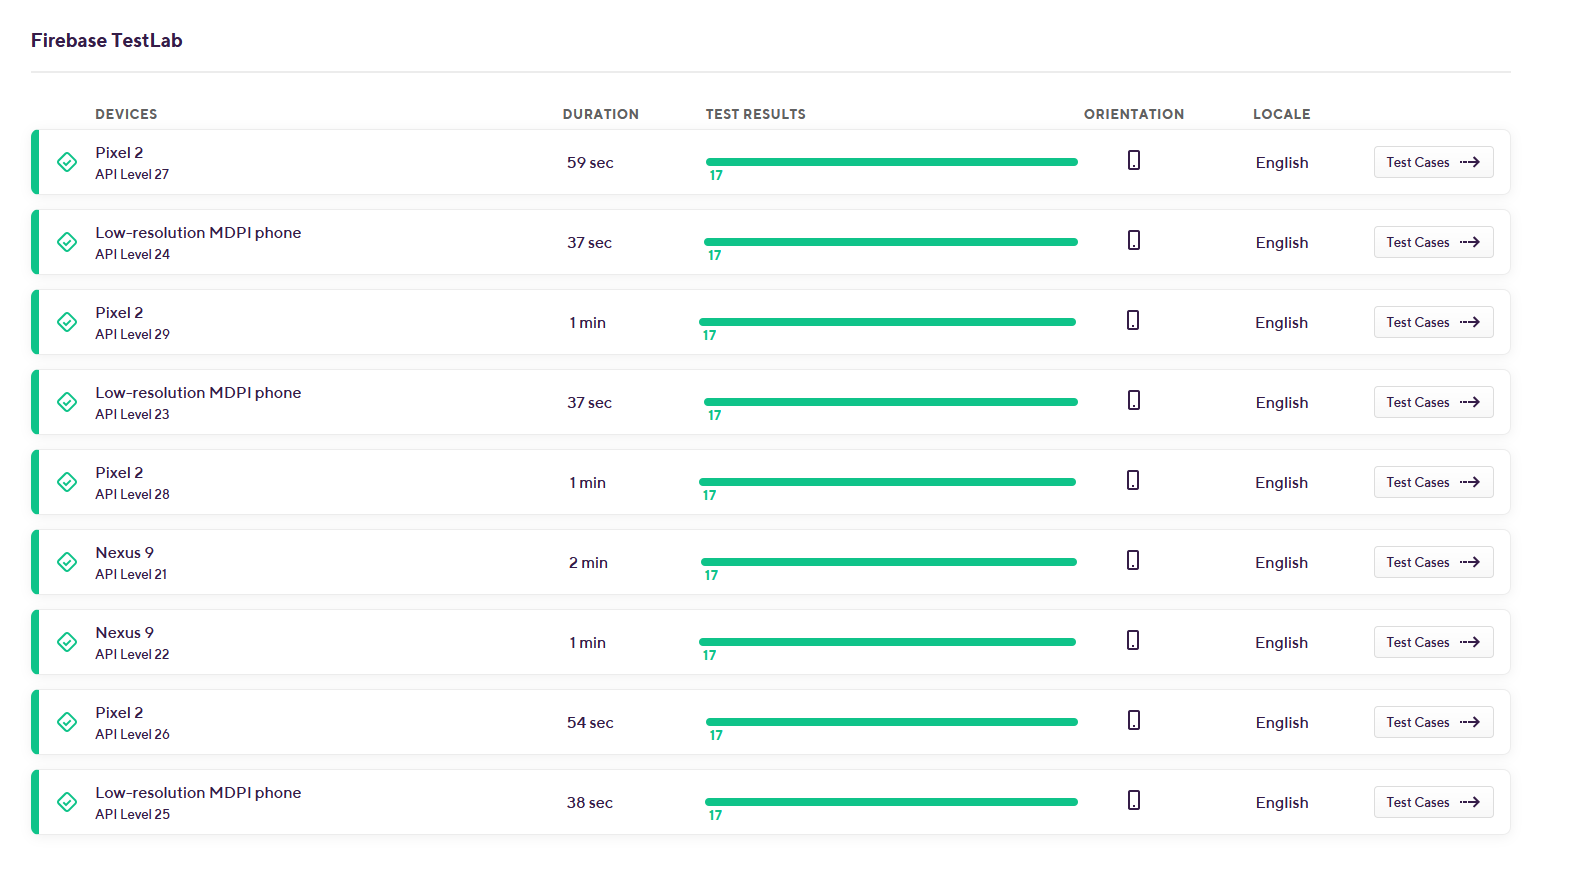
\includegraphics[width=\textwidth]{Images/UI Integration Tests Bitrise.PNG}
        \caption{UI Instrumentation Integration tests completion on most recent Bitrise Build}
        \label{fig:UIIntegrationTests}
    \end{figure}
    
    Each test is intended to be created using the Espresso test recorder, tested locally, ensuring that database connections are waited for correctly, and then pushed to the GitHub Repository, and monitored, if the tests fail a fix should be created and tested in the cycle again. These tests were absolutely instrumental in the development of the application as it lead to the discovery and fix of many high level UI and Application wide bugs, this echos the benefits of the tests.
    \clearpage

    \subsection{Manual Testing}
    Due to the lack of coverage of the Authentication features. The nature of manual testing ensures that the tester looks at most of the application and tries to find areas that have not worked well or are currently not fully functional. A Manual Testing table has been created to ensure that certain features are functional/present it is view-able on table \ref{tab:MANUALTESTINGSERVER}.

\footnotesize \small
\begin{longtable}{|l|l|l|l|l|}
\hline
\textbf{} &
  \textbf{Test Case Description} &
  \textbf{Test Steps} &
  \textbf{Expected Result} &
  \textbf{Pass/Fail} \\ \hline
\endhead
%
\#1 &
  \begin{tabular}[c]{@{}l@{}}Ensure login functionality\\  works\end{tabular} &
  \begin{tabular}[c]{@{}l@{}}1) Open application\\ 2) Tap navigation draw \\ button\\ 3) Tap login\\ 4) Select email\\ 5) Enter email\\ 6) Enter password\end{tabular} &
  \begin{tabular}[c]{@{}l@{}}1) User successfully logged in\\ 2) Adoption statuses should be \\ updated\\ 3) Nav draw login button\\  replaced with My Account \\ button\\ 4) Saved cats are shown on the\\  Saved Cats tab\end{tabular} &
  Pass \\ \hline
\#2 &
  \begin{tabular}[c]{@{}l@{}}Ensure Feedback \\ functionality works\end{tabular} &
  \begin{tabular}[c]{@{}l@{}}1) Login using test case \#1\\ 2) Tap nav draw\\ 3) Tap feedback\\ 4) Enter Feedback details \\ into feedback text box\\ 5) Tick the box to ask \\ to be replied to by the \\ developer\\ 6) Tap Send\end{tabular} &
  \begin{tabular}[c]{@{}l@{}}1) Feedback appears in the \\ Firebase Firestore feedback\\ collection under the logged in\\ User's UID and date.\end{tabular} &
  Pass \\ \hline
\#3 &
  \begin{tabular}[c]{@{}l@{}}Ensure user data is \\ synced across devices\end{tabular} &
  \begin{tabular}[c]{@{}l@{}}1) Login using test case \#1\\ 2) Tap nav draw\\ 3) Tap My Account\\ 4) Add or change the text\\  fields under the adoption\\  status and tap update.\\ 5) Tap logout\\ 6) Login again using \\ test case \#1\\ 7) Tap Nav Draw\\ 8) Tap My Account\end{tabular} &
  \begin{tabular}[c]{@{}l@{}}1) All changed or added text\\ should be loaded back into the\\ text fields.\end{tabular} &
  Pass \\ \hline
\#4 &
  \begin{tabular}[c]{@{}l@{}}Ensure saving cats\\  syncs across login\\  sessions and devices\end{tabular} &
  \begin{tabular}[c]{@{}l@{}}1) Login using test case \#1\\ 2) Tap the cat finder \\ button on Bottom \\ Navigation Bar\\ 3) Tap the heart icon on \\ a few Cat Cards\\ 4) Tap nav draw\\ 5) Tap My Account\\ 6) Tap Logout at the \\ bottom of the scroll\\ 7) Login again using\\  test case \#1\\ 8) Tap the saved cat \\ button on\end{tabular} &
  \begin{tabular}[c]{@{}l@{}}1) The cats that were saved\\  should appear on the screen\end{tabular} &
  Pass \\ \hline
\#5 &
  Adoption is functional &
  \begin{tabular}[c]{@{}l@{}}1) Login using test case \#1\\ 2) Tap the cat finder\\ button on Bottom\\ Navigation Bar\\ 3) Select a Cat Card\\ 4) Scroll to bottom\\ 5) Click Adopt This Cat!\\ 6) Fill/change data and tap \\ update\\ 7) Tap Yes\end{tabular} &
  \begin{tabular}[c]{@{}l@{}}1) Ensure that cat has appeared\\ in the adoption statuses\\ 2) Navigate to My Account and\\ ensure that the updated data is\\ present\end{tabular} &
  Pass \\ \hline
\#6 &
  Dark Mode is functional &
  \begin{tabular}[c]{@{}l@{}}1) Tap settings icon\\ 2) Flip Dark Mode switch\\ to on\\ 3) Tap the Up Button\\ 4) Tap the featured cat\\ 5) Tap the Up Button\\ 6) Tap each button on the\\ Bottom Navigation Bar\\ 7) Tap nav draw\\ 8) Navigate to each nav \\ draw location and then \\ back up to home before\\ continuing to the next\\ location, including\\ Settings, About, Login,\\ Help, and Feedback.\\ 9) Login using test case \#1\\ 10) Tap nav draw\\ 11) Tap My Account\\ 12) Tap an adoption status\\ card if present otherwise,\\ adopt a cat then come \\ back.\end{tabular} &
  \begin{tabular}[c]{@{}l@{}}1) Each of the screens should\\ look like the dark mode theme\\ is being used.\end{tabular} &
  Pass \\ \hline
\caption{Manual Testing table}
\label{tab:MANUALTESTINGSERVER}\\
\end{longtable}

\footnotesize \normalsize

\section{Coding Standards and Maintenance}

Using good coding standards makes code more readable and easier to maintain. For example, if a file contains multiple ways of defining a variable it can become harder to read and rather distracting. Enforcing a good use of comments and public API documentation allows a developer to understand how a class functions without ever looking at the code in the first place, this allows for quicker and easier maintenance and future development.

The Coding Standards in place on this project for Kotlin are provided on the Kotlin website \cite{KOTLINCODINGSTANDARDS}. It's a set of guidelines and helpful tips for easier to read Kotlin, if every developer on the team follows these standards it allows developers to read the code much faster and get less distracted.

Python also is used in the project specifically in the server scripts (Section \ref{SERVERSCRIPTS}) for Python the universal developer standards rest up on using the PEP8 standards \cite{PEP8STANDARDS}. The PEP8 standards are enforced by PyCharm, the IDE used during this project for Python development. 


\chapter{Evaluation}

This evaluation chapter attempts to evaluate the progress made, how time was spent and whether or not the project was successful in completing all of the stories. This chapter discusses the good things in the work and the aspects for which it can be improved. This evaluation should also cover how complete the application is and how the requirements fit into the end product.

\section{Requirements Completion}
This section focuses on discussing how complete each story is from Section \ref{STORIES}. The stories are listed with the completion level detailed beneath each story in a sub-list.

\begin{itemize}
    \item Design a working prototype of the application
    \begin{itemize}
        \item The application has a mostly functional prototype that gives any user the ability to understand how the application should function.
    \end{itemize}
    
    \item Refine the design of the prototype to ensure compliance with Material Design guidelines \cite{MATERIALDESIGNGUIDELINES}.
    \begin{itemize}
        \item The design was constantly refined throughout the production of the application, as discussed in Chapter \ref{IMPLEMENTATION}. The explicit design decisions that were changed were discussed in detail earlier in Section \ref{DESIGNCHANGESSECTION}, but Material Design was a heavy influence throughout the project.
    \end{itemize}
    
    \item Utilise a functional Continuous Integration software (Bitrise \cite{BITRISE}) to perform routine tests and ensure the application works across multiple devices, resolutions, and API versions.
    \begin{itemize}
        \item Bitrise was used continuously throughout the development cycle and will continue to work outside of this project. It tests devices on each API between 21 and 29, not only those but also most of the APIs use different screen sizes to ensure that parts are functional on both flagship smartphones and cheaper alternatives.
    \end{itemize}
    
    \item Stick to the multiple coding standards for Python (PEP8), Kotlin (Coding Style Guidelines) and any other languages that have been chosen on the GitHub Wiki
    \url{https://github.com/Pasarus/FelineAdoptionAgencyMajorProject/wiki}
    \begin{itemize}
        \item I stuck to the PEP8 standards for all python. The Kotlin style guideline was not always stuck to as I was new to the language and the style at the start of the project, but I believe that I have stuck as close as possible with my current level of expertise in Kotlin.
    \end{itemize}
    
    \item Create a Cat Finder tool in the application that allows a person to find a cat to adopt similar to Cats Protection's find-a-cat \cite{CATSPROTECTION}. This should be a list, probably a RecyclerView that has a Material\gls{Card} that allows us to view some basic details and save the cat. The Card should include Image, Name, Age, and Location with more details available on tap, opening a more information screen. This should be done in line with the Material Guidelines \cite{MATERIALDESIGNGUIDELINES}.
    \begin{itemize}
        \item The Cat Finder tool was fully implemented using, a RecyclerView and emulates most of the features from Cats Protection's find-a-cat. The \gls{Card} is functional and shows the Image, Name, Age, and Location of the cats, with further information available after tapping the cards, completed in line with Material Design Guidelines in all aspects except for Navigation Transitions functioning correctly.
    \end{itemize}
    
    \item A tool that displays detailed \gls{Card}s that represent the data of any Cat that has been saved by a user. These \gls{Card}s should be more detailed than those created in the Cat Finder tool, as these Cats are ones of keen interest to potential Adopters and should be featured as such.
    \begin{itemize}
        \item The Cat Saver functionality is fully implemented, and the saved Cats are synced by the user being logged in. The \gls{Card}s are more detailed than those in the Cat Finder tool and should keep users more interested in these cats.
    \end{itemize}
    
    \item Login functionality that allows a user to sync data across devices (their saved cats and user data), allow a user to adopt a cat only when logged in and view their status for approval of the adoption of a cat.
    \begin{itemize}
        \item Login functionality is fully implemented and is used to sync all data across multiple devices using one login account. It is implemented with Firebase Authentication.
    \end{itemize}
    
    \item Utilise Google Firebase as storage for all data required by the application, with appropriate security enforced to ensure that user data is protected in line with current EU and UK data protection legislation including GDPR \cite{GDPRARTICLE1}.
    \begin{itemize}
        \item The methodology of system security revolves around only storing data that is crucial to process function. All data is secure and transmitted using end-to-end encryption. Data is only available with a secure login to the Firebase Firestore at present.
    \end{itemize}
    
    \item Create adequate secondary screens to support the functionality of the application, including Settings, Help, Feedback, About, and My Account screens. When a user has logged in allow access to My Account otherwise request login before access is given because then data retrieval is possible.
    \begin{itemize}
        \item Settings is not fully implemented due to limitations from time; however, Help, Feedback, About and My Account screens are all fully functional.
    \end{itemize}
    
    \item Create a sufficiently well-presented Landing/Home screen that allows a user to see their adoption statuses, and a featured cat so users can immediately see a cat, and their adoption statuses as easily as possible. Keeping a user in the app if possible if they accidentally click on it, would potentially lead to more users adopting, the user is likely to be more distracted by the immediate availability of a cute featured cat.
    \begin{itemize}
        \item Home screen is created and feature complete. Featured cat functionality works well showing a random cat.
    \end{itemize}
    
    \item Support Android 21+ for development in an aim to make the application available to at minimum 85\% of all Android users.
    \begin{itemize}
        \item Android 21 to 29 is fully supported, and the application should work on all API variations in between. Confirmed via manual testing and continuous integration.
    \end{itemize}
    
    \item Provide a correctly signed and as functional as possible release version of the application as an APK for Android.
    \begin{itemize}
        \item APK has been signed correctly and constructed, tested on physical devices. Connection to Firebase is successful due to SHA1 certificate being present based on signed Android key.
    \end{itemize}
    
\end{itemize}

\section{Design Decisions}

Prototyping went very well, and it became invaluable during the implementation of the application. The prototype worked in the way that was hoped, and the prototype was used many times throughout the implementation sprints to guide design and influence decision making. 

UX Design overall has a few flaws. While the main screens and navigation methodologies are of good quality, the sub-screens, however, do have some features that overlap or should be redesigned to look and feel nicer to navigate and use. Notably, the adoption status information and cat information screens, while the prototype looks good the end-product does not have the same feel or easy on the eyes design, with more time I would like to improve those screens, as while they are functional, they are not pleasant to view.

DataService as a central function of the entire application was invaluable. It holds functionality needed throughout the application as well as holds key member variables that control the state of the application. To do this project again, I would heavily recommend the use of a Singleton class that holds an application state that is accessible without GUI components, that relates to the current application state. The DataService is used in almost all screens to some functionality, and without it, the application would not function, it, however, could, in theory, be replaced and allow the use of almost any other back-end.

Firebase is the fundamental backbone of the project. Firebase provides authentication functionality, data storage, file hosting, UI integration testing and secure communication with each feature. It's implementation while not necessarily easy, the tools have great interactability which would not necessarily have been possible without Firebase, given the time constraints.

The design process went overall quite well, and I believe that I followed the basic design principles I set out with. I found design was done in a waterfall fashion to a higher degree than my agile process would suggest, but that was due to the fact that Android applications require some UX prototyping before any other work can be completed.

\section{Tool Suitability}

GitHub is a git hosting platform with other tools for software development. It was used to great effect and became very useful, and its suitability is very high for this project. Use of the repository functionality including the wiki and Kanban project boards ensured the project could follow an agile approach, with the GitHub issues being prioritised on each sprint's project board.

Bitrise is a Continuous integration platform aimed at mobile application development. It has a very user-friendly interface, and integration took about 3 minutes to set up initially. While initial integration was not sufficient and had to be expanded upon, a great base test flow was given, to begin with.

Android Studio and PyCharm were the IDEs of choice when developing during this project. PyCharm was the IDE of choice for python development and worked flawlessly. Android Studio has a feature called AVM or Android Virtual Machine, and these AVMs do not run easily on AMD based processor architectures without some modifications, this is because of the way Intel has produced proprietary software for virtualisation of x86 architectures, while AMD lacks behind.

Coding Standards, the PEP8 and Kotlin Lang style guides are excellent standards for writing code that is maintainable and readable by a general developer who is just starting to get used to the language. It reduces jumbled code and allows a maintainer to jump in and produce the same level of code quality as the rest of the file.

Firebase was invaluable in the completion of the project and provided a solid, well tested, and free for low traffic backbone for development. Firebase is aimed towards the development of projects of this kind and was very suitable to the tasks it was used in.

With regards to testing, UI instrumentation tests where the UI tests are performed on many devices were invaluable, ensuring applications do start and navigation is performed correctly on all supported API levels. The unit testing is performed only on parts of the code base that does not require Activity, and as such is somewhat limited in scope, however, the testing coverage aim is an individual test class should test every branch of code execution in the class it is testing. The tools used for this were JUnit and espresso, espresso has a test recorder that made writing UI instrumentation tests much faster.

I found that by the end of the project, the tool suitability had been ironed out. I found that all of the tools that were used fit very well for their requirements in all stages of the project.

\section{How to Improve}

In this section, there is a discussion on how the project could have been improved if done again, including design decisions, time management, and code quality for both readability and maintainability.

    \subsection{Design Decisions}
    Ensuring broader research into tools available before designing and implementing what someone else has already done. Before I was made aware of Firebase and it's capabilities, I started to design and implement a web framework, that would, in essence, provide basic sign-in authentication, and data storage. I got far enough to have a basic RESTful API functional from my PC. Had I researched how it is done more thoroughly, I would have made the correct Design Decision earlier and saved myself work and time.
    
    \subsection{Time Management}
    As the project dragged, and as with a team size of 1, I found that sticking to a ridged agile process took too much time, if I were to start again, I would do away with the sprints and adopt a Kanban only approach. While a sprint gave ample opportunity for review, the time spent reviewing and rearranging the Kanban board every sprint could have been spent on development, design, and quality assurance.
    
    Notably, due to the COVID19 pandemic, my ability to focus and work on my dissertation was hampered by home life. With a younger brother, mother, and partner present at the house, I found my time for work dwindled rather rapidly. I would typically when writing a lengthy report, spend much time at the university planning and writing my report, this was not possible, but I would certainly do that if I were able to do it all over again.
    
    While my retrospectives and personal notes on how I progressed throughout the project are useful in writing this report, I firmly believe that the development of this project should have taken place at the same time as I was writing this report. The design chapter would have been easier to write shortly after the design was completed; the design is the part of the project completed earliest; the same is true for the other chapters.
    
    \subsection{Pull Requests and Code Review}
    If I were to start this project again, I would prefer to refine my workflow and replace the testing on every commit with the testing on pull requests and perform a code review of the produced code. While working in industry in a team, I found it invaluable to either look over my code again or have someone else with a fresh pair of eyes look at my code. Then when the builds have passed, I would merge the branch relating to the pull request, and this would reduce bugs and mean that the Master branch always had working code present according to the tests.
    
    \subsection{Automated Testing Login and Firebase Functionality}
    One major stickler for the maintainability for this application is the lack of testing for any login required features. While Manual tests were devised and should cover these areas, if these could be performed regularly on every commit with automated tests, and functional regression would be noticed immediately. 
    
    Furthermore testing that involved ensuring Database viability was more limited than it should be, while due to the nature of callback tests being hard to perform a better testing methodology should have been developed to improve detection of instability and feature regression further.
    
    With better test coverage, increased confidence could be had in utilising programming practices such as merciless refactoring, and more structured scrum sprints.
    
\section{Further Development}

To further development, there are a few things that would need to be worked on:

\begin{itemize}
    \item A UX design review, to ensure Material Design guidelines are followed
    \item Actual integration with real data for an adoption charity
    \item Refine of the filter features for the cat finder
    \item Improve how parts of the application look where there is no data to display such as default splash screens replace RecyclerViews
    \item Improve the Cat details screen and the Adoption status details screen
    \item Improve text scaling for different screen sizes
    \item Improve the form sections to ensure that all required details are given
    \item Location functionality instead of an actual address. Confirmed later as an address by an administrator.
    \item A separate application that is developed to ensure an administrator that can process applications and conduct appointments on time with the following features:
    \begin{itemize}
        \item Appointment request lists and the phone numbers to call
        \item Form to fill in appointment times
        \item Map integration to get to the address given using directions
        \item Checklist for investigations into the premises/user
        \item Ability to update the Cat list to ensure they are marked as reserved after an appointment has been confirmed.
        \item Tracking in case of emergency while on company/charity time, only while the app is in the foreground to avoid privacy invasion.
    \end{itemize}
\end{itemize}
% add any additional chapters here

% Setup glossary
\setemptyheader
\addcontentsline{toc}{chapter}{Glossary}
\printglossaries
\clearpage

%TC:ignore
\setemptyheader

\nocite{*} % include everything from the bibliography, irrespective of whether it has been referenced.

% the following line is included so that the bibliography is also shown in the table of contents. There is the possibility that this is added to the previous page for the bibliography. To address this, a newline is added so that it appears on the first page for the bibliography. 
\addcontentsline{toc}{chapter}{Annotated Bibliography} % Adds References to contents page

%
% example of including an annotated bibliography. The current style is an author date one. If you want to change, comment out the line and uncomment the subsequent line. You should also modify the packages included at the top (see the notes earlier in the file) and then trash your aux files and re-run. 
%\bibliographystyle{StylesAndReferences/authordate2annot}
\bibliographystyle{StylesAndReferences/IEEEannotU}
\renewcommand{\bibname}{Annotated Bibliography} 

\bibliography{StylesAndReferences/references} % References file


\setemptyheader

\addcontentsline{toc}{chapter}{Appendices}
\chapter*{Appendices}
The appendices are for additional content that is useful to support the discussion in the report. It is material that is not necessarily needed in the body of the report, but its inclusion in the appendices makes it easy to access. 

For example, if you have developed a Design Specification document as part of a plan-driven approach for the project, then it would be appropriate to include that document as an appendix. In the body of your report you would highlight the most interesting aspects of the design, referring your reader to the full specification for further detail.

If you have taken an agile approach to developing the project, then you may be less likely to have developed a full requirements specification. Perhaps you use stories to keep track of the functionality and the 'future conversations'. It might not be relevant to include all of those in the body of your report. Instead, you might include those in an appendix. 

There is a balance to be struck between what is relevant to include in the body of your report and whether additional supporting evidence is appropriate in the appendices. Speak to your supervisor or the module coordinator if you have questions about this.

\pagebreak

% start the appendix - sets up different numbering
\fancypagestyle{plain}{%
%\fancyhf{} % clear all header and footer fields
\fancyhead[L]{Appendix\ \thechapter}
\fancyhead[R]{\leftmark}}

\appendix
\fancyhead[L]{Appendix\ \thechapter}
\fancyhead[R]{\leftmark}
\fancyhead[C]{}
\fancyfoot[C]{\thepage}
\renewcommand{\headrulewidth}{0.4pt}
\renewcommand{\chaptermark}[1]{\markboth{#1}{}}

\fancyhead[L]{Appendix\ \thechapter}
\fancyhead[R]{\leftmark}
\fancyfoot[C]{{\thepage} of \pageref{LastPage}}

% include any appendices here
\chapter{Third-Party Code and Libraries}

% If you have made use of any third party code or software libraries, i.e. any code that you have not designed and written yourself, then you must include this appendix. 

% As has been said in lectures, it is acceptable and likely that you will make use of third-party code and software libraries. If third party code or libraries are used, your work will build on that to produce notable new work. The key requirement is that we understand what your original work is and what work is based on that of other people. 

% Therefore, you need to clearly state what you have used and where the original material can be found. Also, if you have made any changes to the original versions, you must explain what you have changed. 

% The following is an example of what you might say. 

% Apache POI library - The project has been used to read and write Microsoft Excel files (XLS) as part of the interaction with the client's existing system for processing data. Version 3.10-FINAL was used. The library is open source and it is available from the Apache Software Foundation 
% \cite{apache_poi}. The library is released using the Apache License 
% \cite{apache_license}. This library was used without modification. 

%Android SDK
Android SDK - The project used the SDK to compile the program for the Android Operating system, it was fundamentally crucial to the application's development and functionality to be included. Version 29.0.2 was used. The library and all documentation is provided under the Apache 2.0 License and was not modified.
\cite{APACHE2LICENSE}.

%Android X
Android X - Is a large library consisting on multiple smaller parts that are developed with the aim of improving backwards compatibility for modern Android application functionality. Android X was used for backwards compatible Navigation, layouts, testing, view model editing, and kotlin specific implementations. The following list describes all of the sub libraries used specifically which are also distributed open source under the Apache2.0 License and no libraries were modified. \cite{APACHE2LICENSE}
    \begin{itemize}
        \item androidx.appcompat:appcompat:1.1.0
        \item androidx.core:core-ktx:1.2.0
        \item androidx.constraintlayout:constraintlayout:1.1.3
        \item androidx.gridlayout:gridlayout:1.0.0
        \item androidx.navigation:navigation-ui-ktx:2.3.0-alpha04
        \item androidx.navigation:navigation-fragment-ktx:2.3.0-alpha04
        \item androidx.legacy:legacy-support-v4:1.0.0
        \item androidx.lifecycle:lifecycle-extensions:2.2.0
        \item androidx.lifecycle:lifecycle-viewmodel-ktx:2.2.0
        \item androidx.test.ext:junit:1.1.1
        \item androidx.test.espresso:espresso-core:3.2.0
        \item androidx.navigation:navigation-testing:2.3.0-alpha04
        \item androidx.test:rules:1.3.0-alpha05
    \end{itemize}


% Firebase
Firebase - is a set of libraries and source codes that are developed to work in tandem with the Google Firebase services for application development, they are fundamental to the core of the applications, Authentication, Notifications, Database, Image hosting, and some UI elements. These are provided as open source under a Apache 2.0 License and no library modifications were made. \cite{APACHE2LICENSE} The following list are specific libraries used.
    \begin{itemize}
        \item com.google.firebase:firebase-analytics:17.3.0
        \item com.google.firebase:firebase-auth:19.3.0
        \item com.firebaseui:firebase-ui-auth:6.2.0
        \item com.google.firebase:firebase-firestore-ktx:21.4.2
        \item com.firebaseui:firebase-ui-firestore:6.2.0
        \item com.google.firebase:firebase-database-ktx:19.2.1
        \item com.firebaseui:firebase-ui-database:6.2.0
        \item com.google.firebase:firebase-messaging:20.1.4
        \item com.google.gms.google-services
    \end{itemize}
    
% Picasso
Picasso - A library that is aimed at loading images from a url either online or offline and from the file store asynchronously into an Android Image View. These are provided under an Apache 2.0 License and no library modifications were made. \cite{APACHE2LICENSE} The version of the library used is 2.71828. 

% Material
Material Design - The library built to assist in the production of material design guided software, specifically used for the Material Design theme, \gls{Bottom Navigation Bar} and Material \gls{Card}. Open source and Provided under a Apache 2.0 license and was not modified \cite{APACHE2LICENSE}. Version used is 1.2.0-alpha05.

% Gradle
Gradle - The build system of choice when running Android Studio for development, it is crucial for building, testing and developing for the Android SDK. Open source and provided under an Apache 2.0 License and no library modifications were made \cite{APACHE2LICENSE}.

% Kotlin
Kotlin - Is the programming language of choice created by JetBrains as an alternative to a pure Java implementation, almost all of the project relies on Kotlin. Open source and provided under an Apache 2.0 license and no library modifications were made \cite{APACHE2LICENSE}. The Kotlin version in use is 1.3.71.
\chapter{Ethics Submission}

% This appendix includes a copy of the ethics submission for the project. After you have completed your Ethics submission, you will receive a PDF with a summary of the comments. That document should be embedded in this report, either as images, an embedded PDF or as copied text. The content should also include the Ethics Application Number that you receive. 

Assessment ID (reference): 15664

12/03/2020
For your information, please find below a copy of your
recently completed online ethics assessment

Next steps

Please refer to the email accompanying this attachment for details on the correct ethical
approval route for this project. You should also review the content below for any ethical
issues which have been flagged for your attention

Staff research - if you have completed this assessment for a grant application, you are not
required to obtain approval until you have received confirmation that the grant has been
awarded.

Please remember that collection must not commence until approval has been confirmed.

In case of any further queries, please visit www.aber.ac.uk/ethics or contact
ethics@aber.ac.uk quoting reference number 15664.

Assesment Details

AU Status
Undergraduate or PG Taught

Your aber.ac.uk email address
srj12@aber.ac.uk

Full Name
Samuel Robert Jones

Please enter the name of the person responsible for reviewing your assessment.
Reyer Zwiggelaar

Please enter the aber.ac.uk email address of the person responsible for reviewing
your assessment
rrz@aber.ac.uk

Supervisor or Institute Director of Research Department
cs

Module code (Only enter if you have been asked to do so)
CS39440

Proposed Study Title
Complete the Feline Adoption Agency App

Proposed Start Date
27 January 2020

Proposed Completion Date
01 June 2020

Are you conducting a quantitative or qualitative research project?
Mixed Methods

Does your research require external ethical approval under the Health Research
Authority?
No

Does your research involve animals?
Yes

Does your research involve human participants?
No

Are you completing this form for your own research?
Yes

Does your research involve human participants?
No

Institute
IMPACS

Please provide a brief summary of your project (150 word max)
CS31620 developed a prototype FAA app. This was left incomplete needing support for
many of the tabs. My task is to complete anything that was missing, and to improve any
areas as appropriate.

Where appropriate, do you have consent for the publication, reproduction or use of
any unpublished material?
Yes

Will appropriate measures be put in place for the secure and confidential storage of
data?
Yes

Does the research pose more than minimal and predictable risk to the researcher?
No

Will you be travelling, as a foreign national, in to any areas that the UK Foreign and
Commonwealth Office advise against travel to?
No

Please include any further relevant information for this section here:
If you are to be working alone with vulnerable people or children, you may need a
DBS (CRB) check. Tick to confirm that you will ensure you comply with this 
requirement should you identify that you require one.
Yes

Declaration: Please tick to confirm that you have completed this form to the best of
your knowledge and that you will inform your department should the proposal
significantly change.
Yes

Please include any further relevant information for this section here:
\chapter{Code Examples}

% For some projects, it might be relevant to include some code extracts in an appendix. You are not expected to put all of your code here - the correct place for all of your code is in the technical submission that is made in addition to the Project Report. However, if there are some notable aspects of the code that you discuss, including that in an appendix might be useful to make it easier for your readers to access. 

% As a general guide, if you are discussing short extracts of code then you are advised to include such code in the body of the report. If there is a longer extract that is relevant, then you might include it as shown in the following section. 

% Only include code in the appendix if that code is discussed and referred to in the body of the report. 

% \section{Random Number Generator}

% The Bayes Durham Shuffle ensures that the psuedo random numbers used in the simulation are further shuffled, ensuring minimal correlation between subsequent random outputs \cite{NumericalRecipes}.

% \begin{verbatim}
%  #define IM1 2147483563
%  #define IM2 2147483399
%  #define AM (1.0/IM1)
%  #define IMM1 (IM1-1)
%  #define IA1 40014
%  #define IA2 40692 
%  #define IQ1 53668
%  #define IQ2 52774
%  #define IR1 12211
%  #define IR2 3791
%  #define NTAB 32
%  #define NDIV (1+IMM1/NTAB)
%  #define EPS 1.2e-7
%  #define RNMX (1.0 - EPS)
 
%  double ran2(long *idum)
%  {
%   /*---------------------------------------------------*/
%   /* Minimum Standard Random Number Generator          */
%   /* Taken from Numerical recipies in C                */
%   /* Based on Park and Miller with Bays Durham Shuffle */
%   /* Coupled Schrage methods for extra periodicity     */
%   /* Always call with negative number to initialise    */
%   /*---------------------------------------------------*/	
 
%   int j;
%   long k;
%   static long idum2=123456789;
%   static long iy=0;
%   static long iv[NTAB];
%   double temp;
 
%   if (*idum <=0)
%   {
%      if (-(*idum) < 1)
%      {
%       *idum = 1;
%      }else
%      {
%       *idum = -(*idum);
%      }
%      idum2=(*idum);
%      for (j=NTAB+7;j>=0;j--)
%      {
%       k = (*idum)/IQ1;
%       *idum = IA1 *(*idum-k*IQ1) - IR1*k;
%       if (*idum < 0)
%       {
%          *idum += IM1;
%       }
%       if (j < NTAB)
%       {
%          iv[j] = *idum;
%       }
%      }
%      iy = iv[0];	
%   }
%   k = (*idum)/IQ1;
%   *idum = IA1*(*idum-k*IQ1) - IR1*k;
%   if (*idum < 0)
%   {
%      *idum += IM1;
%   }
%   k = (idum2)/IQ2;
%   idum2 = IA2*(idum2-k*IQ2) - IR2*k;
%   if (idum2 < 0)
%   {
%      idum2 += IM2;
%   }
%   j = iy/NDIV;
%   iy=iv[j] - idum2;
%   iv[j] = *idum;
%   if (iy < 1)
%   {
%      iy += IMM1;
%   }
%   if ((temp=AM*iy) > RNMX)
%   {
%      return RNMX;
%   }else
%   {
%      return temp;	
%   }
%  }
 
% \end{verbatim}

\section{Data Classes} \label {DATACLASSEXAMPLE}

\subsection{User}
\begin{verbatim}
data class User(
    var addressLineOne: String? = "",
    var addressLineTwo: String? = "",
    var addressLineThree: String? = "",
    var county: String? = "",
    var name: String? = "",
    var mobileNumber: String? = "",
    var postCode: String? = "",
    var favouritedCats: List<String>? = ArrayList(),
    var adoptionProcesses: List<DocumentReference>? = ArrayList()
)
\end{verbatim}
    
\subsection{Feedback}
\begin{verbatim}
class Feedback {

    var feedback: String? = null
    var developerReplyRequested: Boolean? = null
    var date: String? = null
    var userDocument: DocumentReference? = null

    constructor() {}
    constructor(
        feedback: String,
        devReplyRequested: Boolean,
        date: String,
        userDocument: DocumentReference
    ) {
        this.feedback = feedback
        this.developerReplyRequested = devReplyRequested
        this.date = date
        this.userDocument = userDocument
    }
}
\end{verbatim}

\subsection{Cat}
\begin{verbatim}
class Cat : Parcelable {

    var catAgeMonths: Int? = 0
    var catBreed: String? = ""
    var catName: String? = ""
    var colour: String? = ""
    var description: String? = ""
    var disabled: Boolean? = false
    var location: String? = ""
    var neutered: Boolean? = false
    var pictureUrl: String? = ""
    var dogs: Boolean? = false
    var indoors: Boolean? = false
    var kids0to4: Boolean? = false
    var kids13to18: Boolean? = false
    var kids5to12: Boolean? = false
    var otherCats: Boolean? = false
    var sex: String? = ""
    var catId: String? = ""

    constructor() : super()  // Needed for Firebase
    constructor(
        catAgeMonths: Int?,
        catBreed: String?,
        catName: String?,
        colour: String?,
        description: String?,
        disabled: Boolean?,
        location: String?,
        neutered: Boolean?,
        pictureUrl: String?,
        dogs: Boolean?,
        indoors: Boolean?,
        kids0to4: Boolean?,
        kids13to18: Boolean?,
        kids5to12: Boolean?,
        otherCats: Boolean?,
        sex: String?,
        catId: String?
    ) {
        this.catAgeMonths = catAgeMonths
        this.catBreed = catBreed
        this.catName = catName
        this.colour = colour
        this.description = description
        this.disabled = disabled
        this.location = location
        this.neutered = neutered
        this.pictureUrl = pictureUrl
        this.dogs = dogs
        this.indoors = indoors
        this.kids0to4 = kids0to4
        this.kids13to18 = kids13to18
        this.kids5to12 = kids5to12
        this.otherCats = otherCats
        this.sex = sex
        this.catId = catId
    }

    constructor(parcel: Parcel) : this() {
        catAgeMonths = parcel.readValue(Int::class.java.classLoader) as? Int
        catBreed = parcel.readString()
        catName = parcel.readString()
        colour = parcel.readString()
        description = parcel.readString()
        disabled = parcel.readValue(Boolean::class.java.classLoader) as? Boolean
        location = parcel.readString()
        neutered = parcel.readValue(Boolean::class.java.classLoader) as? Boolean
        pictureUrl = parcel.readString()
        sex = parcel.readString()
        catId = parcel.readString()
        dogs = stringToBool(parcel.readString() as String)
        indoors = stringToBool(parcel.readString() as String)
        kids0to4 = stringToBool(parcel.readString() as String)
        kids13to18 = stringToBool(parcel.readString() as String)
        kids5to12 = stringToBool(parcel.readString() as String)
        otherCats = stringToBool(parcel.readString() as String)
    }

    override fun writeToParcel(parcel: Parcel, flags: Int) {
        parcel.writeValue(catAgeMonths)
        parcel.writeString(catBreed)
        parcel.writeString(catName)
        parcel.writeString(colour)
        parcel.writeString(description)
        parcel.writeValue(disabled)
        parcel.writeString(location)
        parcel.writeValue(neutered)
        parcel.writeString(pictureUrl)
        parcel.writeString(sex)
        parcel.writeValue(catId)
        parcel.writeString(boolToString(dogs!!))
        parcel.writeString(boolToString(indoors!!))
        parcel.writeString(boolToString(kids0to4!!))
        parcel.writeString(boolToString(kids13to18!!))
        parcel.writeString(boolToString(kids5to12!!))
        parcel.writeString(boolToString(otherCats!!))
    }

    override fun describeContents(): Int {
        return 0
    }

    companion object CREATOR : Parcelable.Creator<Cat> {
        override fun createFromParcel(parcel: Parcel): Cat {
            return Cat(parcel)
        }

        override fun newArray(size: Int): Array<Cat?> {
            return arrayOfNulls(size)
        }
    }
}
\end{verbatim}

\subsection{AdoptionProcess}
\begin{verbatim}
class AdoptionProcess : Parcelable {
    var cat: DocumentReference? = null
    var status: MutableMap<String, Any>? = HashMap()
    var user: DocumentReference? = null

    constructor() : super()  // Needed for Firebase
    constructor(status: Map<String, Any>, cat: Cat) : this() {
        this.status = status.toMutableMap()
        this.cat = FirebaseFirestore.getInstance().collection("cats")
            .document("cat" + cat.catId)

        this.user = FirebaseFirestore.getInstance().collection("users").document(
            DataService.INSTANCE.user!!.uid
        )
    }

    constructor(parcel: Parcel) : this() {
        status!!["pending"] = stringToBool(parcel.readString() as String)
        status!!["pendingReason"] = parcel.readString() as String
        status!!["accepted"] = stringToBool(parcel.readString() as String)
        status!!["rejected"] = stringToBool(parcel.readString() as String)
        status!!["rejectedReason"] = parcel.readString() as String
        user = FirebaseFirestore.getInstance().document(parcel.readString() as String)
        cat = FirebaseFirestore.getInstance().document(parcel.readString() as String)
    }

    override fun writeToParcel(dest: Parcel?, flags: Int) {
        if (dest != null){
            val pending = status!!["pending"] as Boolean
            val pendingReason = status!!["pendingReason"] as String
            val accepted = status!!["accepted"] as Boolean
            val rejected = status!!["rejected"] as Boolean
            val rejectedReason = status!!["rejectedReason"] as String
            val user = this.user.toString()
            val cat = this.cat.toString()
            dest.writeString(boolToString(pending))
            dest.writeString(pendingReason)
            dest.writeString(boolToString(accepted))
            dest.writeString(boolToString(rejected))
            dest.writeString(rejectedReason)
            dest.writeString(user)
            dest.writeString(cat)
        }
    }

    override fun describeContents(): Int {
        return 0
    }

    companion object CREATOR : Parcelable.Creator<AdoptionProcess> {
        override fun createFromParcel(parcel: Parcel): AdoptionProcess {
            return AdoptionProcess(parcel)
        }

        override fun newArray(size: Int): Array<AdoptionProcess?> {
            return arrayOfNulls(size)
        }
    }
}
\end{verbatim}

\section{Server Scripts}

\subsection{Create Cats Script}\label{CREATECATSCRIPT}
\begin{verbatim}
import os
import firebase_admin
from google.cloud import firestore
from json import dump, load
from Cat import Cat
from random import randint


"""
This script was designed with the intention of generating cats for my MMP 
project continuing the Feline Adoption Agency App for Android. With that
in mind it utilizes a backend database from Google Firestore. For 
someone to use this script they must change 
GOOGLE_SERVICES_ACCOUNT_KEY_LOCATION to reflect their own database.
"""


GOOGLE_SERVICES_ACCOUNT_KEY_LOCATION = ""
FILE_PATH_TO_COPY_OF_CATS = "CatCopies/copy.json"
CAT_DETAILS_DIR = "CatDetails"
CAT_NAMES_FILE = "CatNames.json"
CAT_BREEDS_FILE = "CatBreeds.json"
CAT_DESCRIPTIONS_FILE = "CatDescriptions.json"
CAT_COLOURS_FILE = "CatColours.json"
CAT_LOCATIONS_FILE = "CatLocations.json"
CAT_PICTURES_URLS_FILE = "CatPictureUrls.json"
MAX_CAT_AGE_IN_MONTHS = 100
MIN_CAT_AGE_IN_MONTHS = 0
CAT_ID_TO_START_FROM = 10
CAT_ID_TO_END_AT = 100


def load_cat_breeds():
    with open(os.path.join(CAT_DETAILS_DIR, CAT_BREEDS_FILE)) as breeds_file:
        return load(breeds_file)


def load_cat_descriptions():
    with open(os.path.join(CAT_DETAILS_DIR, CAT_DESCRIPTIONS_FILE)) as \
    descriptions_file:
        return load(descriptions_file)


def load_cat_names():
    with open(os.path.join(CAT_DETAILS_DIR, CAT_NAMES_FILE)) as names_file:
        return load(names_file)


def load_colours():
    with open(os.path.join(CAT_DETAILS_DIR, CAT_COLOURS_FILE)) as colours_file:
        return load(colours_file)


def load_locations():
    with open(os.path.join(CAT_DETAILS_DIR, CAT_LOCATIONS_FILE)) as \
    locations_file:
        return load(locations_file)


def load_picture_urls():
    with open(os.path.join(CAT_DETAILS_DIR, CAT_PICTURES_URLS_FILE)) as \
    url_file:
        return load(url_file)


def load_cats_details():
    return load_cat_names(), load_cat_breeds(), \
    load_cat_descriptions(), load_colours(), \
    load_locations(), load_picture_urls()


def generate_cats():
    cats_list = []

    cat_names, cat_breeds, cat_descriptions, colours, locations, picture_urls \
    = load_cats_details()

    true_or_false = [True, False]
    male_or_female = [u"Male", u"Female"]

    for ii in range(CAT_ID_TO_START_FROM, CAT_ID_TO_END_AT):
        children = true_or_false[randint(0, 1)]
        cats_list.append(Cat(
            cat_name=cat_names[randint(0, len(cat_names) - 1)],
            cat_breed=cat_breeds[randint(0, len(cat_breeds) - 1)],
            description=cat_descriptions[randint(0,
                len(cat_descriptions) - 1)],
            cat_age_months=randint(
                a=MIN_CAT_AGE_IN_MONTHS,
                b=MAX_CAT_AGE_IN_MONTHS),
            cat_id=str(ii),
            colour=colours[randint(0, len(colours) - 1)],
            disabled=true_or_false[randint(0, 1)],
            neutered=true_or_false[randint(0, 1)],
            dogs=true_or_false[randint(0, 1)],
            indoors=true_or_false[randint(0, 1)],
            kids0to4=children,
            kids5to12=children,
            kids13to18=children,
            location=locations[randint(0, len(locations) - 1)],
            other_cats=true_or_false[randint(0, 1)],
            picture_url=picture_urls[randint(0, len(picture_urls) - 1)],
            sex=male_or_female[randint(0, 1)]
        ).to_dict())

    return cats_list


def upload_cats(cats_list):
    # Ensure that firestore is initialized:
    os.environ["GOOGLE_APPLICATION_CREDENTIALS"] = \ 
    GOOGLE_SERVICES_ACCOUNT_KEY_LOCATION
    firebase_admin.initialize_app()

    db = firestore.Client()

    for ii in range(CAT_ID_TO_START_FROM, CAT_ID_TO_END_AT):
        # Put each of the cats online in the correct file.
        db.collection("cats").document("cat"+str(ii)) \
        .set(cats_list[ii-CAT_ID_TO_START_FROM])


# This is the actual script that is ran, it subsequently calls 
# all the functions
cats = generate_cats()
with open(FILE_PATH_TO_COPY_OF_CATS, "w+") as file:
    dump(cats, file)
upload_cats(cats)
\end{verbatim}

\subsection{Remove Cats Script}\label{REMOVECATSSCRIPT}

\begin{verbatim}
"""
This script was made when I realised I made a mistake in my cat generation
script for all cat ids between 10 and 99. So this is designed at removing 
those cats. With that in mind it utilizes a backend database from Google Firestore.
For someone to use this script they must change
GOOGLE_SERVICES_ACCOUNT_KEY_LOCATION to reflect their own database.
"""
import os

import firebase_admin
from google.cloud import firestore

GOOGLE_SERVICES_ACCOUNT_KEY_LOCATION = ""
CAT_ID_TO_START_FROM = 10
CAT_ID_TO_END_AT = 100

os.environ["GOOGLE_APPLICATION_CREDENTIALS"] = \
GOOGLE_SERVICES_ACCOUNT_KEY_LOCATION
firebase_admin.initialize_app()

db = firestore.Client()

for ii in range(CAT_ID_TO_START_FROM, CAT_ID_TO_END_AT):
    db.collection("cats").document("cat" + str(ii)).delete()
\end{verbatim}

\subsection{Cat Class}\label{CATCLASSSCRIPT}
\begin{verbatim}
class Cat(object):
    def __init__(self, cat_age_months, cat_breed, cat_name, colour, 
                    description, disabled, location, neutered,
                    picture_url, dogs, indoors, kids0to4, kids13to18,
                    kids5to12, other_cats, sex, cat_id):
        self.cat_age_months = cat_age_months
        self.cat_breed = cat_breed
        self.cat_name = cat_name
        self.colour = colour
        self.description = description
        self.disabled = disabled
        self.location = location
        self.neutered = neutered
        self.picture_url = picture_url
        self.dogs = dogs
        self.indoors = indoors
        self.kids0to4 = kids0to4
        self.kids13to18 = kids13to18
        self.kids5to12 = kids5to12
        self.other_cats = other_cats
        self.sex = sex
        self.cat_id = cat_id

    def to_dict(self):
        return {
            u"catAgeMonths": self.cat_age_months,
            u"catBreed": self.cat_breed,
            u"catName": self.cat_name,
            u"colour": self.colour,
            u"description": self.description,
            u"disabled": self.disabled,
            u"location": self.location,
            u"neutered": self.neutered,
            u"pictureUrl": self.picture_url,
            u"dogs": self.dogs,
            u"indoors": self.indoors,
            u"kids0to4": self.kids0to4,
            u"kids13to18": self.kids13to18,
            u"kids5to12": self.kids5to12,
            u"otherCats": self.other_cats,
            u"sex": self.sex,
            u"catId": self.cat_id
        }
\end{verbatim}

\section{NavigationUI Navigation Graph} \label{NAVIGATIONGRAPH}
\begin{verbatim}
    <?xml version="1.0" encoding="utf-8"?>

<!-- Copyright 2020 Samuel Jones

   Licensed under the Apache License, Version 2.0 (the "License");
   you may not use this file except in compliance with the License.
   You may obtain a copy of the License at

       http://www.apache.org/licenses/LICENSE-2.0

   Unless required by applicable law or agreed to in writing, software
   distributed under the License is distributed on an "AS IS" BASIS,
   WITHOUT WARRANTIES OR CONDITIONS OF ANY KIND, either express or implied.
   See the License for the specific language governing permissions and
   limitations under the License. -->

<navigation xmlns:android="http://schemas.android.com/apk/res/android"
    xmlns:app="http://schemas.android.com/apk/res-auto"
    xmlns:tools="http://schemas.android.com/tools"
    android:id="@+id/nav_graph"
    app:startDestination="@id/homeFragment">

    <fragment
        android:id="@+id/settingsFragment"
        android:name="uk.ac.aber.dcs.mmp.faa.ui.settings.SettingsFragment"
        android:label="Settings"
        tools:layout="@layout/settings_fragment" />
    <fragment
        android:id="@+id/myAccountFragment"
        android:name="uk.ac.aber.dcs.mmp.faa.ui.account.MyAccountFragment"
        android:label="Account Details"
        tools:layout="@layout/my_account_fragment" />
    <fragment
        android:id="@+id/helpFragment"
        android:name="uk.ac.aber.dcs.mmp.faa.ui.help.HelpFragment"
        android:label="Help"
        tools:layout="@layout/help_fragment" />
    <fragment
        android:id="@+id/aboutFragment"
        android:name="uk.ac.aber.dcs.mmp.faa.ui.about.AboutFragment"
        android:label="About"
        tools:layout="@layout/about_fragment" />
    <fragment
        android:id="@+id/feedbackFragment"
        android:name="uk.ac.aber.dcs.mmp.faa.ui.feedback.FeedbackFragment"
        android:label="Feedback"
        tools:layout="@layout/feedback_fragment" />
    <fragment
        android:id="@+id/homeFragment"
        android:name="uk.ac.aber.dcs.mmp.faa.ui.home.HomeFragment"
        android:label="Home"
        tools:layout="@layout/home_fragment" >
        <action
            android:id="@+id/action_homeFragment_to_settingsFragment"
            app:destination="@id/settingsFragment" />
        <action
            android:id="@+id/action_homeFragment_to_myAccountFragment"
            app:destination="@id/myAccountFragment" />
        <action
            android:id="@+id/action_homeFragment_to_helpFragment"
            app:destination="@id/helpFragment" />
        <action
            android:id="@+id/action_homeFragment_to_aboutFragment"
            app:destination="@id/aboutFragment" />
        <action
            android:id="@+id/action_homeFragment_to_feedbackFragment"
            app:destination="@id/feedbackFragment" />
        <action
            android:id="@+id/action_homeFragment_to_savedFragment"
            app:destination="@id/savedFragment" />
        <action
            android:id="@+id/action_homeFragment_to_findCatFragment"
            app:destination="@id/findCatFragment" />
        <action
            android:id=
            "@+id/action_homeFragment_to_adoptionStatusInfoViewFragment"
            app:destination="@id/adoptionStatusInfoViewFragment" />
        <action
            android:id="@+id/action_homeFragment_to_catCardInfoFragment"
            app:destination="@id/catCardInfoFragment" />
        <action
            android:id="@+id/action_homeFragment_to_adoptionForm"
            app:destination="@id/adoptionForm" />
        <action
            android:id="@+id/action_homeFragment_to_adoptionFormConfirmation"
            app:destination="@id/adoptionFormConfirmation" />
        <action
            android:id="@+id/action_homeFragment_to_cancel_adoption_dialog"
            app:destination="@id/cancel_adoption_dialog" />
    </fragment>
    <fragment
        android:id="@+id/savedFragment"
        android:name="uk.ac.aber.dcs.mmp.faa.ui.saved.SavedFragment"
        android:label="Saved Cats"
        tools:layout="@layout/saved_fragment" />
    <fragment
        android:id="@+id/findCatFragment"
        android:name="uk.ac.aber.dcs.mmp.faa.ui.findcat.FindCatFragment"
        android:label="Find A Cat Tool"
        tools:layout="@layout/find_cat_fragment" />
    <fragment
        android:id="@+id/adoptionStatusInfoViewFragment"
    android:name="uk.ac.aber.dcs.mmp.faa.ui.adoption.
                                    AdoptionStatusInfoViewFragment"
        android:label="Adoption Status Info"
        tools:layout="@layout/adoption_status_info_view_fragment" />
    <fragment
        android:id="@+id/catCardInfoFragment"
        android:name="uk.ac.aber.dcs.mmp.faa.ui.catinfo.CatCardInfoFragment"
        android:label="More Info"
        tools:layout="@layout/cat_card_info_fragment" />
    <fragment
        android:id="@+id/adoptionForm"
        android:name="uk.ac.aber.dcs.mmp.faa.ui.adoption.AdoptionForm"
        android:label="Adoption Form"
        tools:layout="@layout/fragment_adoption_form" />
    <fragment
        android:id="@+id/adoptionFormConfirmation"
        android:name="uk.ac.aber.dcs.mmp.faa.ui.adoption.
                                AdoptionFormConfirmation"
        android:label="Adoption Confirmation"
        tools:layout="@layout/fragment_adoption_form_confirmation" />
    <dialog
        android:id="@+id/cancel_adoption_dialog"
        android:name="uk.ac.aber.dcs.mmp.faa.ui.adoption.CancelAdoptionDialog"
        android:label="Adoption Cancellation confirmation"
        tools:layout="@layout/fragment_cancel_adoption_dialog" />
</navigation>
\end{verbatim}

\section{Firebase Filter Implementation} \label{FIRESTOREQUERYIMPLEMENTATION}
\begin{verbatim}
var query: Query = FirebaseFirestore.getInstance().collection("cats")

val location = map["location"]
if (location != "") {
    query = query.whereEqualTo("location", location)
}

val families = map["families"]
if (families != "") {
    if (families == "Children") {
        query = query.whereEqualTo("kids0to4", true)
        query = query.whereEqualTo("kids5to12", true)
        query = query.whereEqualTo("kids13to18", true)
    } else if (families == "No Children") {
        query = query.whereEqualTo("kids0to4", false)
        query = query.whereEqualTo("kids5to12", false)
        query = query.whereEqualTo("kids13to18", false)
    }
}

val otherCats = map["otherCats"]
if (otherCats != "") {
    if (otherCats == "Other cats welcome") {
        query = query.whereEqualTo("otherCats", true)
    } else if (otherCats == "No other cats") {
        query = query.whereEqualTo("otherCats", false)
    }
}

val dogs = map["dogs"]
if (dogs != "") {
    if (dogs == "Happy with Dogs") {
        query = query.whereEqualTo("dogs", true)
    } else if (dogs == "Unhappy with Dogs") {
        query = query.whereEqualTo("dogs", false)
    }
}

val indoors = map["indoorsOnly"]
if (indoors != "") {
    if (indoors == "Indoors only") {
        query = query.whereEqualTo("indoors", true)
    } else if (indoors == "Needs outside access") {
        query = query.whereEqualTo("indoors", false)
    }
}

val sortBy = map["sortBy"]
var orderByString = ""
when (sortBy) {
    "Name" -> {
        orderByString = "catName"
    }
    "Age" -> {
        orderByString = "catAgeMonths"
    }
    "Recently Listed" -> {
        orderByString = "catId"
    }
}

query = if (map["sortByOrdering"] == "Ascending"){
    query.orderBy(orderByString, Query.Direction.ASCENDING)
} else {
    query.orderBy(orderByString, Query.Direction.DESCENDING)
}

val name = map["name"]
if (name != "") {
    query = query.startAt(name).endAt(name + "\uf8ff")
}
\end{verbatim}

\section{Testing Examples} 
The following are examples given for testing in the project.

\subsection{Unit Test example} \label{Unit Test Example}
\begin{verbatim}
import junit.framework.Assert.assertEquals
import org.junit.Before
import org.junit.Test
import uk.ac.aber.dcs.mmp.faa.utils.ObserverOfStringSet
import uk.ac.aber.dcs.mmp.faa.utils.SimpleObservableStringSet

class SimpleObservableStringSetTests : ObserverOfStringSet {
    private var addCalledCount: Int = 0
    private var removeCalledCount: Int = 0
    private lateinit var testSet: SimpleObservableStringSet

    @Before
    fun setUp() {
        addCalledCount = 0
        removeCalledCount = 0
        testSet = SimpleObservableStringSet()
        testSet.addObserver(this)
    }

    override fun onObservedAdd(e: String) {
        addCalledCount += 1
    }

    override fun onObservedRemove(e: String) {
        removeCalledCount += 1
    }

    @Test
    fun test_notifiesObserversOnAdd() {
        testSet.add("test1")
        assertEquals(addCalledCount, 1)
    }

    @Test
    fun test_notifiesObserversOnAddOfDuplicate() {
        val test1 = "test1"
        testSet.add(test1)
        assertEquals(addCalledCount, 1)
        testSet.add(test1)
        assertEquals(addCalledCount, 2)
    }

    @Test
    fun test_notifiesObserversOnRemove() {
        val test1 = "test1"
        testSet.add(test1)
        testSet.remove(test1)
        assertEquals(addCalledCount, 1)
        assertEquals(removeCalledCount, 1)
    }

    @Test
    fun test_notifiesObserversOnRemoveOfNoneExistentString() {
        testSet.remove("test1")
        assertEquals(removeCalledCount, 1)
    }

    @Test
    fun test_notifiesMultipleTimesForMultipleAdds() {
        testSet.add("test1")
        assertEquals(addCalledCount, 1)
        testSet.add("test2")
        assertEquals(addCalledCount, 2)
        testSet.add("test3")
        assertEquals(addCalledCount, 3)
    }

    @Test
    fun test_notifiesMultipleTimesForMultipleRemoves() {
        val test1 = "test1"
        val test2 = "test2"
        val test3 = "test3"
        testSet.add(test1)
        assertEquals(addCalledCount, 1)
        testSet.add(test2)
        assertEquals(addCalledCount, 2)
        testSet.add(test3)
        assertEquals(addCalledCount, 3)
        testSet.remove(test1)
        assertEquals(removeCalledCount, 1)
        testSet.remove(test2)
        assertEquals(removeCalledCount, 2)
        testSet.remove(test3)
        assertEquals(removeCalledCount, 3)
    }

    @Test
    fun test_notifiesOncePerItemAddedWhenAddingMultipleItemsWithAddAll() {
        testSet.addAll(setOf("test1", "test2", "test3"))
        assertEquals(addCalledCount, 3)
    }

    @Test
    fun test_notifiesOncePerItemClearedWhenUsingClear() {
        testSet.addAll(setOf("test1", "test2", "test3"))
        assertEquals(addCalledCount, 3)

        testSet.clear()
        assertEquals(removeCalledCount, 3)
    }

    @Test
    fun test_notifiesOncePerItemClearedWhenRemovingMultipleItemsWithRemoveAll() {
        testSet.addAll(setOf("test1", "test2", "test3"))
        assertEquals(addCalledCount, 3)

        testSet.removeAll(setOf("test1", "test2", "test3"))
        assertEquals(removeCalledCount, 3)
    }

    // Tests below this point are to ensure that basic set functionality
    // is still viable via this class
    @Test
    fun test_setSizeOption() {
        for (i in 1..10) {
            testSet.add("" + i)
            assertEquals(testSet.size, i)
        }
    }

    @Test
    fun test_setUniquenessIsGuarenteed() {
        val test1 = "test1"
        testSet.add(test1)
        assertEquals(testSet.size, 1)
        testSet.add(test1)
        assertEquals(testSet.size, 1)

        // Ensure the value in the set is test1
        for (wannabeTest1 in testSet) {
            assertEquals(wannabeTest1, test1)
        }
    }

    @Test
    fun test_setRetrievalViaIteratorStillWorks() {
        val test1 = "test1"
        testSet.add(test1)
        for (wannabeTest1 in testSet) {
            assertEquals(wannabeTest1, test1)
        }
    }

    @Test
    fun test_ensureUpdateOccursWithBlankFunction() {
        testSet.updateObserversAddBlank()
        assertEquals(addCalledCount, 1)
    }
}
\end{verbatim}

\subsection{UI Instrumentation Test example} \label{UIINSTTESTEXAMPLE}
\begin{verbatim}
import android.view.View
import android.view.ViewGroup
import androidx.test.espresso.Espresso.onView
import androidx.test.espresso.action.ViewActions.click
import androidx.test.espresso.assertion.ViewAssertions.matches
import androidx.test.espresso.matcher.ViewMatchers.*
import androidx.test.filters.LargeTest
import androidx.test.internal.runner.junit4.AndroidJUnit4ClassRunner
import androidx.test.rule.ActivityTestRule
import org.hamcrest.Description
import org.hamcrest.Matcher
import org.hamcrest.Matchers.`is`
import org.hamcrest.Matchers.allOf
import org.hamcrest.TypeSafeMatcher
import org.hamcrest.core.IsInstanceOf
import org.junit.Rule
import org.junit.Test
import org.junit.runner.RunWith
import uk.ac.aber.dcs.mmp.faa.R

@LargeTest
@RunWith(AndroidJUnit4ClassRunner::class)
class AboutFragmentContents {

    @Rule
    @JvmField
    var mActivityTestRule = ActivityTestRule(MainActivity::class.java)

    @Test
    fun aboutFragmentContents() {
        val appCompatImageButton = onView(
            allOf(
                withContentDescription("Open navigation drawer"),
                childAtPosition(
                    allOf(
                        withId(R.id.toolbar),
                        childAtPosition(
                            withClassName(`is`(
                            "androidx.constraintlayout.widget.ConstraintLayout")),
                            0
                        )
                    ),
                    1
                ),
                isDisplayed()
            )
        )
        appCompatImageButton.perform(click())

        val appCompatTextView = onView(
            allOf(
                withId(R.id.navDrawAbout), withText("About"),
                childAtPosition(
                    childAtPosition(
                        withId(R.id.navDrawerNavView),
                        1
                    ),
                    5
                ),
                isDisplayed()
            )
        )
        appCompatTextView.perform(click())

        val imageView = onView(
            allOf(
                withContentDescription("Cat Logo Material Design Icon"),
                childAtPosition(
                    childAtPosition(
                        IsInstanceOf.instanceOf(
                        android.widget.LinearLayout::class.java),
                        6
                    ),
                    0
                ),
                isDisplayed()
            )
        )
        imageView.check(matches(isDisplayed()))

        val textView = onView(
            allOf(
                withText("The following icons, were made under SIL
                Open Font License 1.1 by @Templarian on Twitter:"),
                childAtPosition(
                    childAtPosition(
                        withId(R.id.navHostFragment),
                        0
                    ),
                    5
                ),
                isDisplayed()
            )
        )
        textView.check(matches(withText("The following icons, were
        made under SIL Open Font License 1.1 by @Templarian on 
        Twitter:")))

        val textView2 = onView(
            allOf(
                withText("The icons created by google as part of 
                Material Design are distributed under an Apache 2.0 License
                (http://www.apache.org/licenses/LICENSE-2.0)."),
                childAtPosition(
                    childAtPosition(
                        withId(R.id.navHostFragment),
                        0
                    ),
                    4
                ),
                isDisplayed()
            )
        )
        textView2.check(matches(withText("The icons created by google as
        part of Material Design are distributed under an Apache 2.0 License
        (http://www.apache.org/licenses/LICENSE-2.0).")))

        val textView3 = onView(
            allOf(
                withText("As part of this application certain icons have
                been used, these Material Design based icon are created 
                by the community and are distrubuted under SIL Open Font 
                License 1.1 (https://opensource.org/licenses/OFL-1.1)."),
                childAtPosition(
                    childAtPosition(
                        withId(R.id.navHostFragment),
                        0
                    ),
                    3
                ),
                isDisplayed()
            )
        )
        textView3.check(matches(withText("As part of this application 
        certain icons have been used, these Material Design based icon
        are created by the community and are distrubuted under SIL Open
        Font License 1.1 (https://opensource.org/licenses/OFL-1.1).")))

        val textView4 = onView(
            allOf(
                withText("It is distributed open source at 
                https://github.com/Pasarus/FelineAdoptionAgencyMajorProject"),
                childAtPosition(
                    childAtPosition(
                        withId(R.id.navHostFragment),
                        0
                    ),
                    2
                ),
                isDisplayed()
            )
        )
        textView4.check(matches(withText("It is distributed open source 
        at https://github.com/Pasarus/FelineAdoptionAgencyMajorProject")))

        val textView5 = onView(
            allOf(
                withText("Whilst use of this applications source code is
                free to everyone, the explicit copyright is owned by the 
                sole author Samuel Jones (samjones714@gmail.com)"),
                childAtPosition(
                    childAtPosition(
                        withId(R.id.navHostFragment),
                        0
                    ),
                    1
                ),
                isDisplayed()
            )
        )
        textView5.check(matches(withText("Whilst use of this applications
        source code is free to everyone, the explicit copyright is owned 
        by the sole author Samuel Jones (samjones714@gmail.com)")))

        val textView6 = onView(
            allOf(
                withText("This application is meant as a demonstration of 
                how the adoption of a cat could be fully integrated into 
                an app via a backend database and user verification system.
                This mobile application was created under an Apache 2.0 
                License (https://www.apache.org/licenses/LICENSE-2.0)"),
                childAtPosition(
                    childAtPosition(
                        withId(R.id.navHostFragment),
                        0
                    ),
                    0
                ),
                isDisplayed()
            )
        )
        textView6.check(matches(withText("This application is meant as a
        demonstration of how the adoption of a cat could be fully integrated
        into an app via a backend database and user verification system. 
        This mobile application was created under an Apache 2.0 License 
        (https://www.apache.org/licenses/LICENSE-2.0)")))
    }

    private fun childAtPosition(
        parentMatcher: Matcher<View>, position: Int
    ): Matcher<View> {

        return object : TypeSafeMatcher<View>() {
            override fun describeTo(description: Description) {
                description.appendText("Child at position $position in parent ")
                parentMatcher.describeTo(description)
            }

            public override fun matchesSafely(view: View): Boolean {
                val parent = view.parent
                return parent is ViewGroup && parentMatcher.matches(parent)
                        && view == parent.getChildAt(position)
            }
        }
    }
}
\end{verbatim}
\chapter{Technical Requirements} \label{TECHREQUIREMENTS}

\begin{itemize}
    \item All Activities, and the app as a whole should be made using Material Design Guidelines
    \item Using the latest Android Navigation library will allow me to integrate correct navigation easily between Activities
    \item The home activity should display some stuff
        \begin{itemize}
            \item Cat of the month
            \item First 3 saved cats if signed in, if not signed in recommend 3 cats to adopt.
            \item If signed in also progress on your adoptions in a RecycleView at the top of the page.
        \end{itemize}
    \item An activity that allows a person to find a cat to adopt similar to Cats Protection's find-a-cat. This should be a list, probably a RecyclerView that has a MaterialCard that allows us to view some basic details and save, basic details include:
        \begin{itemize}
            \item Age
            \item Sex
            \item Name
            \item Location
            \item Cat Picture
        \end{itemize}
    \item Each cat found on the cat finder tool should have it's own popup Activity that displays multiple details:
        \begin{itemize}
            \item Cat Picture
            \item Age
            \item Sex
            \item Name
            \item Small paragraph with some details about the cat's history (Will contain disability info if present)
            \item Breed
            \item Location
            \item Colour
            \item Disabled
            \item Cat Preferences:
            \begin{itemize}
                \item Likes kids - Different ages of kids (Secondary, primary, younger)
                \item Families
                \item Indoors
                \item Other cats
                \item Dogs
            \end{itemize}
            \item Allow a cat to be saved
            \item Allow show of interest ("Adopt" button) needs an info icon that when tapped explains what that button does. Requires a user to login before process works. Pop up asking a user to login, if not already logged in.
        \end{itemize}
    \item An activity where you can display any "Saved" cats
    \item When the adopt button is clicked on a cat (and logged in, if not ask to login), propose a home visit time for an admin to complete.
    \item The home, saved, and cat finder tool should appear on the bottom navigation bar.
    \item There should be a Navigation Draw which contains links to multiple activities, including the home, saved, and cat finder tool. Also it should contain a link to standalone activities:
        \begin{itemize}
            \item About us
            \item Help and Feedback
            \item Log in (Using OAuth) for users
                \begin{itemize}
                    \item This will be replaced with a My Account activity after login
                \end{itemize}
            \item Permissions for any licensed content, possibly in the About us screen
            \item Settings
        \end{itemize}
    \item Toolbar, containing buttons to access the NavigationDraw, settings and up button.
    \item User accounts should provide people with the ability to:
        \begin{itemize}
            \item Sync Data across devices, i.e. their saved cats
            \item Request to adopt a cat
            \item View their status for approval of adoption of a cat
        \end{itemize}
    \item The app should rely on a stable database provided by a university hosted container or other secure source, the code/schema for this database should be seperate from the code for the app, but both should be in the Git Repository alongside documentation
    \item The database should be filled with data that has been made up.
    \item Any used cat images should be provided with a free to use license clearly visible if required.
    \item The app should use the icon that has been made for the occasion
    \item Integration UI testing for each concievable workflow on each Activity in the application
    \item All testing should be done on a separate "testing" database, no testing should be done on the "live" database, unless manually performed
    \item All non-UI activity specific code should have unit tests associated with it.
\end{itemize}


\chapter{Sprint Retrospectives} \label {SRINTRETROSPECTIVES}

\section{Sprint 6 (09/04/2020 - 22/04/2020) Retrospective}
This is the final sprint that has been completed for this project, as no more engineering work will be completed for this project. The final bugs have been fixed before the report is written, some may be completed after to ensure that the final demonstration goes to plan. The Sprint 6 Kanban board is going to be continued for the remainder of the project. 

This sprint a few bug fixes were completed and quite a few things were set up properly for the report. The Report has been the absolute focus of almost all work time during this sprint, and 2 chapters have been close to completion, with another chapter being started. I am on track to finish the report on time but more time could be spent focused on it in future so I will endeavour to do so.

\section{Sprint 5 (26/03/2020 - 08/04/2020) Retrospective}
Sprint 5 was the sprinting sprint, where a large portion of work was completed in a shorter amount of time than previous, this was in an effort to keep up with my overall goals in light of the recent global pandemic, and my life being upheaved. In this time I managed to complete almost double the amount of work normally completed in this time frame, this was achieved by working more hours than is healthy and is in violation of the agile principles. Due to the nature of the project having a hard deadline, I found it made most sense to have a cram near a soft deadline, then just not have a finished product.

At the end of this iteration, there is a significant piece of progress, the application actually feels finished and somewhat polished, whilst some areas could do with improvement, I believe it needs some serious consideration from a professional UX developer to produce an improved design/implementation in most areas.

\section{Sprint 4 (12/03/2020 - 25/03/2020) Retrospective}
This sprint was quite successful, a large amount of work was completed. Unfortunately, not all work was able to be completed on time, due to current global circumstances with the ongoing COVID-19 pandemic, I was forced to reduce time spent working in favour of arranging for family and personal food and supplies as well as ensuring the home was ready for many people working from home.

With all that said, I was able to produce a piece of software with some significant use to the user. The product is now heavily featured in comparison to previous sprints and certainly feels more "finished", however, there is still some ways to go so I am ramping up efforts to complete the work by the end of sprint 5.

\section{Sprint 3 (27/02/2020 - 11/03/2020) Retrospective}
Sprint 3 was completed on time and all objectives were not strictly met. This is due to other work commitments, as such I will attempt to incorporate other work commitments into this project's plan and thus allow me to plan out my work more effectively.

This sprint I was able to produce a piece of software that actually has some use to the user, i.e. the back-end database has been successfully connected up to the application. The RESTfulAPI is now provided by Google Firebase Firestore, opposed to python Flask as previously decided. The reason for the change in API is because of the ease of integrate-ability of Firebase due to open source libraries opposed to using Flask. I believe that you shouldn't aim to reinvent the wheel.

Also, alongside Firestore picture hosting and Authentication is achieved using Google Firebase. Users can at the moment login to their own accounts with Google and a email / password specific login.

\section{Sprint 2 (13/02/2020 - 26/02/2020) Retrospective}
2nd Sprint is the first sprint in which an actual product was produced. The sprint was poorly planned as not enough work was allocated for current work speeds. In the future, allocation of further tasks should be done, or at the very least further exploration of my capabilities in a 2-week iteration.

This sprint yielded a minor amount of software and allowed me to work on the kotlin code, XML, and some minor networking to allow for the choice of back-end server API / languages. I have decided on Python Flask for my RESTfulAPI.

\section{Sprint 1 (29/01/2020 - 12/02/2020) Retrospective}

The first sprint was completed on time, Icebox issues were attempted and ended up being assigned to the next Sprint as aimed targets. The assigned work was achieved in almost the exact amount of time and current estimations assume that continuing at this rate of estimation will be a successful methodology. 

First sprint dedicated to planning and process development was very successful, however no application development has occurred yet, therefore one tenet of Scrumban has failed and needs to be addressed later, no useful software has been made this sprint.
\chapter{Bitrise Configuration}

Here I will provide the Bitrise YAML file for the configuration used, most of this file was created by Bitrise automatically \cite{BITRISE}, an unedited version is available publicly here \url{https://app.bitrise.io/app/bb27aba9fb1b6066/workflow_editor#!/yml}. Some parts of this are necessarily secret due to the nature of google services API tokens:

\begin{verbatim}
---
format_version: '8'
default_step_lib_source: https://github.com/bitrise-io/bitrise-steplib.git
project_type: android
trigger_map:
- push_branch: "*"
  workflow: primary
- pull_request_source_branch: "*"
  workflow: primary
workflows:
  deploy:
    description: |
      ## How to get a signed APK

      This workflow contains the **Sign APK** step. To sign your APK all
      you have to do is to:

      1. Click on **Code Signing** tab
      1. Find the **ANDROID KEYSTORE FILE** section
      1. Click or drop your file on the upload file field
      1. Fill the displayed 3 input fields:
       1. **Keystore password**
       1. **Keystore alias**
       1. **Private key password**
      1. Click on **[Save metadata]** button

      That's it! From now on, **Sign APK** step will receive your uploaded 
      files.

      ## To run this workflow

      If you want to run this workflow manually:

      1. Open the app's build list page
      2. Click on **[Start/Schedule a Build]** button
      3. Select **deploy** in **Workflow** dropdown input
      4. Click **[Start Build]** button

      Or if you need this workflow to be started by a GIT event:

      1. Click on **Triggers** tab
      2. Setup your desired event (push/tag/pull) and select **deploy** 
      workflow
      3. Click on **[Done]** and then **[Save]** buttons

      The next change in your repository that matches any of your trigger map
      event will start **deploy** workflow.
    steps:
    - activate-ssh-key@4.0.3:
        run_if: '{{getenv "SSH_RSA_PRIVATE_KEY" | ne ""}}'
    - git-clone@4.0.17: {}
    - cache-pull@2.1.1: {}
    - script@1.1.5:
        title: Do anything with Script step
    - install-missing-android-tools@2.3.7:
        inputs:
        - gradlew_path: "$PROJECT_LOCATION/gradlew"
    - change-android-versioncode-and-versionname@1.1.1:
        inputs:
        - build_gradle_path: "$PROJECT_LOCATION/$MODULE/build.gradle"
    - android-lint@0.9.6:
        inputs:
        - project_location: "$PROJECT_LOCATION"
        - module: "$MODULE"
        - variant: "$VARIANT"
    - android-unit-test@1.0.0:
        inputs:
        - project_location: "$PROJECT_LOCATION"
        - module: "$MODULE"
        - variant: "$VARIANT"
    - android-build@0.10.0:
        inputs:
        - project_location: "$PROJECT_LOCATION"
        - module: "$MODULE"
        - variant: "$VARIANT"
    - sign-apk@1.4.1:
        run_if: '{{getenv "BITRISEIO_ANDROID_KEYSTORE_URL" | ne ""}}'
    - deploy-to-bitrise-io@1.9.2: {}
    - cache-push@2.2.1: {}
  primary:
    steps:
    - activate-ssh-key:
        run_if: '{{getenv "SSH_RSA_PRIVATE_KEY" | ne ""}}'
    - git-clone: {}
    - generate-text-file:
        inputs:
        - file_name: Client/app/google-services.json
        - file_content: "$GOOGLE_API_SERVICE_CONTENTS"
    - cache-pull: {}
    - install-missing-android-tools:
        inputs:
        - gradlew_path: "$PROJECT_LOCATION/Client/gradlew"
        is_always_run: true
    - android-unit-test:
        inputs:
        - project_location: "$PROJECT_LOCATION/Client"
        - module: "$MODULE"
        - variant: "$VARIANT"
    - android-build-for-ui-testing:
        inputs:
        - variant: Debug
        - project_location: "$BITRISE_SOURCE_DIR/Client"
        - module: app
    - virtual-device-testing-for-android:
        inputs:
        - test_devices: |-
            Pixel2,29,en,portrait
            Pixel2,28,en,portrait
            Pixel2,27,en,portrait
            Pixel2,26,en,portrait
            NexusLowRes,25,en,portrait
            NexusLowRes,24,en,portrait
            NexusLowRes,23,en,portrait
            Nexus9,22,en,portrait
            Nexus9,21,en,portrait
        - inst_test_targets: ''
        - use_verbose_log: 'true'
        - download_test_results: 'true'
        - directories_to_pull: "$VDTESTING_DOWNLOADED_FILES_DIR"
        - test_type: instrumentation
    - sign-apk: {}
    - github-status:
        inputs:
        - auth_token: "$GITHUB_API_TOKEN_SAM"
    - deploy-to-bitrise-io:
        inputs:
        - is_enable_public_page: 'false'
        - notify_email_list: ''
    - deploy-to-bitrise-io:
        inputs:
        - deploy_path: "$VDTESTING_DOWNLOADED_FILES_DIR"
    - cache-push: {}
  TestingnewPrimaryWorkflow:
    steps:
    - activate-ssh-key:
        run_if: '{{getenv "SSH_RSA_PRIVATE_KEY" | ne ""}}'
    - git-clone:
        inputs:
        - clone_depth: '5'
    - install-missing-android-tools:
        inputs:
        - gradlew_path: "$PROJECT_LOCATION/gradlew"
    - android-build-for-ui-testing:
        inputs:
        - module: app
        - variant: Debug
        - arguments: "--no-build-cache"
    - git::https://github.com/stepstone-tech/steps-avd-manager.git@core:
        inputs:
        - version: '27'
        - verbose_mode: 'true'
        - custom_hw_config: |-
            disk.dataPartition.size=1024M
            hw.camera.back=emulated
            hw.camera.front=emulated
            hw.keyboard=yes
            hw.gpu.enabled=true
            hw.gpu.mode=swiftshader_indirect
            hw.ramSize=2048
            runtime.network.latency=none
            runtime.network.speed=full
            showDeviceFrame=no
            skin.dynamic=yes
            skin.path=_no_skin
            skin.path.backup=_no_skin
            vm.heapSize=256
        - custom_command_flags: "-no-window -no-audio -debug-init /
            -no-boot-anim -no-snapshot"
        - profile: Nexus 6P
        - boot_wait_time: '300'
        - emulator_channel: '0'
        title: Create & start emulator
    - virtual-device-testing-for-android@1.1.1:
        inputs:
        - inst_use_orchestrator: 'true'
        - test_devices: |-
            NexusLowRes,24,en,portrait
            NexusLowRes,24,en,landscape
            Pixel2,28,en,portrait
            Pixel2,28,en,landscape
        - test_type: instrumentation
    - script:
        timeout: 60
        inputs:
        - content: |
            #!/usr/bin/env bash
            # fail if any commands fails
            # set -e
            # debug log
            set -x
            du -sh
            df -h
            # write your script here
            echo "Getting emulator start log file"
            cat out.txt || echo "no log file found"
        is_always_run: true
        title: Print emulator start logs
    - wait-for-android-emulator:
        inputs:
        - boot_timeout: '600'
    - script:
        timeout: 3000
        inputs:
        - content: |-
            #!/usr/bin/env bash
            # fail if any commands fails
            # set -e
            # debug log
            set -x
            echo "Disabling animations"
            adb shell settings put global window_animation_scale 0
            adb shell settings put global transition_animation_scale 0
            adb shell settings put global animator_duration_scale 0
            echo "Saving logcat logs to file"
            ( adb logcat -v threadtime & echo $! >&3 ) 3>app/build/logcat.pid /
            | tee app/build/adb_logcat.log 2>&1 > /dev/null
            echo "Starting Android tests!"
            local gradleExitStatus="0"
            ./gradlew connected${BAMBOO_EXPORT_VARIANT}AndroidTest --info / 
            --stacktrace --no-build-cache ${BAMBOO_EXPORT_GRADLE_TASK_ADDITIONAL_PARAMS}
            gradleExitStatus=${PIPESTATUS[0]}
            kill -9 $(cat app/build/logcat.pid) | true
            if [[ ${gradleExitStatus} -gt 0 ]]; then
              echo "Build failed for some reason, please check the logs."
              exit 1
            fi
        title: Run UI tests
    - script:
        timeout: 60
        inputs:
        - content: |-
            #!/usr/bin/env bash
            # fail if any commands fails
            # set -e
            # debug log
            set -x
            # write your script here
            echo "Grabbing device screenshot"
            adb devices -l
            adb shell screencap -p /sdcard/screencap.png && adb / 
                pull /sdcard/screencap.png
            mv screencap.png "${BITRISE_DEPLOY_DIR}"
        is_always_run: true
        title: Grab emulator state
    - script:
        title: Export test artefacts
        inputs:
        - content: |-
            #!/usr/bin/env bash
            # fail if any commands fails
            set -e
            # debug log
            set -x
            # Based on 
            # https://devcenter.bitrise.io/testing/exporting-to-test-reports-from-custom-script-steps/
            test_run_dir="$BITRISE_TEST_RESULT_DIR/result_dir_1"
            mkdir "$test_run_dir"
            # Creating the test-info.json file with the name of the test 
            # run defined:
            echo '{"test-name":"UI test results"}' >> 
            / "$test_run_dir/test-info.json"
            # Exporting test artefacts:
            cp "$BITRISE_DEPLOY_DIR/adb_logcat.log" /
                "$test_run_dir/adb_logcat.log" /
                || echo "No logcat file found"
            tar -czvf "$test_run_dir/reports.tar.gz" /
                "$BITRISE_DEPLOY_DIR/reports" /
                || echo "No reports folder found"
            cp "$BITRISE_DEPLOY_DIR/screencap.png" /
                "$test_run_dir/screencap.png" /
                 || echo "No screencap file found"
            cd $BITRISE_DEPLOY_DIR
            if ls outputs/androidTest-results/connected/flavors/*/* 1>
                / /dev/null 2>&1; then
              for i in outputs/androidTest-results/connected/flavors/*/*; /
              do cp "$i" "$test_run_dir/$( cut -d "/" -f 6 <<< "$i" )"; done
            fi
            if ls reports/androidTests/connected/flavors/*/screenshots/failures/*/* /
            1> /dev/null 2>&1; then
              for i in /
              reports/androidTests/connected/flavors/*/screenshots/failures/*/*; / 
              do cp "$i" "$test_run_dir/$( cut -d "/" -f 8 <<< /
              "$i" )#$( cut -d "/" -f 9 <<< "$i" )"; done
            fi
            cd $test_run_dir
            ls -l
        is_always_run: true
    - script:
        title: Remove redundant build folders
        inputs:
        - content: |-
            #!/usr/bin/env bash
            # debug log
            set -x
            rm -rf app/build/generated
            rm -rf app/build/intermediates
            rm -rf app/build/kotlin
            rm -rf app/build/tmp
        is_always_run: true
    - deploy-to-bitrise-io:
        inputs:
        - is_enable_public_page: 'false'
    - git::https://github.com/stepstone-tech/steps-deploy- /
    to-bitrise-io.git@1.6.1:
        inputs:
        - is_enable_public_page: 'false'
        - is_compress: 'true'
    description: Main workflow.
    meta:
      bitrise.io:
        stack: linux-docker-android-lts
app:
  envs:
  - opts:
      is_expand: false
    PROJECT_LOCATION: "."
  - opts:
      is_expand: false
    MODULE: app
  - opts:
      is_expand: false
    VARIANT: ''
\end{verbatim}

\fancypagestyle{plain}{%
   \fancyhead{} %[C]{Annotated Bibliography}
   \fancyfoot[C]{{\thepage} of \pageref{LastPage}} % except the center
   \renewcommand{\headrulewidth}{0pt}
   \renewcommand{\footrulewidth}{0pt}
}

%TC:endignore

\end{document}
